%----------------------------------------------------------------------------------------
%	PACKAGES AND OTHER DOCUMENT CONFIGURATIONS
%----------------------------------------------------------------------------------------
\documentclass[a4paper,11pt]{article}
\usepackage{CJK}%Chinese
\usepackage[portuguese]{babel}%Portuguese

\usepackage[utf8]{inputenc} % Required for inputting international characters
\usepackage[T1]{fontenc} % Output font encoding for international characters
\usepackage{stix} % Use the STIX fonts
\usepackage{blindtext}
\usepackage{indentfirst}
\usepackage{enumerate}
\usepackage{setspace}
\usepackage{float}
\usepackage{rotating}
\usepackage{graphicx}
\usepackage{geometry}
\usepackage{amsmath}
\usepackage{multirow}%multirow in TABLE
\usepackage{subcaption}%Allow subfigure
\usepackage{physics}%easier derivative
\usepackage{pgfplots}%ploting
\usepackage{pgfplotstable}%ploting
\usepackage{booktabs}%ploting
\usepackage{array}%ploting
\usepackage{colortbl}%ploting
\usepackage{placeins}%flowbarrier
\usepackage{parskip}%flowbarrier
\usepackage{silence}%filter warnings
\usepackage{circuitikz}%circuits
\usepackage{hyperref}%hyperlink
\usepackage{titlesec}%title format

\newcommand*{\Ohm}{$\Omega$} % Ohm symbol

%Renew the section format
\newcommand\chaptername{Chapter}
\renewcommand{\thesection}{\Roman{section}} 
\titleformat{\section}[display]%command shape
    {\Huge}%format
    {
        \newpage
        \setlength\fboxsep{0pt}
        \color{gray} \fontsize{20}{5}\selectfont\chaptername\ \thesection
    }%label
    {0pt}{}{}
\titlespacing*{\section}{0pt}{0pt}{20pt}
\renewcommand{\thesubsection}{\thesection: \Roman{subsection}}
\renewcommand{\thesubsubsection}{\thesubsection. \roman{subsubsection}}

\titleformat{\subsection}
    {\bfseries\Large}%format
    {\huge\textnormal{\thesubsection}}%label
    {10pt}{}{}

%Hyperlink Setting
\hypersetup{hidelinks,
	colorlinks=true,
	allcolors=black,
	pdfstartview=Fit,
	breaklinks=true
}

%Page format
\parskip 6pt
\setstretch{1.15}
\pagenumbering{roman}
\pagestyle{plain}

\newdimen\origiwspc
\origiwspc=\fontdimen2\font %original inter-word space
\fontdimen2\font=0.2ex

\pgfplotsset{compat=1.18} %compatibility with pgfplots
\WarningFilter{latexfont}{Font shape} %silence the warning due to the STIX font

\CJKnospace%Setting for CJK to work with other language

\newcommand{\blankpage}[0]{
    \clearpage
    \vspace*{\fill}
    \begin{center}
        This page is intentionally left blank.
    \end{center}
    \vspace*{\fill}
    \clearpage
    }

\begin{document}
\begin{titlepage}
    % Warning Filter
    \WarningFilter[latex]{latexfont}{Some font shapes}
    \WarningFilter[latex]{tex}{Underfull \hbox}
    \ActivateWarningFilters[latex]

	%\hspace{0.05\textheight} % Whitespace between the vertical line and title page text
    \parbox{1\textwidth}{ % Paragraph box for holding the title page text, adjust the width to move the title page left or right on the page
		{\Huge\bfseries Report of EIE341 \\[0.15\baselineskip] 
            Analog Circuit Laboratory}\\[0.15\baselineskip] % Title
		\rule{1\textwidth}{1pt} % Vertical line
        {\Large\textit{Complete Collection for Experiment Report of EIE341 Analog Circuit Laboratory}}
        \newline
    }
    \parbox{1\textwidth}{
        \vspace{1\baselineskip}
        \large
        Source Code of this report can be found at:\newline
        \url{https://github.com/ZeppelinSCB/EIE341-Analog-Circuit-Experiment}
        \newline
    }
    \vspace{100pt} % Whitespace between the title block and the publisher
    \parbox{1\textwidth}{
        {\large by}\\[1.5\baselineskip]
        {\rule[1pt]{200pt}{1pt}} \\[1.25pt]
        {\huge\textsc{Pengrui K. Tang}
            %\begin{CJK*}{UTF8}{bsmi}\Large (湯鵬睿)\end{CJK*}
            }\\
        {\large{Student No: 1220031811}} \\
        \large from EIE341 D2, \newline
        Faculty of Innovation Engeneering, \newline
        Universidade de Ciência e Tecnologia de Macau
    }
		

    \vspace*{\fill}
		From Sep, 2024 to Jan, 2025 \newline 
        (Coloane, Macao SAR)
        \vspace{0.7\baselineskip}\newline
        %
\includegraphics[width = 40mm]{MUIT_BlueGold.png}\newline
        
\includegraphics[width = 40mm]{../Header/MUIT_origin.png}\par
        {\small Cover Design by Karl Tang}\\[0.25pt]
        {\small This report is a part of the result for}
        {\small EIE341~Analog~Circuit Experiment in U.C.T.M}\\[0.25pt]
        {\small \copyright 2024 Xiaoyang Zhen, Pengrui Tong}
\end{titlepage}
\blankpage

\tableofcontents
\blankpage
\section{Diodite Circuit 1}
Hello from the other file
\section{Diode Circuits II}

\subsection{Experiment Design}
    \subsubsection{Background}
    In this experiment, we want to verify the half-wave rectifier, clipper, and clamper circuits.

    \subsubsection{Propose}
    \begin{itemize}
        \item To verify a half-wave diode rectifier circuit
        \item To verify clipper circuits and clamper circuits
    \end{itemize}

\subsection{Experiment Design}
    \subsubsection{Materials}
        In this experiment, we will use the following components:
        \begin{itemize}
            \item 1N4148 Diode
            \item Resistors
            \item Breadboard
            \item Signal Generator
            \item DC Power Supply
            \item Digital Multimeter
            \item Oscilloscope
        \end{itemize}

    \subsubsection{Circuit Diagram}
        The following circuit diagrams 
        \begin{figure}[H]
            \centering
            \begin{subfigure}{0.4\textwidth}
                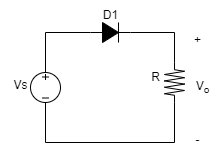
\includegraphics[width=1\linewidth]{Experiment_02/Circuits/Lab2a.png}
                \caption{Half-wave rectifier}
                \label{cir:2a}
            \end{subfigure}
            \begin{subfigure}{0.4\textwidth}
                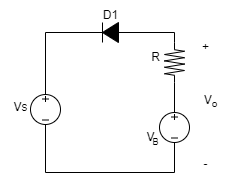
\includegraphics[width=1\linewidth]{Experiment_02/Circuits/Lab2b.png}
                \caption{Clipper circuit}
                \label{cir:2b}
            \end{subfigure}

            \begin{subfigure}{0.4\textwidth}
                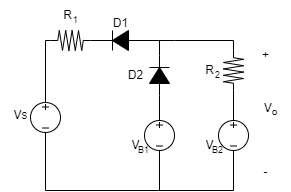
\includegraphics[width=1\linewidth]{Experiment_02/Circuits/Lab2c.png}
                \caption{Clipper circuit IIII}
                \label{cir:2c}
            \end{subfigure}
            \begin{subfigure}{0.4\textwidth}
                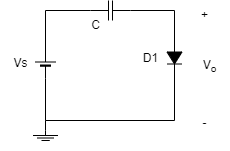
\includegraphics[width=1\linewidth]{Experiment_02/Circuits/Lab2d.png}
                \caption{Clamper circuit}
                \label{cir:2d}
            \end{subfigure}

            \caption{The circuit diagrams}
        \end{figure}

    \subsubsection{Theoretical Analysis}
        \begin{enumerate}[a]
            \item \textbf{Half-wave Rectifier}\par
                From the circuit diagram \ref{cir:2a}. One may easily write the output voltage with respect to the input voltage as follows:
                \begin{equation}
                    \begin{cases}
                        V_o = V_s - V_\gamma & V_s \ge V_\gamma\\
                        V_o = 0 & V_s < V_\gamma\\
                    \end{cases}
                \label{eq:2ret}
                \end{equation}
                where $V_s$ is the input voltage, $V_o$ is the output voltage, and $V_\gamma$ is the diode build in voltage.
            
            \item \textbf{Clipper Circuit}\par
                The clipper circuit is a circuit that clips the input voltage to a certain level. According to \ref{cir:2b} The output voltage can be written as follows:
                \begin{equation}
                    \begin{cases}
                        V_o = V_\gamma + V_s & V_B - V_\gamma \ge V_s\\
                        V_o = V_B & V_s > V_B - V_\gamma\\
                    \end{cases}
                \label{eq:2clip}
                \end{equation}
                where $V_s$ is the input voltage, $V_B$ is a DC power supply, $V_o$ is the output voltage, and $V_\gamma$ is the diode build in voltage.
            
            \item \textbf{Clipper Circuit II}\par
                The clipper circuit shown in figure \ref{cir:2c} is a circuit that clips with two limit. And the output voltage have the following expression:
                \begin{equation}
                    \begin{cases}
                        V_o = V_{B_2} & V_s > V_{B_2} - V_\gamma,~\text{Both diodes off}\\
                        V_o = V_{B_2} - R_2(\frac{V_{B_2}-V_\gamma-V_s}{R_1+R_2}) & V_\gamma \le V_s \le V_{B_2} - V_\gamma,~\text{$D_1$ on only}\\
                        V_o = V_\gamma & V_\gamma > V_s,~\text{Both diodes on}\\
                    \end{cases}
                \label{eq:2clip2}
                \end{equation}
                where $V_s$ is the input voltage, $V_{B1}$ and $V_{B2}$ are DC power supply, $V_o$ is the output voltage, and $V_\gamma$ is the diode build in voltage.
                
            \item \textbf{Clamper Circuit}\par
                Circuit shown in figure \ref{cir:2d} is a clamper circuit. Such circuit will
                The output voltage can be written as follows:
                \begin{equation}
                    \begin{cases}
                        V_o = V_s(sin\omega t-1) & V_s > 0\\
                        V_o = V_s - V_C & V_s < 0\\
                    \end{cases}
                \label{eq:2clam}
                \end{equation}
                where $V_s$ is the input voltage, $V_{B1}$ is a DC power supply, $V_o$ is the output voltage, and $V_\gamma$ is the diode build in voltage.
        \end{enumerate}

\subsection{Experiment record}
    \subsubsection{Half-wave Rectifier}
    \begin{enumerate}[I]
        \item \textbf{Data Recorded}\newline
            The recorded data for the integration operation circuit is shown in the following table \ref{tab:}:
            \begin{table}[h]
                \centering
                \begin{tabular}{l|cccccccc}
                    \hline
                    \toprule
                    Vs   & -3     & -2.8   & -2.6   & -2.4   & -2.2   & -2    & -1.8  & -1.6   \\
                    \midrule
                    Vo   & 0      & 0      & 0      & 0      & 0      & 0     & 0     & 0      \\
                    Theo & 0      & 0      & 0      & 0      & 0      & 0     & 0     & 0      \\
                    \midrule
                    \midrule
                    Vs   & -1.4   & -1.2   & -1     & -0.8   & -0.6   & -0.4  & -0.2  & 0      \\
                    \midrule
                    Vo   & 0      & 0      & 0      & 0      & 0      & 0     & 0     & 0      \\
                    Theo & 0      & 0      & 0      & 0      & 0      & 0     & 0     & 0      \\
                    \midrule
                    \midrule
                    Vs   & 0.2    & 0.4    & 0.6    & 0.8    & 1      & 1.2   & 1.4   & 1.6    \\
                    \midrule
                    Vo   & 0.2m   & 10.48m & 101.3m & 0.2587 & 0.431  & 0.614 & 7993  & 0.9886 \\
                    Theo & 0      & 0      & 0      & 0.2    & 0.4    & 0.6   & 0.8   & 1      \\
                    \midrule
                    \midrule
                    Vs   & 1.8    & 2      & 2.2    & 2.4    & 2.6    & 2.8   & 3     &        \\
                    \midrule
                    Vo   & 1.1758 & 1.3674 & 1.561  & 1.752  & 1.9457 & 2.145 & 2.343 &        \\
                    Theo & 1.2    & 1.4    & 1.6    & 1.8    & 2      & 2.2   & 2.4   &        \\
                    \midrule
                \end{tabular}
                \caption{Recorded Data for half-wave rectifier}
                \label{tab:2ret}
            \end{table}
        And here are the plot of response with respect to the input signal:
        \begin{figure}[H]
            \centering
            \begin{subfigure}{0.45\textwidth}
                \includegraphics[width=1\linewidth]{Experiment_02/Images/2.4_sin_halfWave.jpg}
                \caption{Sin input signal}
                \label{wave:2aSin}
            \end{subfigure}
            \begin{subfigure}{0.45\textwidth}
                \includegraphics[width=1\linewidth]{Experiment_02/Images/2.4_tri_halfWave.jpg}
                \caption{Triangular input signal}
                \label{wave:2aTri}
            \end{subfigure}
            \caption{The output singal of half-wave rectifier}
        \end{figure}

        \item \textbf{Data Analysis}\newline
            The theoretical output voltage of the half-wave rectifier is caculated according to equation \ref{eq:2ret}, and was put into the table tab\ref{tab:2ret} for reference.\par

            According to the table, the measured output voltage is consistent with the theoretical output voltage. This means the half-wave rectifier works as expected.\par

            In the wavefrom plot in fig\ref{wave:2aSin} and fig\ref{wave:2aTri}, we can see half of the input signal is being clipped by the rectifier, and was reduced by the diode build-in voltage.\par
    \end{enumerate}


    \subsubsection{Clipper Circuit}
    \begin{enumerate}[I]
        \item \textbf{Data Recorded}\newline
            The recorded data for the integration operation circuit is shown in the following table \ref{tab:}:
            \begin{table}[h]
                \centering
                \begin{tabular}{l|cccccccc}
                    \hline
                    \midrule
                    Vs   & -3     & -2.8   & -2.6   & -2.4   & -2.2  & -2     & -1.8   & -1.6   \\
                    Vo   & -2.317 & -2.125 & -1.923 & -1.73  & -1.53 & -1.338 & -1.142 & -0.947 \\
                    Theo & -2.4   & -2.2   & -2     & -1.8   & -1.6  & -1.4   & -1.2   & -1     \\
                    \midrule
                    \midrule
                    Vs   & -1.4   & -1.2   & -1     & -0.8   & -0.6  & -0.4   & -0.2   & 0      \\
                    Vo   & -0.754 & -0.564 & -0.364 & -0.177 & 0.015 & 0.208  & 0.388  & 0.568  \\
                    Theo & -0.8   & -0.6   & -0.4   & -0.2   & 0     & 0.2    & 0.4    & 0.6    \\
                    \midrule
                    \midrule
                    Vs   & 0.2    & 0.4    & 0.6    & 0.8    & 1     & 1.2    & 1.4    & 1.6    \\
                    Vo   & 0.744  & 0.899  & 0.989  & 0.999  & 0.999 & 0.999  & 0.999  & 0.999  \\
                    Theo & 0.8    & 1      & 1      & 1      & 1     & 1      & 1      & 1      \\
                    \midrule
                    \midrule
                    Vs   & 1.8    & 2      & 2.2    & 2.4    & 2.6   & 2.8    & 3      &        \\
                    Vo   & 0.999  & 0.999  & 0.999  & 0.999  & 0.999 & 0.999  & 0.999  &        \\
                    Theo & 1      & 1      & 1      & 1      & 1     & 1      & 1      &        \\
                    \midrule
                \end{tabular}
                    \caption{Recorded Data for half-wave rectifier}
                \label{tab:2clip}
            \end{table}
        And here are the plot of response with respect to the input signal:
        \begin{figure}[H]
            \centering
            \begin{subfigure}{0.45\textwidth}
                \includegraphics[width=1\linewidth]{Experiment_02/Images/2.5_sin_clipper1.jpg}
                \caption{Sin input signal}
                \label{wave:2bSin}
            \end{subfigure}
            \begin{subfigure}{0.45\textwidth}
                \includegraphics[width=1\linewidth]{Experiment_02/Images/2.5_tri_clipper1.jpg}
                \caption{Triangular input signal}
                \label{wave:2bTri}
            \end{subfigure}
            \caption{The output singal of Clipper circuit}
        \end{figure}
        
        \item \textbf{Data Analysis}\newline
            The theoretical output voltage of the half-wave rectifier is caculated according to equation \ref{eq:2clip}, and was put into the table tab\ref{tab:2clip} for reference.\par

            According to the table, the measured output voltage is consistent with the theoretical output voltage. This means the clipper circuit works as expected.\par

            In the wavefrom plot in fig\ref{wave:2bSin} and fig\ref{wave:2bTri}, we can see the input signal is clipped by the circuit, and only portion of the input is shown in output.\par
    \end{enumerate}

    \subsubsection{Clipper Circuit II}
    \begin{enumerate}[I]
        \item \textbf{Data Recorded}\newline
            The recorded data for the integration operation circuit is shown in the following table \ref{tab:}:
            \begin{table}[h]
                \centering
                \begin{tabular}{l|ccccccc}
                    \toprule
                    Vs   & 0     & 0.5   & 1     & 1.5   & 2     & 2.5   & 3     \\
                    Vo   & 4.548 & 4.585 & 4.827 & 5.073 & 5.321 & 5.569 & 5.817 \\
                    Theo & 4.449 & 4.449 & 4.449 & 4.449 & 4.449 & 4.449 & 4.449 \\
                    \midrule
                    \midrule
                    Vs   & 3.5   & 4     & 4.5   & 5     & 5.5   & 6     & 6.5   \\
                    Vo   & 6.066 & 6.312 & 6.561 & 6.805 & 7.05  & 7.294 & 7.534 \\
                    Theo & 4.449 & 4.865 & 5.319 & 6.364 & 6.818 & 7.273 & 7.727 \\
                    \midrule
                    \midrule
                    Vs   & 7     & 7.5   & 8     & 8.5   & 9     & 9.5   & 10    \\
                    Vo   & 7.765 & 7.966 & 7.994 & 7.994 & 7.994 & 7.994 & 7.994 \\
                    Theo & 7.137 & 8     & 8     & 8     & 8     & 8     & 8     \\
                    \midrule
                \end{tabular}
                    \caption{Recorded Data for half-wave rectifier}
                \label{tab:2clip2}
            \end{table}
        And here are the plot of response with respect to the input signal:
        \begin{figure}[H]
            \centering
            \begin{subfigure}{0.45\textwidth}
                \includegraphics[width=1\linewidth]{Experiment_02/Images/2.6_sin_clipper2.jpg}
                \caption{Sin input signal}
                \label{wave:2cSin}
            \end{subfigure}
            \begin{subfigure}{0.45\textwidth}
                \includegraphics[width=1\linewidth]{Experiment_02/Images/2.6_tri_clipper2.jpg}
                \caption{Triangular input signal}
                \label{wave:2cTri}
            \end{subfigure}
            \caption{The output singal of Clipper circuit II}
        \end{figure}
        
        \item \textbf{Data Analysis}\newline
            The theoretical output voltage of the half-wave rectifier is caculated according to equation \ref{eq:2clip2}, and was put into the table tab\ref{tab:2clip2} for reference.\par

            According to the table, the measured output voltage is consistent with the theoretical output voltage. This means the clipper circuit works as expected.\par

            In the wavefrom plot in fig\ref{wave:2cSin} and fig\ref{wave:2cTri}, we can see the top and bottom of the input signal is clipped by the circuit, and only portion of the input is shown in output.\par
    \end{enumerate}

    \subsubsection{Clamper Circuit}
    \begin{enumerate}[I]
        \item \textbf{Data Recorded}\newline
            The recorded plot of response with respect to the input signal:
        \begin{figure}[H]
            \centering
            \includegraphics[width=0.5\linewidth]{Experiment_02/Images/2.7_sin_clamper.jpg}
            \caption{The output singal of Clamper circuit}
            \label{wave:2dSin}
        \end{figure}
        
        \item \textbf{Data Analysis}\newline
            In the wavefrom plot in fig\ref{wave:2dSin}, we can see the output signal is shit downward in the y axis. This is beacuse the capacitor will be charge when the input signal is positive, and slowly discharge when the input signal is negetive.\par
    \end{enumerate}
    
\subsection{Experiment Conclusion}
    \subsubsection{Conclusion}
    In this experiment, we constructed three types of diode circuit, and tested their behaviour using the DMM and Oscilloscope. Finally, we conclude our calculation is correct.
\section{Diode Rectifier Circuits}

\subsection{Experiment Design}
    \subsubsection{Background}
        In the previous chapter, we constructed a half wave rectifier. However, the half wave rectifier has a low efficiency and produces a large ripple voltage. In this chapter, we will construct a full wave rectifier to overcome these disadvantages. The full wave rectifier can be constructed in vairious way, in this experiment, we will construct two types of full wave rectifier: the full wave rectifier with center-tapped transformer and the full wave bridge rectifier.

    \subsubsection{Propose}
    \begin{itemize}
        \item To verify a full-wave rectifier with center-tapped transformer
        \item To verify a full-wave bridge rectifier
    \end{itemize}

\subsection{Experiment Design}
    \subsubsection{Materials}
        In this experiment, we will use the following components:
        \begin{itemize}
            \item 1N4148 Diode
            \item Resistors
            \item Transformers
            \item Breadboard
            \item DC power supply
            \item Digital Multi-Meter
            \item Function Generator
            \item Oscilloscope
        \end{itemize}

    \subsubsection{Circuit Diagram}
        The following circuit diagrams 
        \begin{figure}[H]
            \centering
            \begin{subfigure}{0.6\textwidth}
                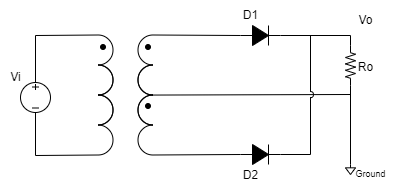
\includegraphics[width=1\linewidth]{Experiment_03/Circuits/Lab3a.png}
                \caption{Center Tapped Full-wave diode rectifier}
                \label{cir:3a}
            \end{subfigure}

            \begin{subfigure}{0.6\textwidth}
                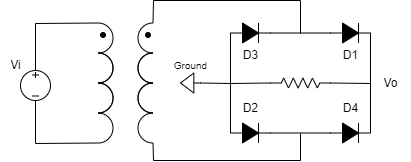
\includegraphics[width=1\linewidth]{Experiment_03/Circuits/Lab3b.png}
                \caption{Bridge Full-wave bridge diode rectifier}
                \label{cir:3b}
            \end{subfigure}
            \caption{Circuit of Diode Rectifier}
        \end{figure}

    \subsubsection{Theoretical Analysis}
        \begin{enumerate}[a]
            \item \textbf{Center Tapped Diode Rectifier}\par
                Center-Tapped Full-wave Rectifier uses two diodes. By using a transformer with two terminal, It split the AC output into two equal halves. And the two diodes conduct during each half of the AC cycle, producing a full-wave rectified output.
            \item \textbf{Bridge Full-wave Rectifier}\par
                Bridge Full-wave Rectifier uses four diodes. During both halves of the AC input cycle, two of the four diodes conduct, ensuring that current flows in the same direction through the load, providing a full-wave rectified output.
        \end{enumerate}

\subsection{Experiment record}
    \subsubsection{Center Tapped Full-wave Rectifier}
    \begin{enumerate}[I]
        \item \textbf{Data Recorded}\newline
            The recorded data for the center-tapped full wave rectifier circuit is shown in the following picture:
            \begin{figure}[h]
                \centering
                \begin{subfigure}[h]{0.4\textwidth}
                    \centering
                    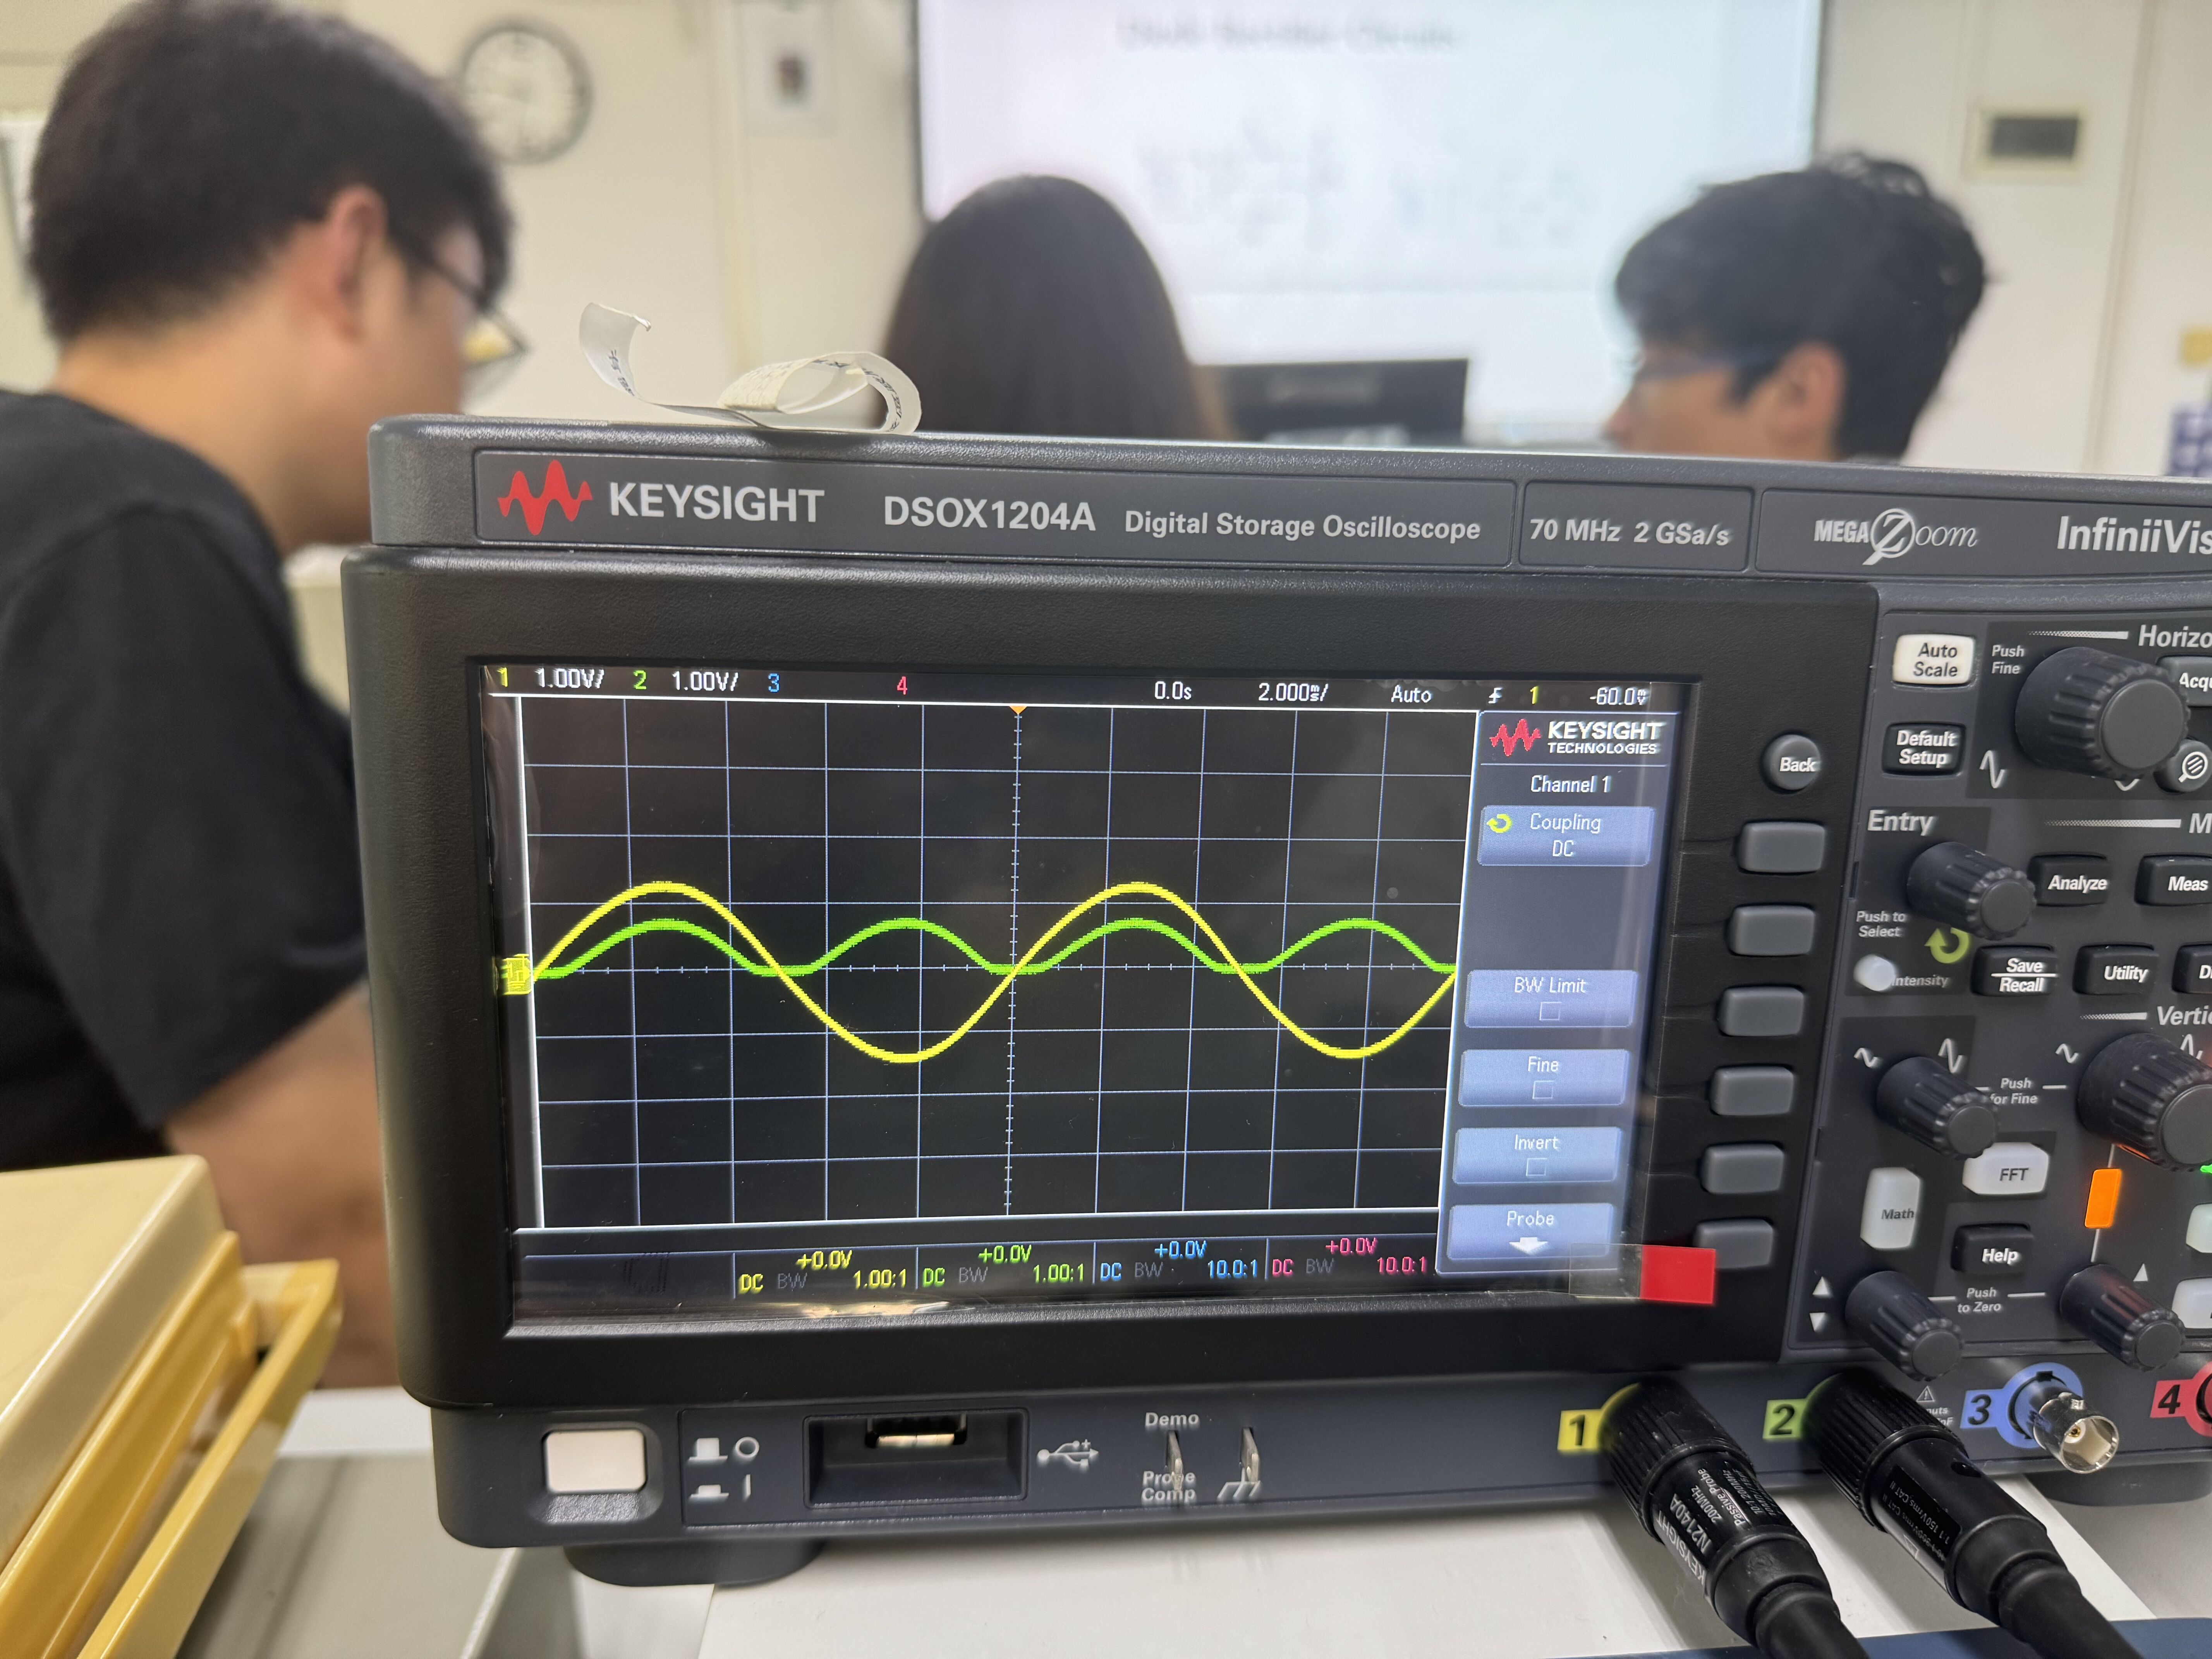
\includegraphics[width=1\textwidth]{Experiment_03/Images/3.4_outPutVoltage.jpg}
                    \caption{Output Voltage}
                    \label{wave:3.4OV}
                \end{subfigure}
                \begin{subfigure}[h]{0.4\textwidth}
                    \centering
                    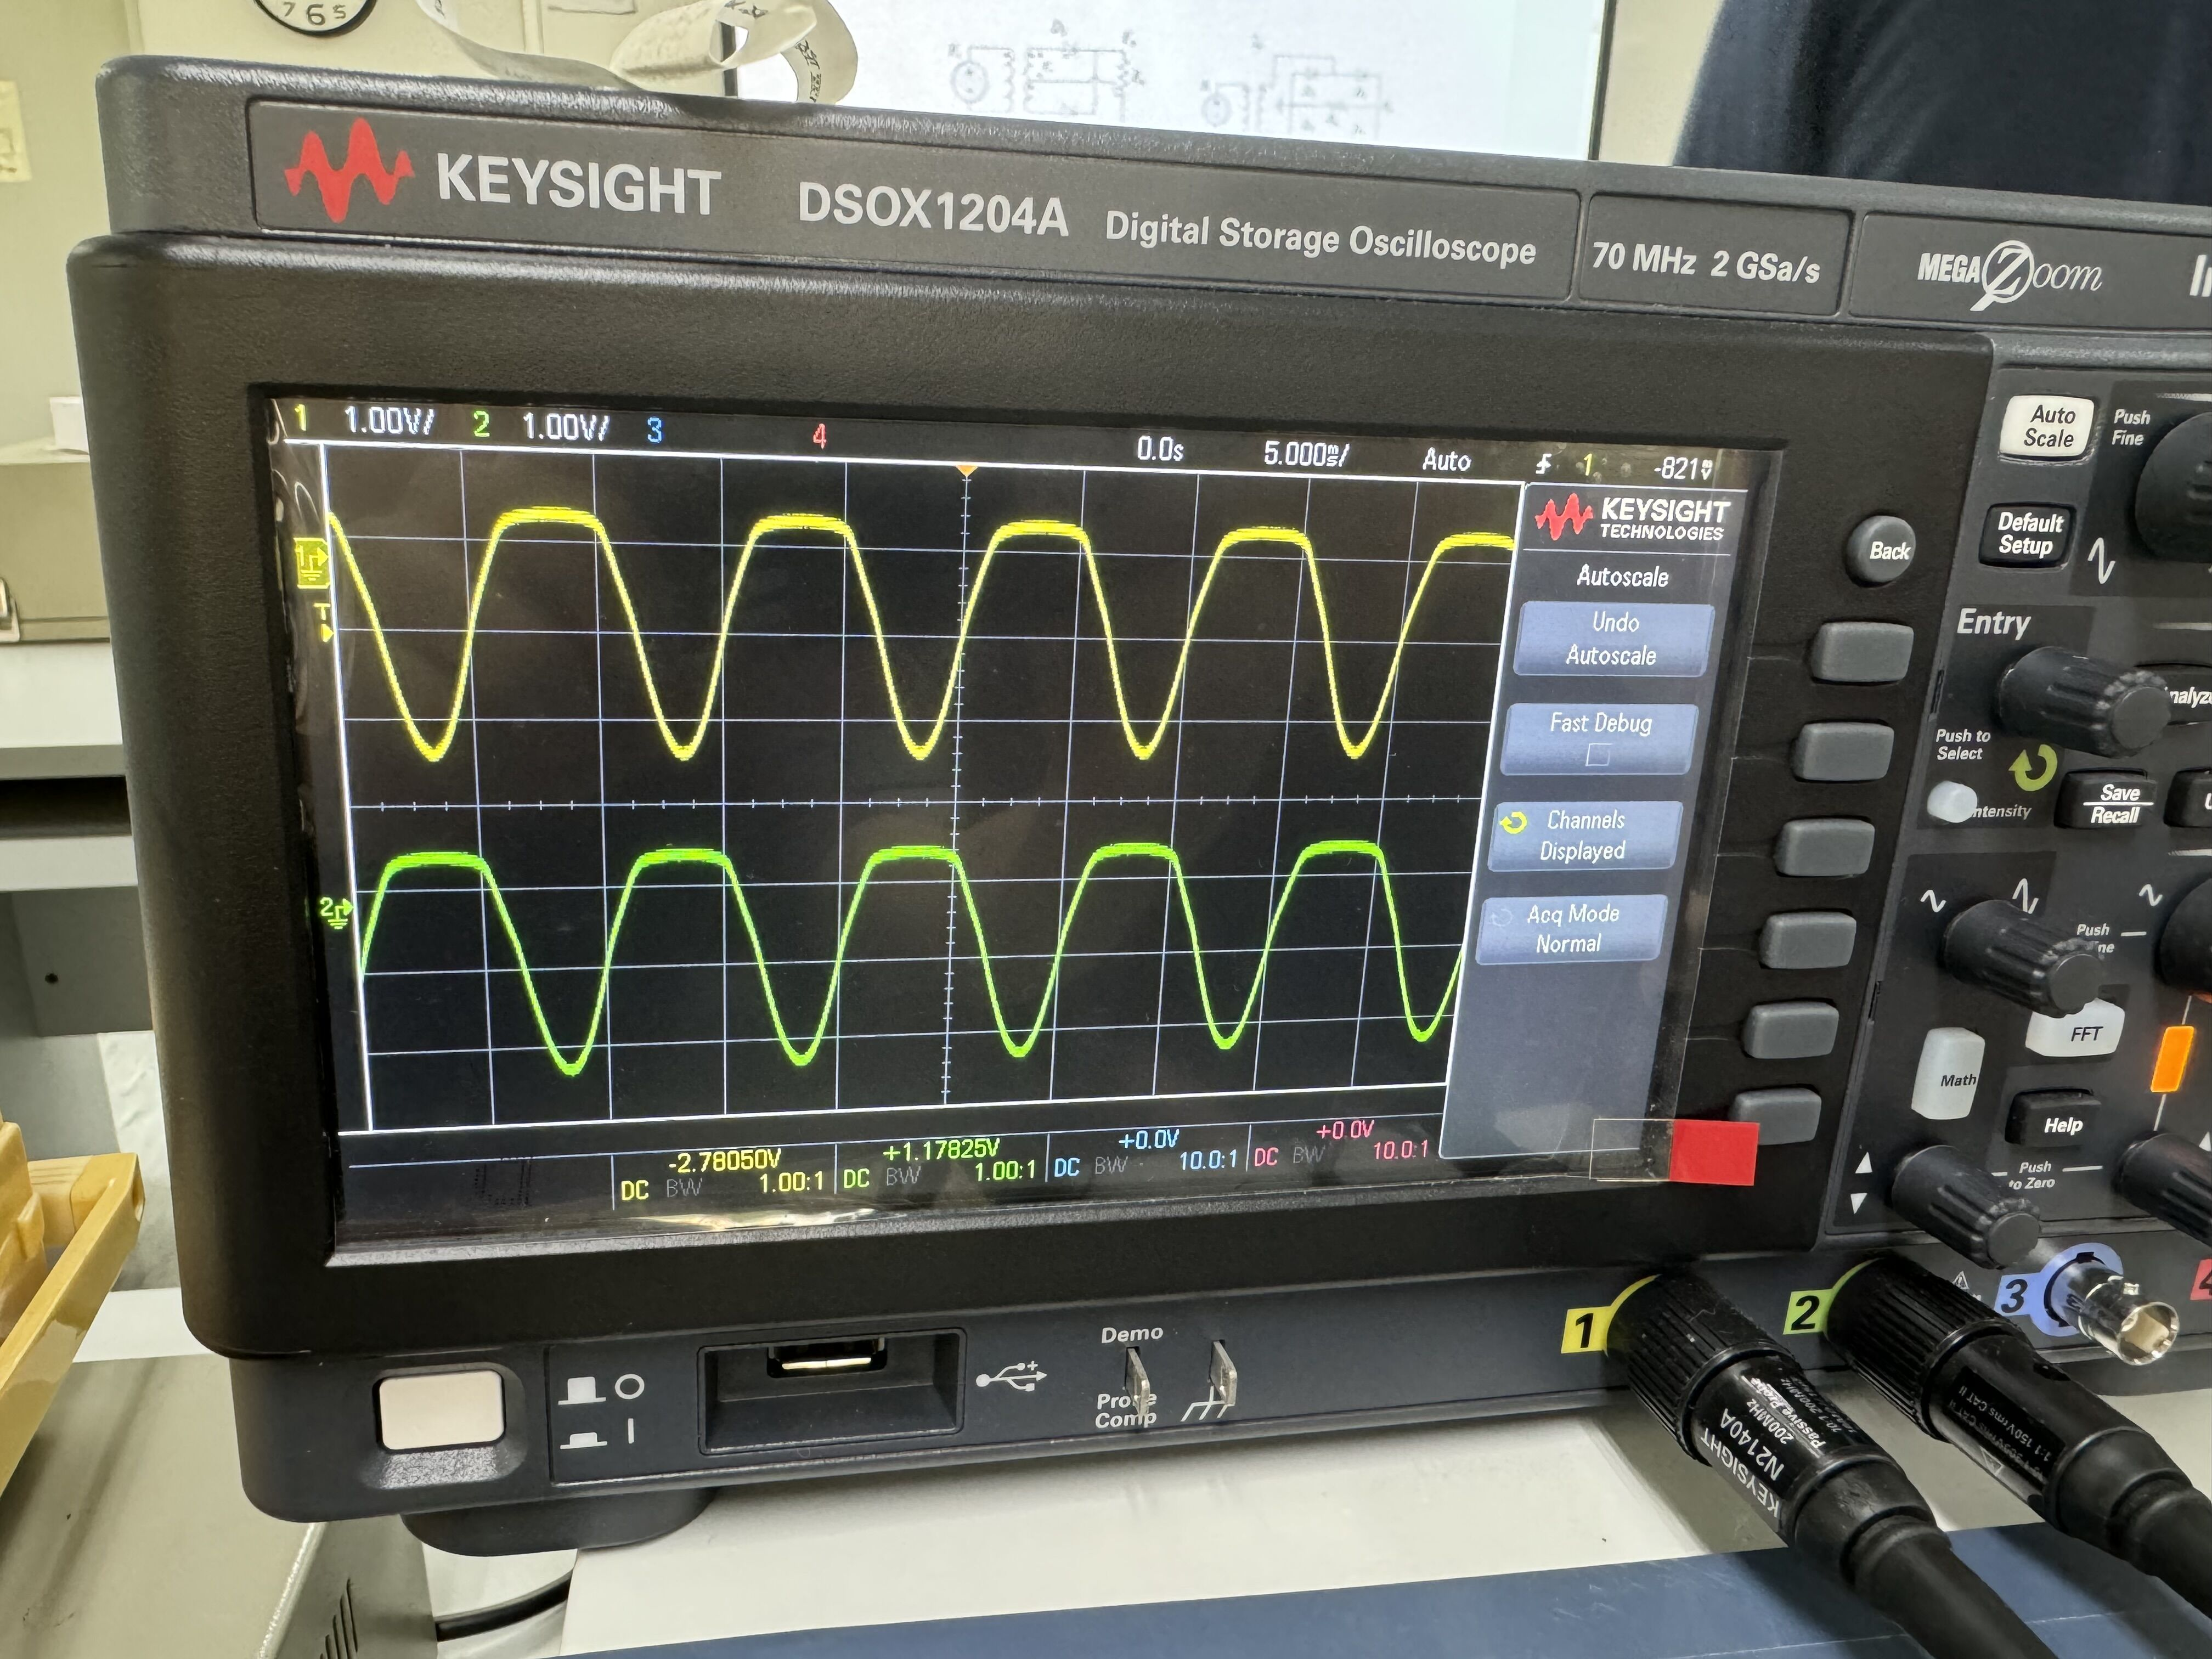
\includegraphics[width=1\textwidth]{Experiment_03/Images/3.4_diodeVoltage.jpg}
                    \caption{Diode Voltage}
                    \label{wave:3.4DV}
                \end{subfigure}
            \end{figure}
        \item \textbf{Data Analysis}\newline
            From Fig.\ref{wave:3.4OV}, we can see the negetive signal from input is flipped, and the output signal have an amplitude about half of the input signal. This is because the Center-Tapped transformer split the input signal into two protion with half of original energy.\par
            
            And Fig.\ref{wave:3.4DV} shows two diodes are working alternatively.
    \end{enumerate}

    \subsubsection{Bridge Full-wave Rectifier}
    \begin{enumerate}[I]
        \item \textbf{Data Recorded}\newline
            The recorded data for the bridge full wave rectifier circuit is shown in the following picture:
            \begin{figure}[h]
                \centering
                \begin{subfigure}[h]{0.4\textwidth}
                    \centering
                    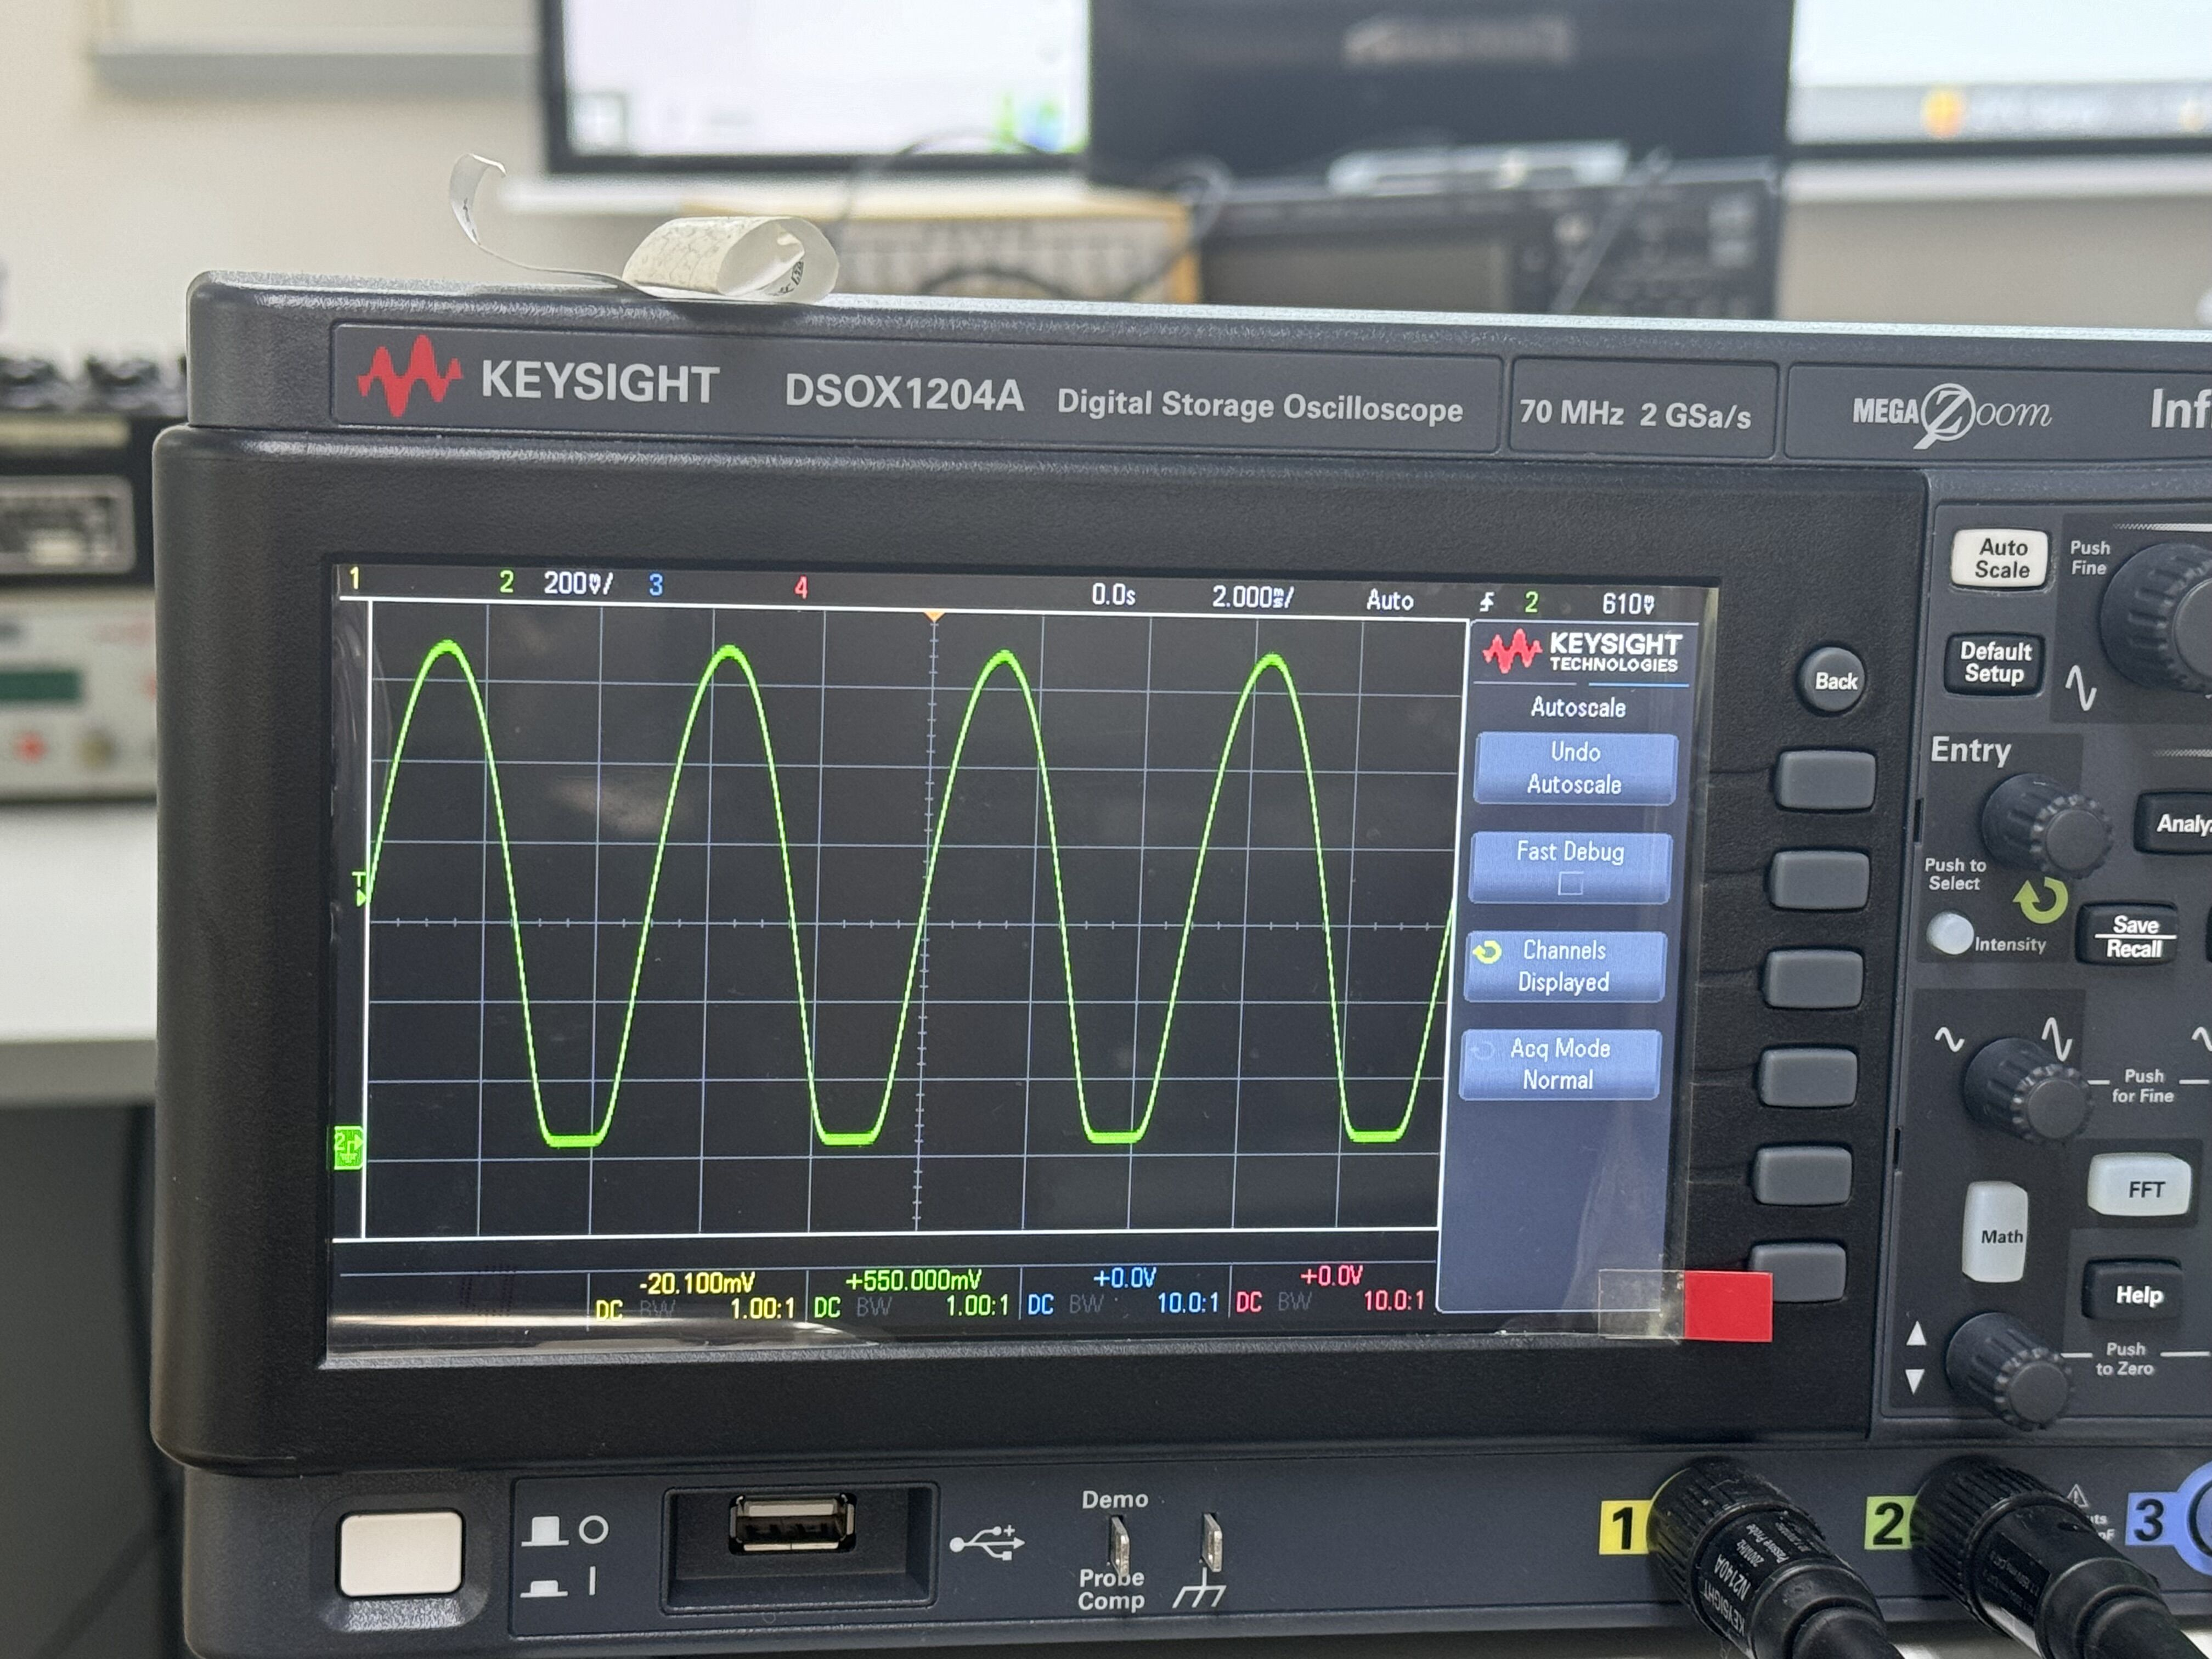
\includegraphics[width=1\textwidth]{Experiment_03/Images/3.5_outPutVoltage.jpg}
                    \caption{Output Voltage}
                    \label{wave:3.5OV}
                \end{subfigure}
                \begin{subfigure}[h]{0.4\textwidth}
                    \centering
                    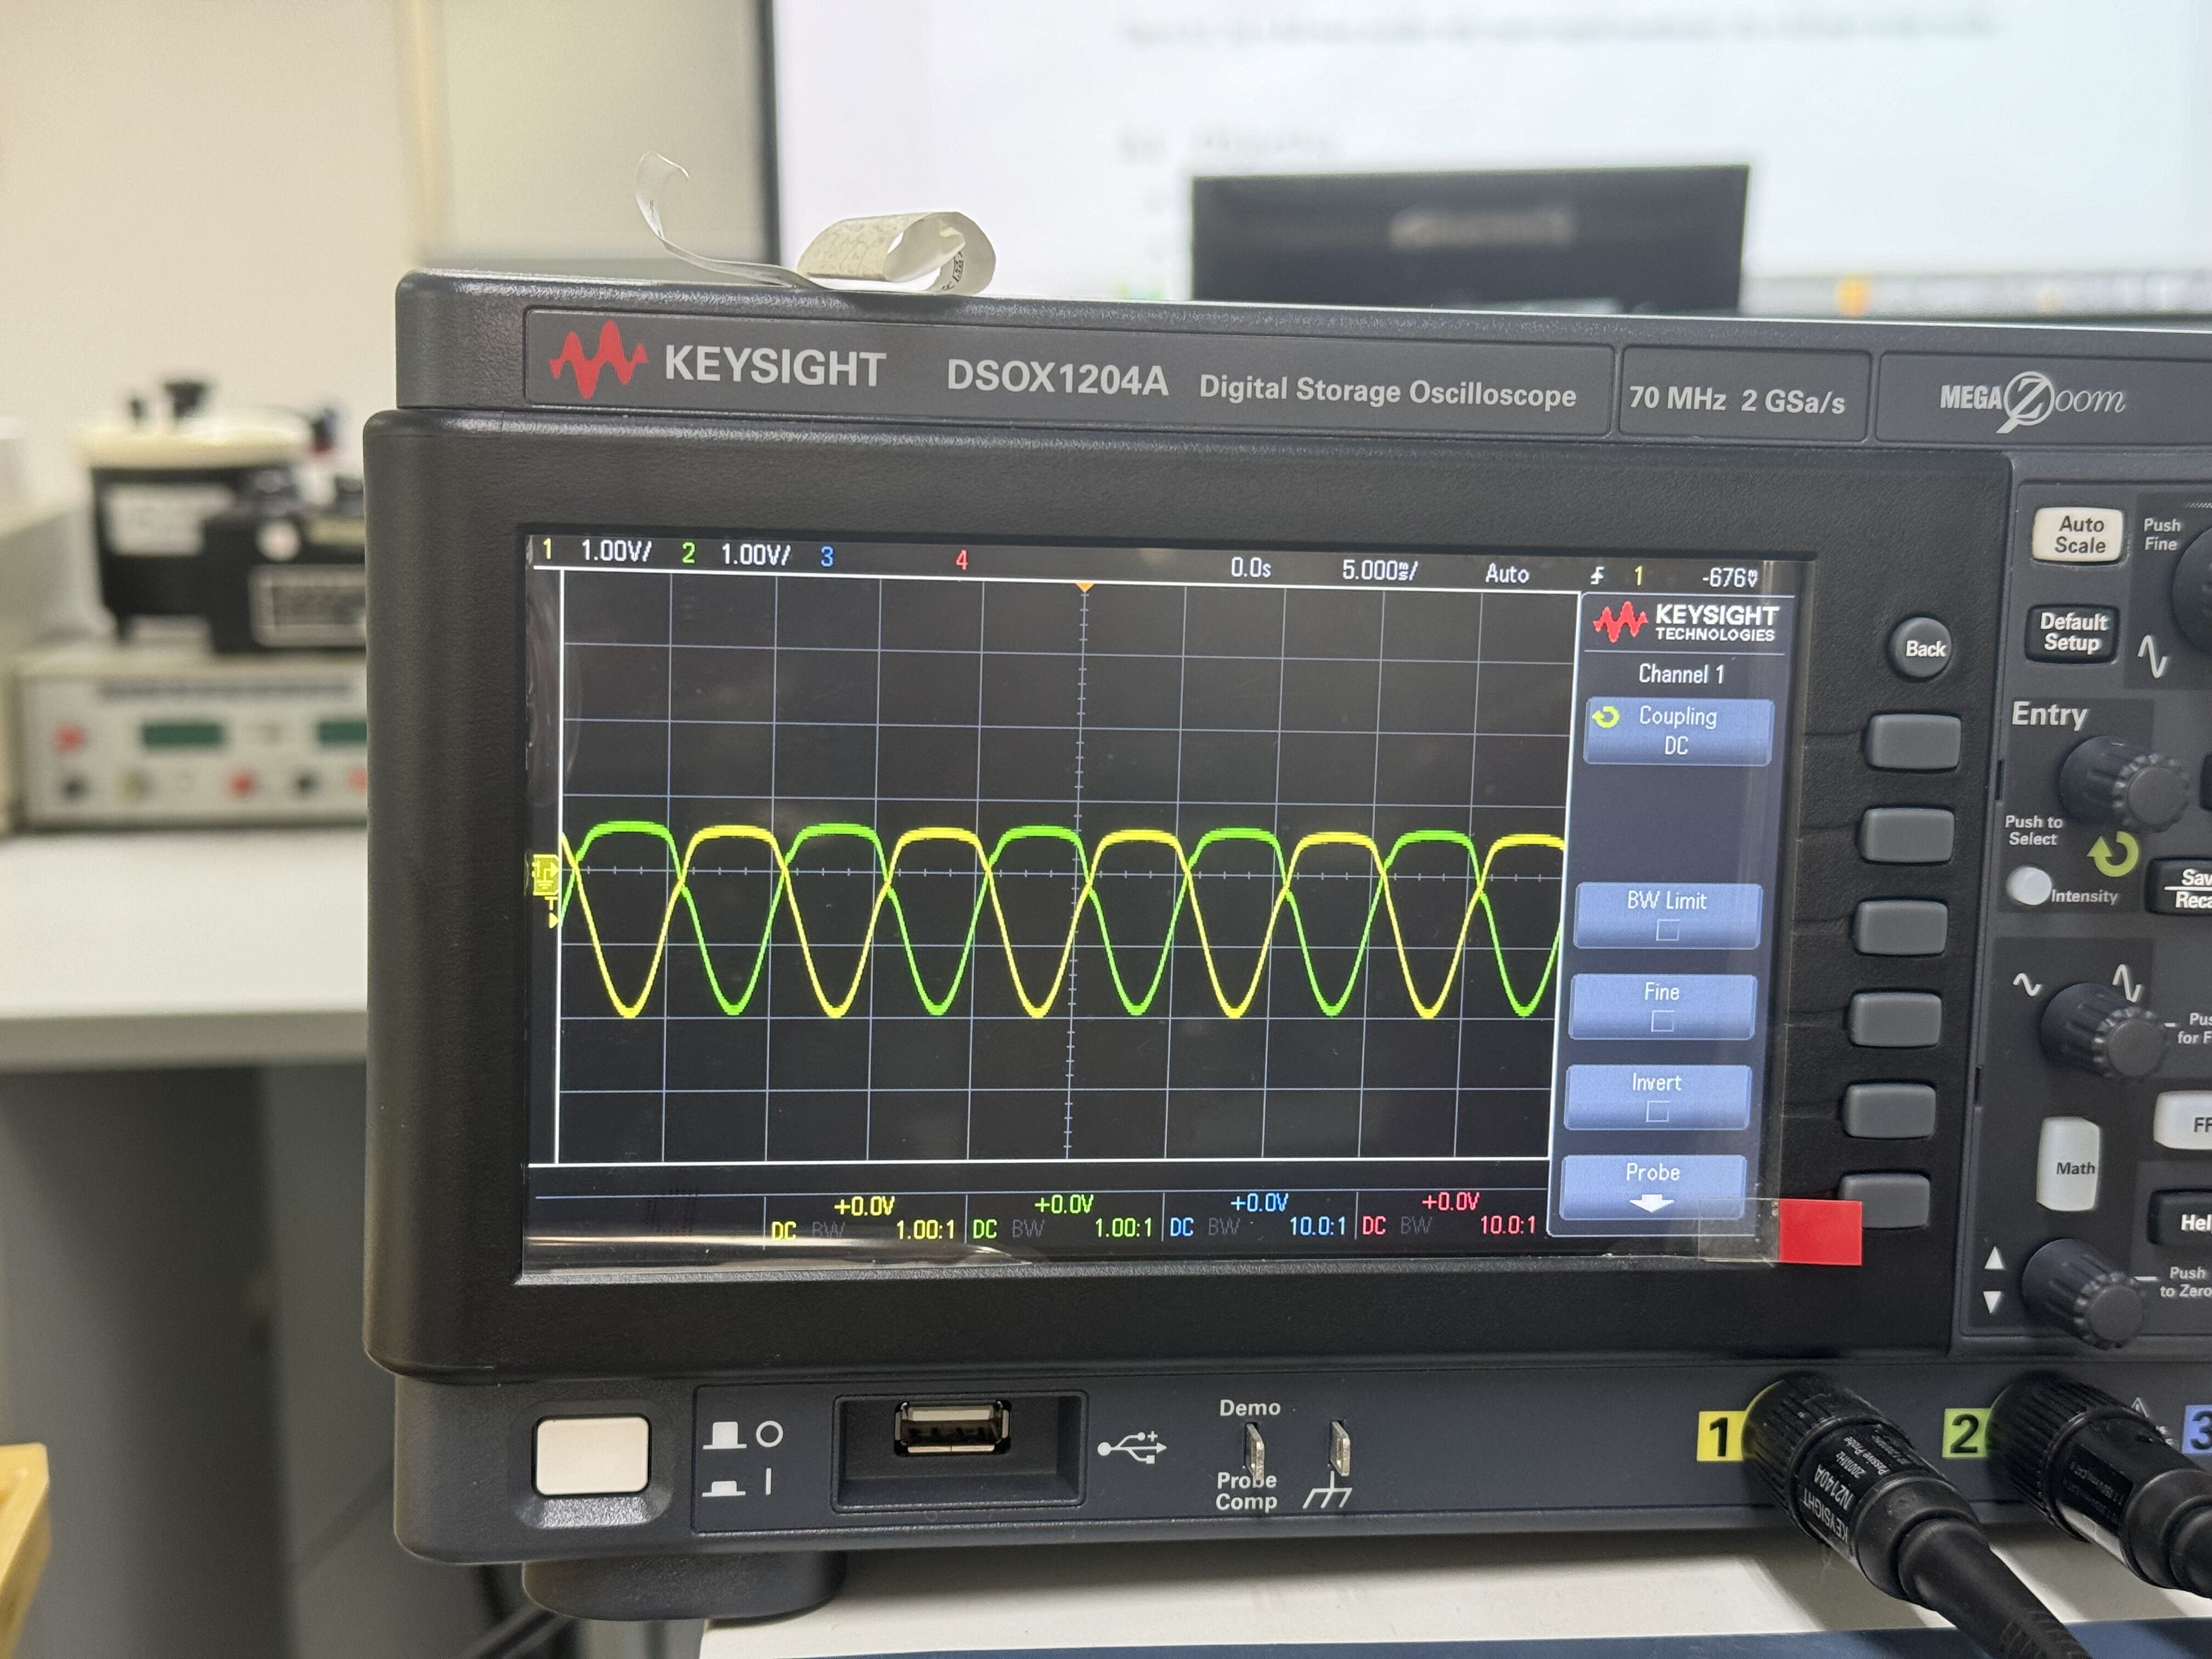
\includegraphics[width=1\textwidth]{Experiment_03/Images/3.5_diodeVoltage.jpg}
                    \caption{Diode Voltage}
                    \label{wave:3.5DV}
                \end{subfigure}
            \end{figure}
        \item \textbf{Data Analysis}\newline
            From Fig.\ref{wave:3.5OV}, we can see the output signal have same amplitude as the original signal. In addition,the output have a smaller ripple voltage than the Center-Tapped Full-wave Rectifier. This is because the Bridge Full-wave Rectifier use four diodes to conduct the current, which provide a more stable output signal.\par
            
            And Fig.\ref{wave:3.5DV} shows the two paires of diodes are working alternatively.
    \end{enumerate}
    
\subsection{Experiment Conclusion}
    \subsubsection{Discussion}
        In this experiment, we notice the Center-Tapped Full-wave Rectifier and Bridge Full-wave Rectifier have different advantage. The Center-Tapped Full-wave Rectifier is chaper and easier to construct, but it has a lower efficiency and produce a larger ripple voltage. On the other hand, the Bridge Full-wave Rectifier is more expensive and complex, but it has a higher efficiency and produce a smaller ripple voltage.
    \subsubsection{Conclusion}
\section{Common-Emitter Current Gain}

\subsection{Experiment Design}
    \subsubsection{Background}
        In this experiment, we are going to learn common-emitter BJT circuits. A DC source, resistors, and an npn BJT will be used to construct the circuits, the digital multi-meter is used to measure $V_{BE}$ and $V_{CE}$.\par

    \subsubsection{Propose}
    \begin{itemize}
        \item Find the Common-Emitter Current Gain of a npn BJT
    \end{itemize}

\subsection{Experiment Design}
    \subsubsection{Materials}
        In this experiment, we will use the following components:
        \begin{itemize}
            \item 2N3904 BJT
            \item Resistors
            \item Breadboard
            \item DC power supply
            \item Digital Multi-Meter
        \end{itemize}

    \subsubsection{Circuit Diagram}
        The following circuit diagrams 
        \begin{figure}[H]
            \centering
                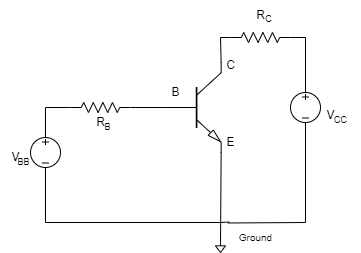
\includegraphics[width=0.6\linewidth]{Experiment_04/Circuits/Lab4.png}
                \caption{Common-Emitter Connection}
                \label{cir:4}
        \end{figure}

    \subsubsection{Theoretical Analysis}
        Common Emitter BJT means the emitter is connect to the common ground with the input source. The common-emitter BJT is usually used for amplification due to its high voltage and current gain.\par

        And according to the circuit shown in Fig.\ref{cir:4}, we can write the following equations:
        \begin{align}
            & V_{BB} - i_BR_B - V_{BE} = 0
            \label{eq:4.1}\\ 
            & V_{CC} - i_CR_C - V_{CE} = 0
            \label{eq:4.2}\\
            & i_C = \frac{V_{CC} - V_{CE}}{R_C}
            \label{eq:4.3}\\
            & i_C = \beta i_B
            \label{eq:4.4}
        \end{align}
        \par

        With this information, we can calculate the current gain by measure the $V_{BE}$ and $V_{CE}$. Then, we can plot the relation between $I_C$ and $V_{CE}$ to find the current gain.
        And subtitude \ref{eq:4.1} into \ref{eq:4.4}, we have the expression for current $I_C$ in normal operation:

        \begin{equation}
            I_C \approx \frac{V_{CC} - V_{CE}}{R_C + \frac{R_B}{\beta}}
            \label{eq:4.5}
        \end{equation}



\subsection{Experiment record}
    \subsubsection{Data Measurement}
    To avoid error in the resistor, we first measure the resistance of the resistors. The measured resistance is shown in the following table:
    \begin{table}[H]
        \centering
        \begin{tabular}{l|c}
            \hline
            $R_C$ & 0.9899k $\Omega$\\
            $R_B$ & 55.33k$\Omega$\\
            \hline
        \end{tabular}
        \caption{Measured Resistance}
        \label{tab:4.1}
    \end{table}\par

    Next, we meausre the $V_{BE}$ and $V_{CE}$ of the BJT, and calculate the corresponding $I_C$ for different $V_{BB}$. The measured data is shown in the following table:
    \begin{table}[H]
    \centering
        \begin{tabular}{ccccccccc}
            \midrule
        \multicolumn{9}{c}{$V_{BB}=1.0V$}                                                                                                                                                                                                                     \\
        \midrule
        \multicolumn{1}{l|}{Vcc}     & \multicolumn{1}{c}{0.1}    & \multicolumn{1}{c}{0.2}    & \multicolumn{1}{c}{0.4}    & \multicolumn{1}{c}{0.6}    & \multicolumn{1}{c}{0.8}    & \multicolumn{1}{c}{1}      & \multicolumn{1}{c}{2}     & 3      \\
        \multicolumn{1}{l|}{Vbe}     & \multicolumn{1}{c}{0.5698} & \multicolumn{1}{c}{0.587}  & \multicolumn{1}{c}{0.606}  & \multicolumn{1}{c}{0.617}  & \multicolumn{1}{c}{0.625}  & \multicolumn{1}{c}{0.631}  & \multicolumn{1}{c}{0.65}  & 0.652  \\
        \multicolumn{1}{l|}{Vce}     & \multicolumn{1}{c}{0.04}   & \multicolumn{1}{c}{0.06}   & \multicolumn{1}{c}{0.084}  & \multicolumn{1}{c}{0.1}    & \multicolumn{1}{c}{0.112}  & \multicolumn{1}{c}{0.123}  & \multicolumn{1}{c}{0.189} & 0.929  \\
        \multicolumn{1}{l|}{Ib}      & \multicolumn{1}{c}{7.8u}   & \multicolumn{1}{c}{7.5u}   & \multicolumn{1}{c}{7.1u}   & \multicolumn{1}{c}{6.9u}   & \multicolumn{1}{c}{6.8u}   & \multicolumn{1}{c}{6.7u}   & \multicolumn{1}{c}{6.3u}  & 6.3u   \\
        \multicolumn{1}{l|}{Ic}      & \multicolumn{1}{c}{0.061}  & \multicolumn{1}{c}{0.141}  & \multicolumn{1}{c}{0.319}  & \multicolumn{1}{c}{0.505}  & \multicolumn{1}{c}{0.695}  & \multicolumn{1}{c}{0.886}  & \multicolumn{1}{c}{1.829} & 2.092  \\
        \multicolumn{1}{l|}{$\beta$} & \multicolumn{1}{c}{7.8k}   & \multicolumn{1}{c}{19k}    & \multicolumn{1}{c}{45k}    & \multicolumn{1}{c}{73k}    & \multicolumn{1}{c}{100k}   & \multicolumn{1}{c}{130k}   & \multicolumn{1}{c}{290k}  & 330k   \\
        \midrule
        \midrule
        \multicolumn{1}{l|}{Vcc}     & \multicolumn{1}{c}{4}      & \multicolumn{1}{c}{5}      & \multicolumn{1}{c}{6}      & \multicolumn{1}{c}{7}      & \multicolumn{1}{c}{8}      & \multicolumn{1}{c}{9}      & \multicolumn{1}{c}{10}    & AVG    \\
        \multicolumn{1}{l|}{Vbe}     & \multicolumn{1}{c}{0.651}  & \multicolumn{1}{c}{0.6499} & \multicolumn{1}{c}{0.6485} & \multicolumn{1}{c}{0.6474} & \multicolumn{1}{c}{0.6462} & \multicolumn{1}{c}{0.6452} & \multicolumn{1}{c}{0.645} & 0.6314 \\
        \multicolumn{1}{l|}{Vce}     & \multicolumn{1}{c}{1.91}   & \multicolumn{1}{c}{2.89}   & \multicolumn{1}{c}{3.86}   & \multicolumn{1}{c}{4.84}   & \multicolumn{1}{c}{5.83}   & \multicolumn{1}{c}{6.82}   & \multicolumn{1}{c}{7.8}   &        \\
        \multicolumn{1}{l|}{Ib}      & \multicolumn{1}{c}{6.3u}   & \multicolumn{1}{c}{6.3u}   & \multicolumn{1}{c}{6.4u}   & \multicolumn{1}{c}{6.4u}   & \multicolumn{1}{c}{6.4u}   & \multicolumn{1}{c}{6.4u}   & \multicolumn{1}{c}{6.4u}  & 6.7u   \\
        \multicolumn{1}{l|}{Ic}      & \multicolumn{1}{c}{2.111}  & \multicolumn{1}{c}{2.131}  & \multicolumn{1}{c}{2.162}  & \multicolumn{1}{c}{2.182}  & \multicolumn{1}{c}{2.192}  & \multicolumn{1}{c}{2.202}  & \multicolumn{1}{c}{2.222} &        \\
        \multicolumn{1}{l|}{$\beta$} & \multicolumn{1}{c}{330k}   & \multicolumn{1}{c}{340k}   & \multicolumn{1}{c}{340k}   & \multicolumn{1}{c}{340k}   & \multicolumn{1}{c}{340k}   & \multicolumn{1}{c}{340k}   & \multicolumn{1}{c}{350k}  &        \\
        \midrule
        \end{tabular}
        \caption{Measured Data for $V_{BB}=1.0V$}
        \end{table}


        \begin{table}[H]
            \centering
            \begin{tabular}{ccccccccc}
                \midrule
            \multicolumn{9}{c}{$V_{BB}=1.3V$}\\
            \midrule
            \multicolumn{1}{l|}{Vcc}     & \multicolumn{1}{c}{0.1}      & \multicolumn{1}{c}{0.2}      & \multicolumn{1}{c}{0.4}      & \multicolumn{1}{c}{0.6}      & \multicolumn{1}{c}{0.8}      & \multicolumn{1}{c}{1}        & \multicolumn{1}{c}{2}        & 3        \\
            \multicolumn{1}{l|}{Vbe}     & \multicolumn{1}{c}{0.576}    & \multicolumn{1}{c}{0.591}    & \multicolumn{1}{c}{0.609}    & \multicolumn{1}{c}{0.619}    & \multicolumn{1}{c}{0.627}    & \multicolumn{1}{c}{0.634}    & \multicolumn{1}{c}{0.653}    & 0.664    \\
            \multicolumn{1}{l|}{Vce}     & \multicolumn{1}{c}{0.034}    & \multicolumn{1}{c}{0.05}     & \multicolumn{1}{c}{0.069}    & \multicolumn{1}{c}{0.082}    & \multicolumn{1}{c}{0.092}    & \multicolumn{1}{c}{0.101}    & \multicolumn{1}{c}{0.134}    & 0.169    \\
            \multicolumn{1}{l|}{Ib}      & \multicolumn{1}{c}{13.1u}    & \multicolumn{1}{c}{12.8u}    & \multicolumn{1}{c}{12.5u}    & \multicolumn{1}{c}{12.3u}    & \multicolumn{1}{c}{12.2u}    & \multicolumn{1}{c}{12u}      & \multicolumn{1}{c}{11.7u}    & 11.5u    \\
            \multicolumn{1}{l|}{Ic}      & \multicolumn{1}{c}{0.067}    & \multicolumn{1}{c}{0.152}    & \multicolumn{1}{c}{0.334}    & \multicolumn{1}{c}{0.523}    & \multicolumn{1}{c}{0.715}    & \multicolumn{1}{c}{0.908}    & \multicolumn{1}{c}{1.885}    & 2.860    \\
            \multicolumn{1}{l|}{$\beta$} & \multicolumn{1}{c}{5094.843} & \multicolumn{1}{c}{11824.17} & \multicolumn{1}{c}{26771.67} & \multicolumn{1}{c}{42511.67} & \multicolumn{1}{c}{58795.44} & \multicolumn{1}{c}{75441.61} & \multicolumn{1}{c}{161188}   & 248775.9 \\
            \midrule
            \midrule
            \multicolumn{1}{l|}{Vcc}     & \multicolumn{1}{c}{4}        & \multicolumn{1}{c}{5}        & \multicolumn{1}{c}{6}        & \multicolumn{1}{c}{7}        & \multicolumn{1}{c}{8}        & \multicolumn{1}{c}{9}        & \multicolumn{1}{c}{10}       & AVG      \\
            \multicolumn{1}{l|}{Vbe}     & \multicolumn{1}{c}{0.669}    & \multicolumn{1}{c}{0.668}    & \multicolumn{1}{c}{0.667}    & \multicolumn{1}{c}{0.665}    & \multicolumn{1}{c}{0.664}    & \multicolumn{1}{c}{0.661}    & \multicolumn{1}{c}{0.658}    & 0.641667 \\
            \multicolumn{1}{l|}{Vce}     & \multicolumn{1}{c}{0.325}    & \multicolumn{1}{c}{1.23}     & \multicolumn{1}{c}{2.17}     & \multicolumn{1}{c}{3.13}     & \multicolumn{1}{c}{4.09}     & \multicolumn{1}{c}{5.06}     & \multicolumn{1}{c}{6.01}     &          \\
            \multicolumn{1}{l|}{Ib}      & \multicolumn{1}{c}{11.4u}    & \multicolumn{1}{c}{11.4u}    & \multicolumn{1}{c}{11.4u}    & \multicolumn{1}{c}{11.5u}    & \multicolumn{1}{c}{11.5u}    & \multicolumn{1}{c}{11.5u}    & \multicolumn{1}{c}{11.6u}    & 11.9u    \\
            \multicolumn{1}{l|}{Ic}      & \multicolumn{1}{c}{3.712}    & \multicolumn{1}{c}{3.808}    & \multicolumn{1}{c}{3.869}    & \multicolumn{1}{c}{3.909}    & \multicolumn{1}{c}{3.949}    & \multicolumn{1}{c}{3.980}    & \multicolumn{1}{c}{4.030}    &          \\
            \multicolumn{1}{l|}{$\beta$} & \multicolumn{1}{c}{325501.8} & \multicolumn{1}{c}{333387.8} & \multicolumn{1}{c}{338158.7} & \multicolumn{1}{c}{340614.2} & \multicolumn{1}{c}{343593.6} & \multicolumn{1}{c}{344604.4} & \multicolumn{1}{c}{347346.8} &          \\
        \hline    
        \end{tabular}
            \caption{Measured Data for $V_{BB}=1.3V$}
            \end{table}

            \begin{table}[H]
                \centering
                \begin{tabular}{ccccccccc}
                \hline
                \multicolumn{9}{c}{$V_{BB}=1.7V$}                                                                                                                                                                                                                                      \\ \hline
                \multicolumn{1}{l|}{Vcc}     & \multicolumn{1}{c}{0.1}      & \multicolumn{1}{c}{0.2}      & \multicolumn{1}{c}{0.4}      & \multicolumn{1}{c}{0.6}      & \multicolumn{1}{c}{0.8}      & \multicolumn{1}{c}{1}        & \multicolumn{1}{c}{2}        & 3        \\ 
                \multicolumn{1}{l|}{Vbe}     & \multicolumn{1}{c}{0.584}    & \multicolumn{1}{c}{0.596}    & \multicolumn{1}{c}{0.611}    & \multicolumn{1}{c}{0.621}    & \multicolumn{1}{c}{0.628}    & \multicolumn{1}{c}{0.634}    & \multicolumn{1}{c}{0.653}    & 0.664    \\ 
                \multicolumn{1}{l|}{Vce}     & \multicolumn{1}{c}{0.027}    & \multicolumn{1}{c}{0.04}     & \multicolumn{1}{c}{0.0573}   & \multicolumn{1}{c}{0.06}     & \multicolumn{1}{c}{0.077}    & \multicolumn{1}{c}{0.085}    & \multicolumn{1}{c}{0.112}    & 0.133    \\ 
                \multicolumn{1}{l|}{Ib}      & \multicolumn{1}{c}{20.2u}    & \multicolumn{1}{c}{20u}      & \multicolumn{1}{c}{19.7u}    & \multicolumn{1}{c}{19.5u}    & \multicolumn{1}{c}{19.4u}    & \multicolumn{1}{c}{19.3u}    & \multicolumn{1}{c}{18.9u}    & 18.7u    \\ 
                \multicolumn{1}{l|}{Ic}      & \multicolumn{1}{c}{0.074}    & \multicolumn{1}{c}{0.162}    & \multicolumn{1}{c}{0.346}    & \multicolumn{1}{c}{0.545}    & \multicolumn{1}{c}{0.730}    & \multicolumn{1}{c}{0.924}    & \multicolumn{1}{c}{1.907}    & 2.896    \\ 
                \multicolumn{1}{l|}{$\beta$} & \multicolumn{1}{c}{3655.814} & \multicolumn{1}{c}{8099.839} & \multicolumn{1}{c}{17587.81} & \multicolumn{1}{c}{27970.34} & \multicolumn{1}{c}{37693.72} & \multicolumn{1}{c}{47972.17} & \multicolumn{1}{c}{100781.5} & 154665.5 \\ 
                \hline
                \hline
                \multicolumn{1}{l|}{Vcc}     & \multicolumn{1}{c}{4}        & \multicolumn{1}{c}{5}        & \multicolumn{1}{c}{6}        & \multicolumn{1}{c}{7}        & \multicolumn{1}{c}{8}        & \multicolumn{1}{c}{9}        & \multicolumn{1}{c}{10}       & AVG      \\ 
                \multicolumn{1}{l|}{Vbe}     & \multicolumn{1}{c}{0.672}    & \multicolumn{1}{c}{0.678}    & \multicolumn{1}{c}{0.682}    & \multicolumn{1}{c}{0.68}     & \multicolumn{1}{c}{0.678}    & \multicolumn{1}{c}{0.676}    & \multicolumn{1}{c}{0.673}    & 0.648667 \\ 
                \multicolumn{1}{l|}{Vce}     & \multicolumn{1}{c}{0.156}    & \multicolumn{1}{c}{0.188}    & \multicolumn{1}{c}{0.303}    & \multicolumn{1}{c}{1.044}    & \multicolumn{1}{c}{1.95}     & \multicolumn{1}{c}{2.87}     & \multicolumn{1}{c}{3.76}     &          \\ 
                \multicolumn{1}{l|}{Ib}      & \multicolumn{1}{c}{18.6u}    & \multicolumn{1}{c}{18.5u}    & \multicolumn{1}{c}{18.4u}    & \multicolumn{1}{c}{18.4u}    & \multicolumn{1}{c}{18.5u}    & \multicolumn{1}{c}{18.5u}    & \multicolumn{1}{c}{18.6u}    & 19u      \\ 
                \multicolumn{1}{l|}{Ic}      & \multicolumn{1}{c}{3.883}    & \multicolumn{1}{c}{4.861}    & \multicolumn{1}{c}{5.755}    & \multicolumn{1}{c}{6.016}    & \multicolumn{1}{c}{6.111}    & \multicolumn{1}{c}{6.192}    & \multicolumn{1}{c}{6.303}    &          \\ 
                \multicolumn{1}{l|}{$\beta$} & \multicolumn{1}{c}{208985.3} & \multicolumn{1}{c}{263148.1} & \multicolumn{1}{c}{312769.2} & \multicolumn{1}{c}{326347.3} & \multicolumn{1}{c}{330849.1} & \multicolumn{1}{c}{334569.2} & \multicolumn{1}{c}{339578.1} &          \\ 
                \hline
                \end{tabular}
                \caption{Measured Data for $V_{BB}=1.7V$}
                \end{table}

                \FloatBarrier

                \begin{table}[H]
                \centering
                \resizebox{\columnwidth}{!}{
                \begin{tabular}{cccccccccccc|}
                \hline
                \multicolumn{12}{c}{$V_{BB}=2.0V$}                                                                                                                                                                                                                                                                                                                                       \\ \hline
                \multicolumn{1}{|c|}{Vcc}     & \multicolumn{1}{c|}{0.1}      & \multicolumn{1}{c|}{0.2}      & \multicolumn{1}{c|}{0.4}      & \multicolumn{1}{c|}{0.6}      & \multicolumn{1}{c|}{0.8}      & \multicolumn{1}{c|}{1}        & \multicolumn{1}{c|}{2}        & \multicolumn{1}{c|}{3}        & \multicolumn{1}{c|}{4}        & \multicolumn{1}{c|}{5}        & 6        \\ 
                \multicolumn{1}{|c|}{Vbe}     & \multicolumn{1}{c|}{0.585}    & \multicolumn{1}{c|}{0.596}    & \multicolumn{1}{c|}{0.611}    & \multicolumn{1}{c|}{0.62}     & \multicolumn{1}{c|}{0.628}    & \multicolumn{1}{c|}{0.633}    & \multicolumn{1}{c|}{0.652}    & \multicolumn{1}{c|}{0.663}    & \multicolumn{1}{c|}{0.672}    & \multicolumn{1}{c|}{0.678}    & 0.683    \\ 
                \multicolumn{1}{|c|}{Vce}     & \multicolumn{1}{c|}{0.023}    & \multicolumn{1}{c|}{0.035}    & \multicolumn{1}{c|}{0.051}    & \multicolumn{1}{c|}{0.061}    & \multicolumn{1}{c|}{0.07}     & \multicolumn{1}{c|}{0.077}    & \multicolumn{1}{c|}{0.101}    & \multicolumn{1}{c|}{0.12}     & \multicolumn{1}{c|}{0.138}    & \multicolumn{1}{c|}{0.157}    & 0.184    \\ 
                \multicolumn{1}{|c|}{Ib}      & \multicolumn{1}{c|}{25.6u}    & \multicolumn{1}{c|}{25.4u}    & \multicolumn{1}{c|}{25.1u}    & \multicolumn{1}{c|}{24.9u}    & \multicolumn{1}{c|}{24.8u}    & \multicolumn{1}{c|}{24.7u}    & \multicolumn{1}{c|}{24.4u}    & \multicolumn{1}{c|}{24.2u}    & \multicolumn{1}{c|}{24u}      & \multicolumn{1}{c|}{23.9u}    & 23.8u    \\ 
                \multicolumn{1}{|c|}{Ic}      & \multicolumn{1}{c|}{0.078}    & \multicolumn{1}{c|}{0.167}    & \multicolumn{1}{c|}{0.353}    & \multicolumn{1}{c|}{0.544}    & \multicolumn{1}{c|}{0.737}    & \multicolumn{1}{c|}{0.932}    & \multicolumn{1}{c|}{1.918}    & \multicolumn{1}{c|}{2.909}    & \multicolumn{1}{c|}{3.901}    & \multicolumn{1}{c|}{4.892}    & 5.875    \\ 
                \multicolumn{1}{|c|}{$\beta$} & \multicolumn{1}{c|}{3041.303} & \multicolumn{1}{c|}{6568.139} & \multicolumn{1}{c|}{14042.64} & \multicolumn{1}{c|}{21829.07} & \multicolumn{1}{c|}{29736.8}  & \multicolumn{1}{c|}{37736.24} & \multicolumn{1}{c|}{78733.68} & \multicolumn{1}{c|}{120388.9} & \multicolumn{1}{c|}{162532.3} & \multicolumn{1}{c|}{204742.7} & 246810.8 \\ 
                \hline
                \hline
                \multicolumn{1}{|c|}{Vcc}     & \multicolumn{1}{c|}{7}        & \multicolumn{1}{c|}{8}        & \multicolumn{1}{c|}{9}        & \multicolumn{1}{c|}{10}       & \multicolumn{1}{c|}{11}       & \multicolumn{1}{c|}{12}       & \multicolumn{1}{c|}{14}       & \multicolumn{1}{c|}{15}       & \multicolumn{1}{c|}{16}       & \multicolumn{1}{c|}{18}       & AVG      \\ 
                \multicolumn{1}{|c|}{Vbe}     & \multicolumn{1}{c|}{0.686}    & \multicolumn{1}{c|}{0.687}    & \multicolumn{1}{c|}{0.685}    & \multicolumn{1}{c|}{0.681}    & \multicolumn{1}{c|}{0.679}    & \multicolumn{1}{c|}{0.672}    & \multicolumn{1}{c|}{0.661}    & \multicolumn{1}{c|}{0.67}     & \multicolumn{1}{c|}{0.5658}   & \multicolumn{1}{c|}{0.653}    & 0.650514 \\ 
                \multicolumn{1}{|c|}{Vce}     & \multicolumn{1}{c|}{0.243}    & \multicolumn{1}{c|}{0.48}     & \multicolumn{1}{c|}{1.29}     & \multicolumn{1}{c|}{2.165}    & \multicolumn{1}{c|}{3.09}     & \multicolumn{1}{c|}{3.86}     & \multicolumn{1}{c|}{5.5}      & \multicolumn{1}{c|}{6.54}     & \multicolumn{1}{c|}{7.34}     & \multicolumn{1}{c|}{9.23}     &          \\ 
                \multicolumn{1}{|c|}{Ib}      & \multicolumn{1}{c|}{23.7u}    & \multicolumn{1}{c|}{23.7u}    & \multicolumn{1}{c|}{23.8u}    & \multicolumn{1}{c|}{23.8u}    & \multicolumn{1}{c|}{23.9u}    & \multicolumn{1}{c|}{24u}      & \multicolumn{1}{c|}{24.2u}    & \multicolumn{1}{c|}{24u}      & \multicolumn{1}{c|}{25.9u}    & \multicolumn{1}{c|}{24.3u}    & 24.4u    \\ 
                \multicolumn{1}{|c|}{Ic}      & \multicolumn{1}{c|}{6.825}    & \multicolumn{1}{c|}{7.596}    & \multicolumn{1}{c|}{7.788}    & \multicolumn{1}{c|}{7.914}    & \multicolumn{1}{c|}{7.990}    & \multicolumn{1}{c|}{8.222}    & \multicolumn{1}{c|}{8.586}    & \multicolumn{1}{c|}{8.545}    & \multicolumn{1}{c|}{8.747}    & \multicolumn{1}{c|}{8.859}    &          \\ 
                \multicolumn{1}{|c|}{$\beta$} & \multicolumn{1}{c|}{287398.2} & \multicolumn{1}{c|}{320094.8} & \multicolumn{1}{c|}{327683.1} & \multicolumn{1}{c|}{331985.9} & \multicolumn{1}{c|}{334656.4} & \multicolumn{1}{c|}{342572}   & \multicolumn{1}{c|}{354783.8} & \multicolumn{1}{c|}{355503.8} & \multicolumn{1}{c|}{337468.8} & \multicolumn{1}{c|}{363879.4} &          \\ 
                \hline
                \end{tabular}
                }
                \caption{Measured Data for $V_{BB}=2.0V$}
                \end{table}\par

    From this table, we can plot the relationship between $V_{CE}$ and $I_C$.\par
    \begin{figure}[H]
        \centering
        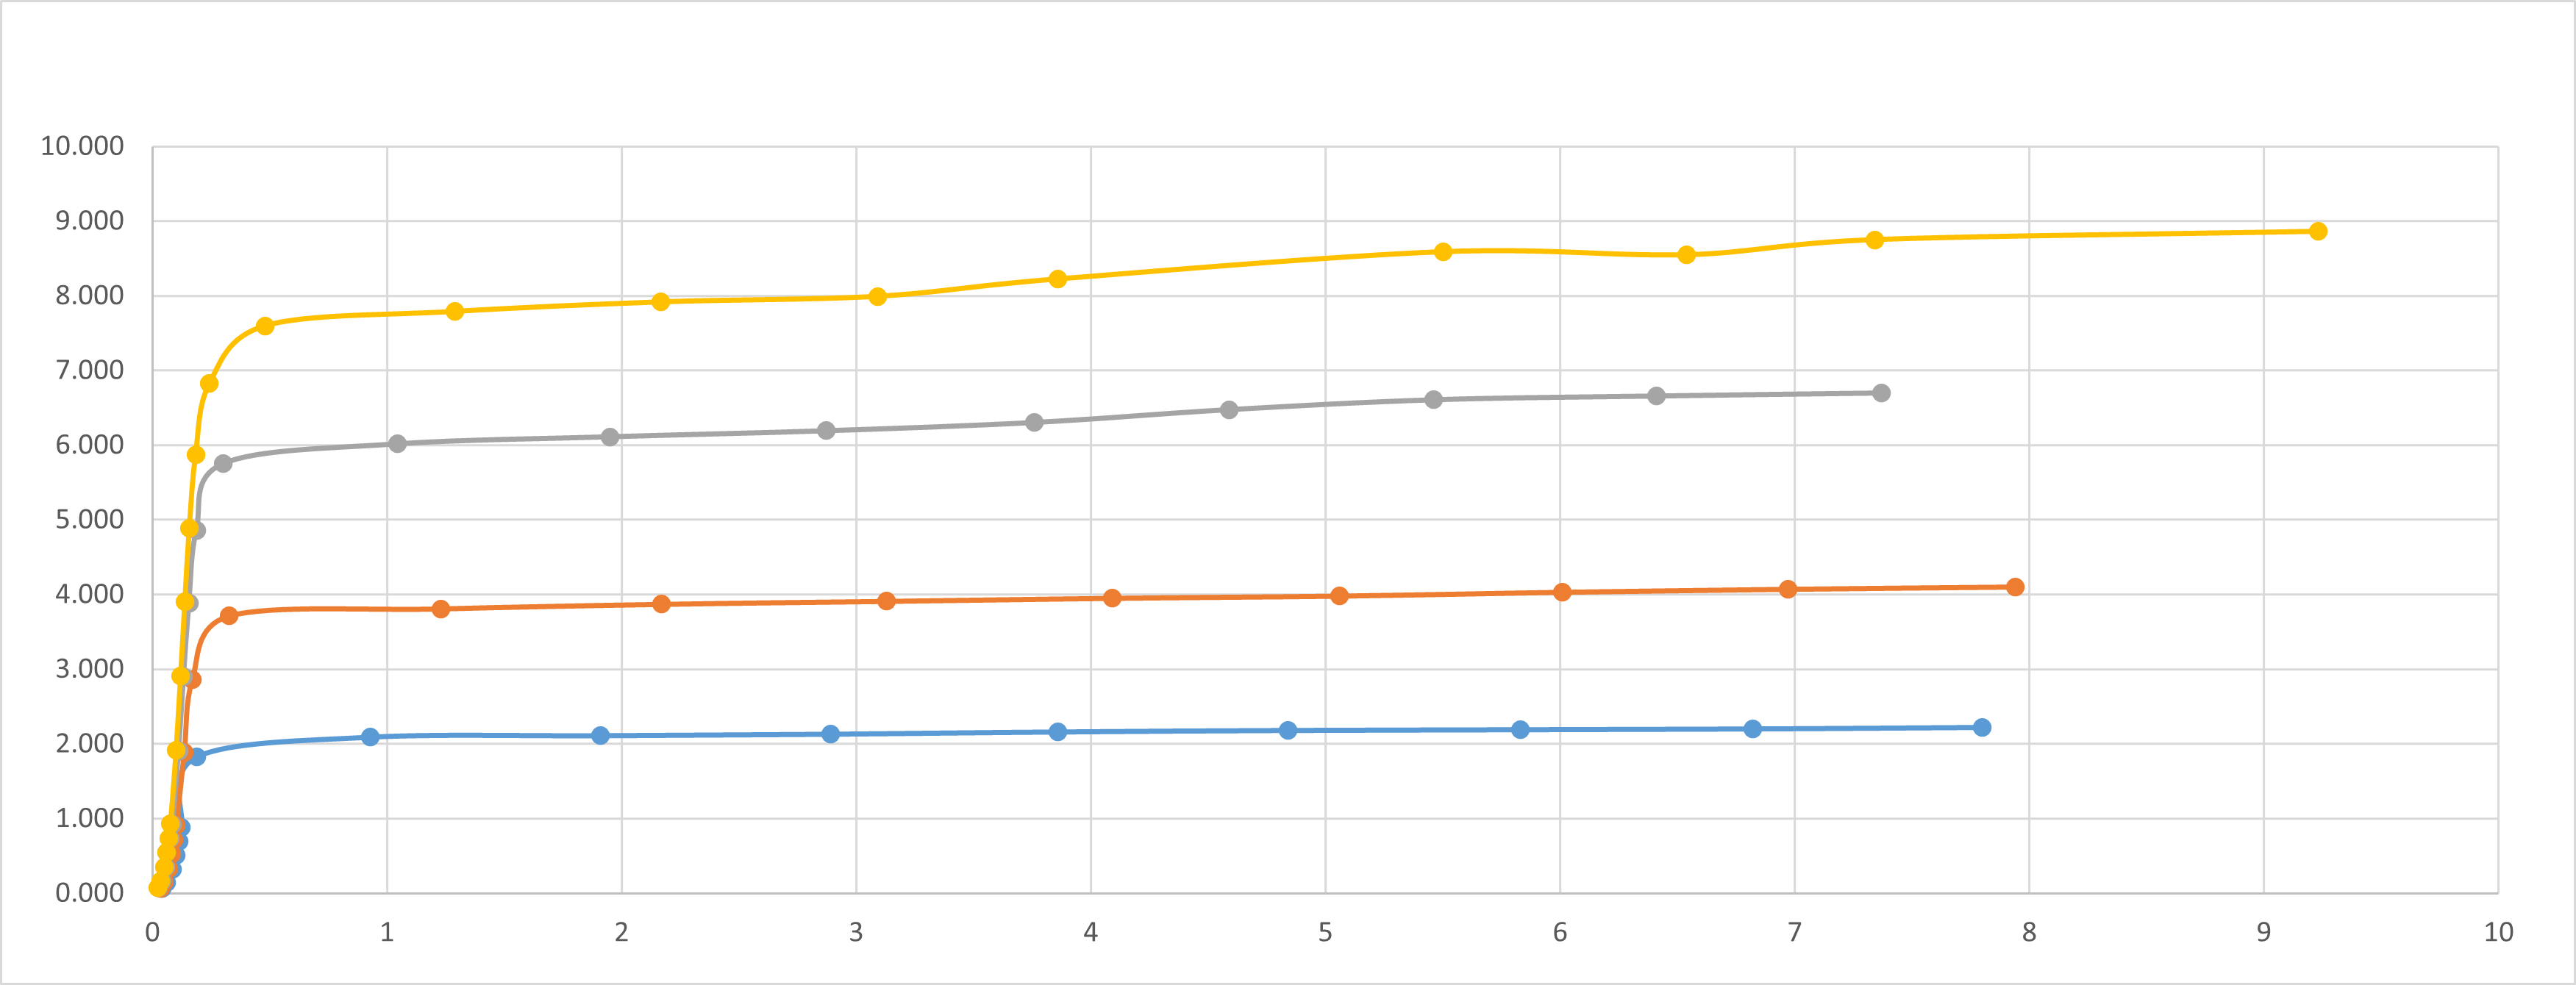
\includegraphics[width=0.9\linewidth]{Experiment_04/DataPlots.png}
        \caption{$I_C$ versus $V_{CE}$}
        \label{L4Plots}
    \end{figure}
    In Fig.\ref{L4Plots}, the different colour of curve represents different $V_{BB}$:
    \begin{itemize}
        \item \textbf{Yellow} $V_{BB} = 2.0V$
        \item \textbf{Grey} $V_{BB} = 1.7V$
        \item \textbf{Orange} $V_{BB} = 1.3V$
        \item \textbf{Blue} $V_{BB} = 1.0V$
    \end{itemize}
    With the help of the plot, the boundary point between forward-active and saturation mode of each $V_{BB}$, $V_{CE} \ge 0.2V$:\par
    \begin{itemize}
        \item $V_{BB} = 2.0V$~~~$V_{CC} = 7V$
        \item $V_{BB} = 1.7V$~~~$V_{CC} = 6V$
        \item $V_{BB} = 1.3V$~~~$V_{CC} = 4V$
        \item $V_{BB} = 1.0V$~~~$V_{CC} = 3V$
    \end{itemize}
    And the estimated values of Early voltage $V_A$ and the common-emitter current gain $\beta$ are $-26.95V$ and $335k$, respectively.
    
\subsection{Experiment Conclusion}
    \subsubsection{Conclusion}
    In this experiment, we have learned the basic operation of a BJT transistor, and the relationship between $V_{CE}$ and $I_C$. We have also learned how to estimate the Early voltage $V_A$ and the common-emitter current gain $\beta$ of the BJT transistor. The estimated values of $V_A$ and $\beta$ are $-26.95V$ and $335k$, respectively.
\section{Operation Modes of Bipolar Junction Transistor}

\subsection{Experiment Design}
    \subsubsection{Background}
    There are two types of Bipolar Junction Transistors: NPN type and PNP types. They are difference in structure and have a symetric response to the circuit enviroment.\par

    In this experiment, we are going to learn operation modes of both type of BJT.\par

    \subsubsection{Propose}
    \begin{itemize}
        \item To test the different operation modes of a npn BJT
        \item To test the different operation modes of a pnp BJT
    \end{itemize}

\subsection{Experiment Design}
    \subsubsection{Materials}
        In this experiment, we will use the following components:
        \begin{itemize}
            \item 2N3904\_1 BJT (NPN)
            \item 2N3906\_1 BJT (PNP)
            \item Resistors
            \item Breadboard
            \item DC power supply
            \item Digital Multi-Meter
        \end{itemize}

    \subsubsection{Circuit Diagram}
        The following circuit diagrams 
        \begin{figure}[H]
            \centering
            \begin{subfigure}{0.4\textwidth}
                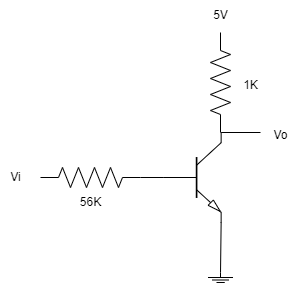
\includegraphics[width=1\linewidth]{Experiment_05/Circuits/Lab5a.png}
                \caption{Circuit for NPN BJT}
                \label{cir:5NPN}
            \end{subfigure}
            \begin{subfigure}{0.4\textwidth}
                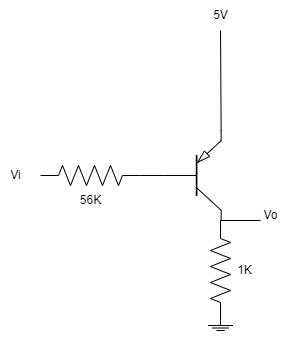
\includegraphics[width=1\linewidth]{Experiment_05/Circuits/Lab5b.png}
                \caption{Circuit for PNP BJT}
                \label{cir:5PNP}
            \end{subfigure}
            \caption{Minimal working Circuit for NPN and PNP BJT}
        \end{figure}

    \subsubsection{Theoretical Analysis}
        \begin{enumerate}[a]
            \item \textbf{The NPN BJT}\par
                NPN BJT have one P-type semi-conductor between two layers of N-type semi-conductor, and therefore it work in forward-biased when the base is positive.\par 
                Because of the symetric of two types of BJT, the NPN BJT will work in the opposite way of the PNP BJT, and here we will analyze the circuit of NPN BJT in figure \ref{cir:5NPN}.\par
        
                The $I_B$ can we express by KVL:
                \begin{equation}
                    I_B =
                        \begin{cases} 
                            0, & V_i < 0.6 \, \text{V} \, \text{(cutoff)} \\ 
                            \frac{V_i - 0.6}{R_B}, & V_i \geq 0.6 \, \text{V} \, \text{(active or saturation)}
                        \end{cases}
                \end{equation}
        
                Then, we can calculate the collector current
                \begin{equation}
                    I_C =
                    \begin{cases}
                        0, & \text{cutoff region} \\ 
                        \beta I_B, & \text{forward-active region (unsaturated)}
                    \end{cases}
                \end{equation}
        
                The output voltage can be calculated as 
                \begin{equation}
                    V_o =
                    \begin{cases}
                        5 \, \text{V}, & V_i < 0.6 \, \text{V} \\ 
                        5 \, \text{V} - I_C R_C, & 0.6 \, \text{V} < V_i < 1.944 \, \text{V} \\ 
                        V_{CE,\text{sat}} \approx 0.2 \, \text{V}, & V_i \geq 1.944 \, \text{V}
                    \end{cases}
                \end{equation}
        
            \item \textbf{The PNP BJT}\par
                PNP BJT have one N-type semi-conductor between two layers of P-type semi-conductor, and therefore it work in forward-biased when the base is negative.\par

                For the PNP BJT, the operation modes are the same as the NPN BJT, but the direction of the current and voltage are opposite, which is:
                \begin{equation}
                    V_o =
                        \begin{cases}
                            0, & V_i > 4.4 \, \text{V} \\ 
                            I_C R_C, & 3.056 \, \text{V} < V_i \leq 4.4 \, \text{V} \\ 
                            5 - V_{CE,\text{sat}} \approx 4.8 \, \text{V}, & V_i \leq 3.056 \, \text{V}
                        \end{cases}
                \end{equation}
        
        \end{enumerate}


\subsection{Experiment record}
    \subsubsection{NPN BJT}
    \begin{enumerate}[I]
        \item \textbf{Data Recorded}\newline
            The recorded data for the integration operation circuit is shown in the following table:
            \begin{table}[H]
                \centering
                \begin{tabular}{|c|c|c|c|c|c|c|c|c|c|}
                    \hline
                    Vi   & 0    & 0.25 & 0.5   & 0.6   & 0.75  & 0.82  & 1     & 1.5   & 1.6   \\ \hline
                    Vo   & 4.91 & 4.91 & 4.91  & 4.78  & 4.22  & 3.85  & 2.25  & 0.24  & 0.24  \\ \hline
                    Theo & 5    & 5    & 5     & 5     & 4.46  & 4.21  & 3.57  & 0.2   & 0.2   \\ \hline
                    Vi   & 1.65 & 1.7  & 1.75  & 1.8   & 1.9   & 2     & 3     & 4     & 5     \\ \hline
                    Vo   & 0.21 & 0.2  & 0.191 & 0.181 & 0.171 & 0.163 & 0.123 & 0.106 & 0.095 \\ \hline
                    Theo & 0.2  & 0.2  & 0.2   & 0.2   & 0.2   & 0.2   & 0.2     & 0.2     & 0.2     \\ \hline
                \end{tabular}
                \caption{Recorded Data for NPN BJT}
                \label{tab:}
            \end{table}
        \item \textbf{Data Analysis}\newline
            The expected output voltage is calculate using the theoretical analysis, and the result is shown in the table above. From the table we can see that the output voltage is close to the theoretical value, so our experiment is successful.
    \end{enumerate}

    \subsubsection{PNP BJT}
    \begin{enumerate}[I]
        \item \textbf{Data Recorded}\newline
            The recorded data for the integration operation circuit is shown in the following table:
            \begin{table}[H]
                \centering
                \begin{tabular}{|c|c|c|c|c|c|c|c|c|c|}
                    \hline
                    Vi   & 0    & 0.65 & 1.41 & 2.09 & 2.48 & 2.98  & 3.13  & 3.26 & 3.48 \\ \hline
                    Vo   & 4.83 & 4.82 & 4.81 & 4.79 & 4.77 & 4.8  & 4.09  & 3.69 & 3    \\ \hline
                    Theo & 4.8  & 4.8  & 4.8  & 4.8  & 4.8  & 5.10  & 4.56  & 4.09 & 3.30 \\ \hline
                    Vi   & 3.61 & 3.76 & 3.92 & 4.06 & 4.19 & 4.21  & 4.49  & 5    &      \\ \hline
                    Vo   & 2.55 & 2.04 & 1.5  & 1.03 & 0.65 & 0.587 & 0.004 & 0    &      \\ \hline
                    Theo & 2.84 & 2.30 & 1.72 & 1.22 & 0.75 & 0.68  & 0     & 0    &      \\ \hline
                \end{tabular}
                \caption{Recorded Data for PNP BJT}
                \label{tab:}
            \end{table}
        \item \textbf{Data Analysis}\newline
            The expected output voltage is calculate using the theoretical analysis, and the result is shown in the table above. From the table we can see that the output voltage is close to the theoretical value, so our experiment is successful.
    \end{enumerate}
    
\subsection{Experiment Conclusion}
    \subsubsection{Conclusion}
    In this experiment, we have learned the operation modes of both NPN and PNP BJT. We have tested the circuit of both type of BJT, and observe the citcuit behaive in three different operation mode.
\section{Common\-Emitter BJT Amplifier}

\subsection{Experiment Design}
    \subsubsection{Background}
    In this experiment, we want to measure the quiescent-point of a common-emitter BJT amplifier and evaluate the small-signal amplification function of a common-emitter amplifier.\par

    The Common\-Emitter have the property of high input impedence and high voltage gain.\par

    \subsubsection{Propose}
    \begin{itemize}
        \item To measure the quiescent-point of a common-emitter BJT amplifier
        \item To evaluate the small-signal amplification function of a common-emitter amplifier
    \end{itemize}

\subsection{Experiment Design}
    \subsubsection{Materials}
        In this experiment, we will use the following components:
        \begin{itemize}
            \item 2N3904\_1 BJT
            \item Resistors
            \item Capacitors
            \item DC power supply
            \item Digital Multi-Meter
            \item Function Generator
            \item Oscilloscope
        \end{itemize}

    \subsubsection{Circuit Diagram}
        The following circuit diagrams 
        \begin{figure}[H]
            \centering
            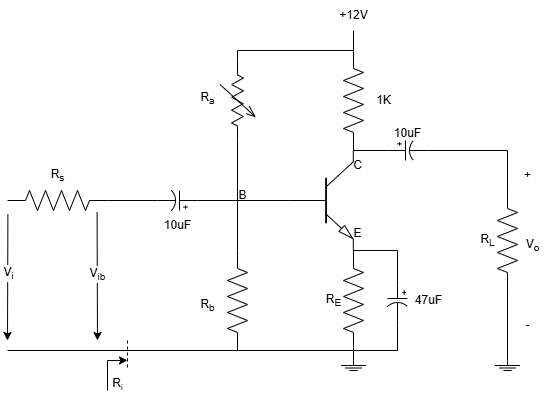
\includegraphics[width=0.5\linewidth]{Experiment_06/Circuit/Lab6.drawio.png}
            \caption{Common\-Emitter BJT Amplifier}
            \label{cir:6main}
        \end{figure}

    \subsubsection{Theoretical Analysis}
        \begin{enumerate}[I]
            \item \textbf{DC Analysis}
                First, we analyze the circuit by drawing its DC-equivalent circuit to find its quiescent working point.\par
                \begin{figure}[H]
                    \centering
                    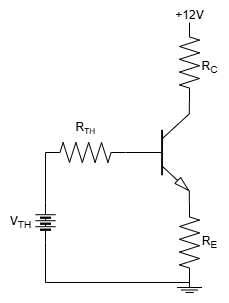
\includegraphics[width=0.3\linewidth]{Experiment_06/Circuit/Lab6dc.drawio.png}
                    \caption{DC-equivalent Circuit}
                    \label{cir:6dc}
                \end{figure}
                In Fig.\ref{cir:6dc}, we can obtain the value of $R_{TH}$ and $V_{TH}$
                \begin{equation}
                    R_{\text{TH}} = R_a \parallel R_b, \quad V_{\text{TH}} = V \frac{R_b}{R_a + R_b}
                \end{equation}
                Then, we can calculate the value of $I_{\text{CQ}}$ and $V_{\text{CEQ}}$ by using the following equations:
                \begin{equation}
                    I_C = \beta I_B, \quad I_E = (1 + \beta) I_B, \quad V_C = 12 - I_C R_C, \quad V_B = V_{\text{TH}} - I_B R_B
                \end{equation}
                Finally, we can derive the value of $I_{\text{CQ}}$ and $V_{\text{CEQ}}$ by using the following equations:
                \begin{equation}
                    V_{\text{TH}} - I_B R_{\text{TH}} - V_{BE} - I_E R_E = 0, \quad I_B = \frac{V_{\text{TH}} - V_{BE}}{R_{\text{TH}} + (1+\beta)R_E}
                \end{equation}
            \item \textbf{AC Analysis}
                Next, we analyze the circuit by drawing its AC-equivalent circuit to find its small-signal amplification function.\par
                \begin{figure}[H]
                    \centering
                    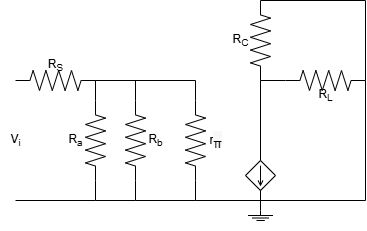
\includegraphics[width=0.5\linewidth]{Experiment_06/Circuit/Lab6ac.drawio.png}
                    \caption{AC-equivalent Circuit}
                    \label{cir:6ac}
                \end{figure}
                In Fig.\ref{cir:6ac}, we can calculate the theoretical value of $V_O and V_i$, as well as the output and input impedence.
                \begin{equation*}
                    V_o = \beta i_B (R_C \parallel R_L)
                \end{equation*}
                \begin{equation*}
                    V_i = i_B r_\pi + \left(\frac{i_B r_\pi}{R_a} + \frac{i_B r_\pi}{R_b} + i_B \right) R_S
                \end{equation*}
                \begin{equation*}
                    R_i = R_a \parallel R_b \parallel r_\pi, 
                    \quad 
                    R_o = R_C \parallel R_L
                \end{equation*}
        \end{enumerate}

\subsection{Experiment record}
    \subsubsection{DC Analysis}
    Set $v_i$ euqals to zero, we can obtain the following data:
    \begin{table}[H]
        \centering
            \begin{tabular}{|l|ccccccc|}
            \hline
            & $V_B$ & $V_C$  & $V_E$ & $I_B$ & $I_C$  & $I_E$  & $\beta$ \\ \hline
            Meas & 3.776 & 10.435 & 3.118 & 12.3u & 1.565m & 1.553m & 127     \\ \hline
            Theo & 3.903 & 10.47  & 3     & 9.56u & 1.533m & 1.539m & 160     \\ \hline
        \end{tabular}
        \caption{Measured Data of DC Analysis}
        \end{table}
    From the table, we can see our theoretical data is close to the measured data, which means our theoretical analysis is correct.

    \subsubsection{AC Analysis}
    We adjust our $v_i$ in a rage that not distrot the output signal, and we can obtain the following data:
    \begin{table}[H]
        \centering
            \begin{tabular}{|l|cccc|}
            \hline
            $v_{ib}$ & 5.5  & 8.25 & 11   & 13.4 \\ \hline
            $v_o$    & 212  & 317  & 422  & 605  \\ \hline
            $A_v$    & 38.5 & 38.4 & 38.4 & 45.1 \\ \hline
        \end{tabular}
        \caption{Measured Data of AC Analysis}
    \end{table}

    And here is the plot output of the AC Analysis:
    \begin{figure}[H]
        \centering
        \begin{subfigure}{0.25\textwidth}
            \centering
            \includegraphics[width = 1\linewidth]{Experiment_06/Images/6.6_Vi-Vib_a.jpg}
            \caption{1000Hz, 0.5V peak}
            \label{l6acvg}
        \end{subfigure}
        \begin{subfigure}{0.25\textwidth}
            \centering
            \includegraphics[width=1\linewidth]{Experiment_06/Images/6.5_Vo-Vib_distrupted.jpg}
            \caption{Disrupted Waveform}
            \label{l6dcdisrupted}
        \end{subfigure}
        \begin{subfigure}{0.25\textwidth}
            \centering
            \includegraphics[width=1\linewidth]{Experiment_06/Images/6.5_Vo-Vib_025mV.jpg}
            \caption{0.025V Waveform}
            \label{l6dc025}
        \end{subfigure}

        \begin{subfigure}{0.25\textwidth}
            \centering
            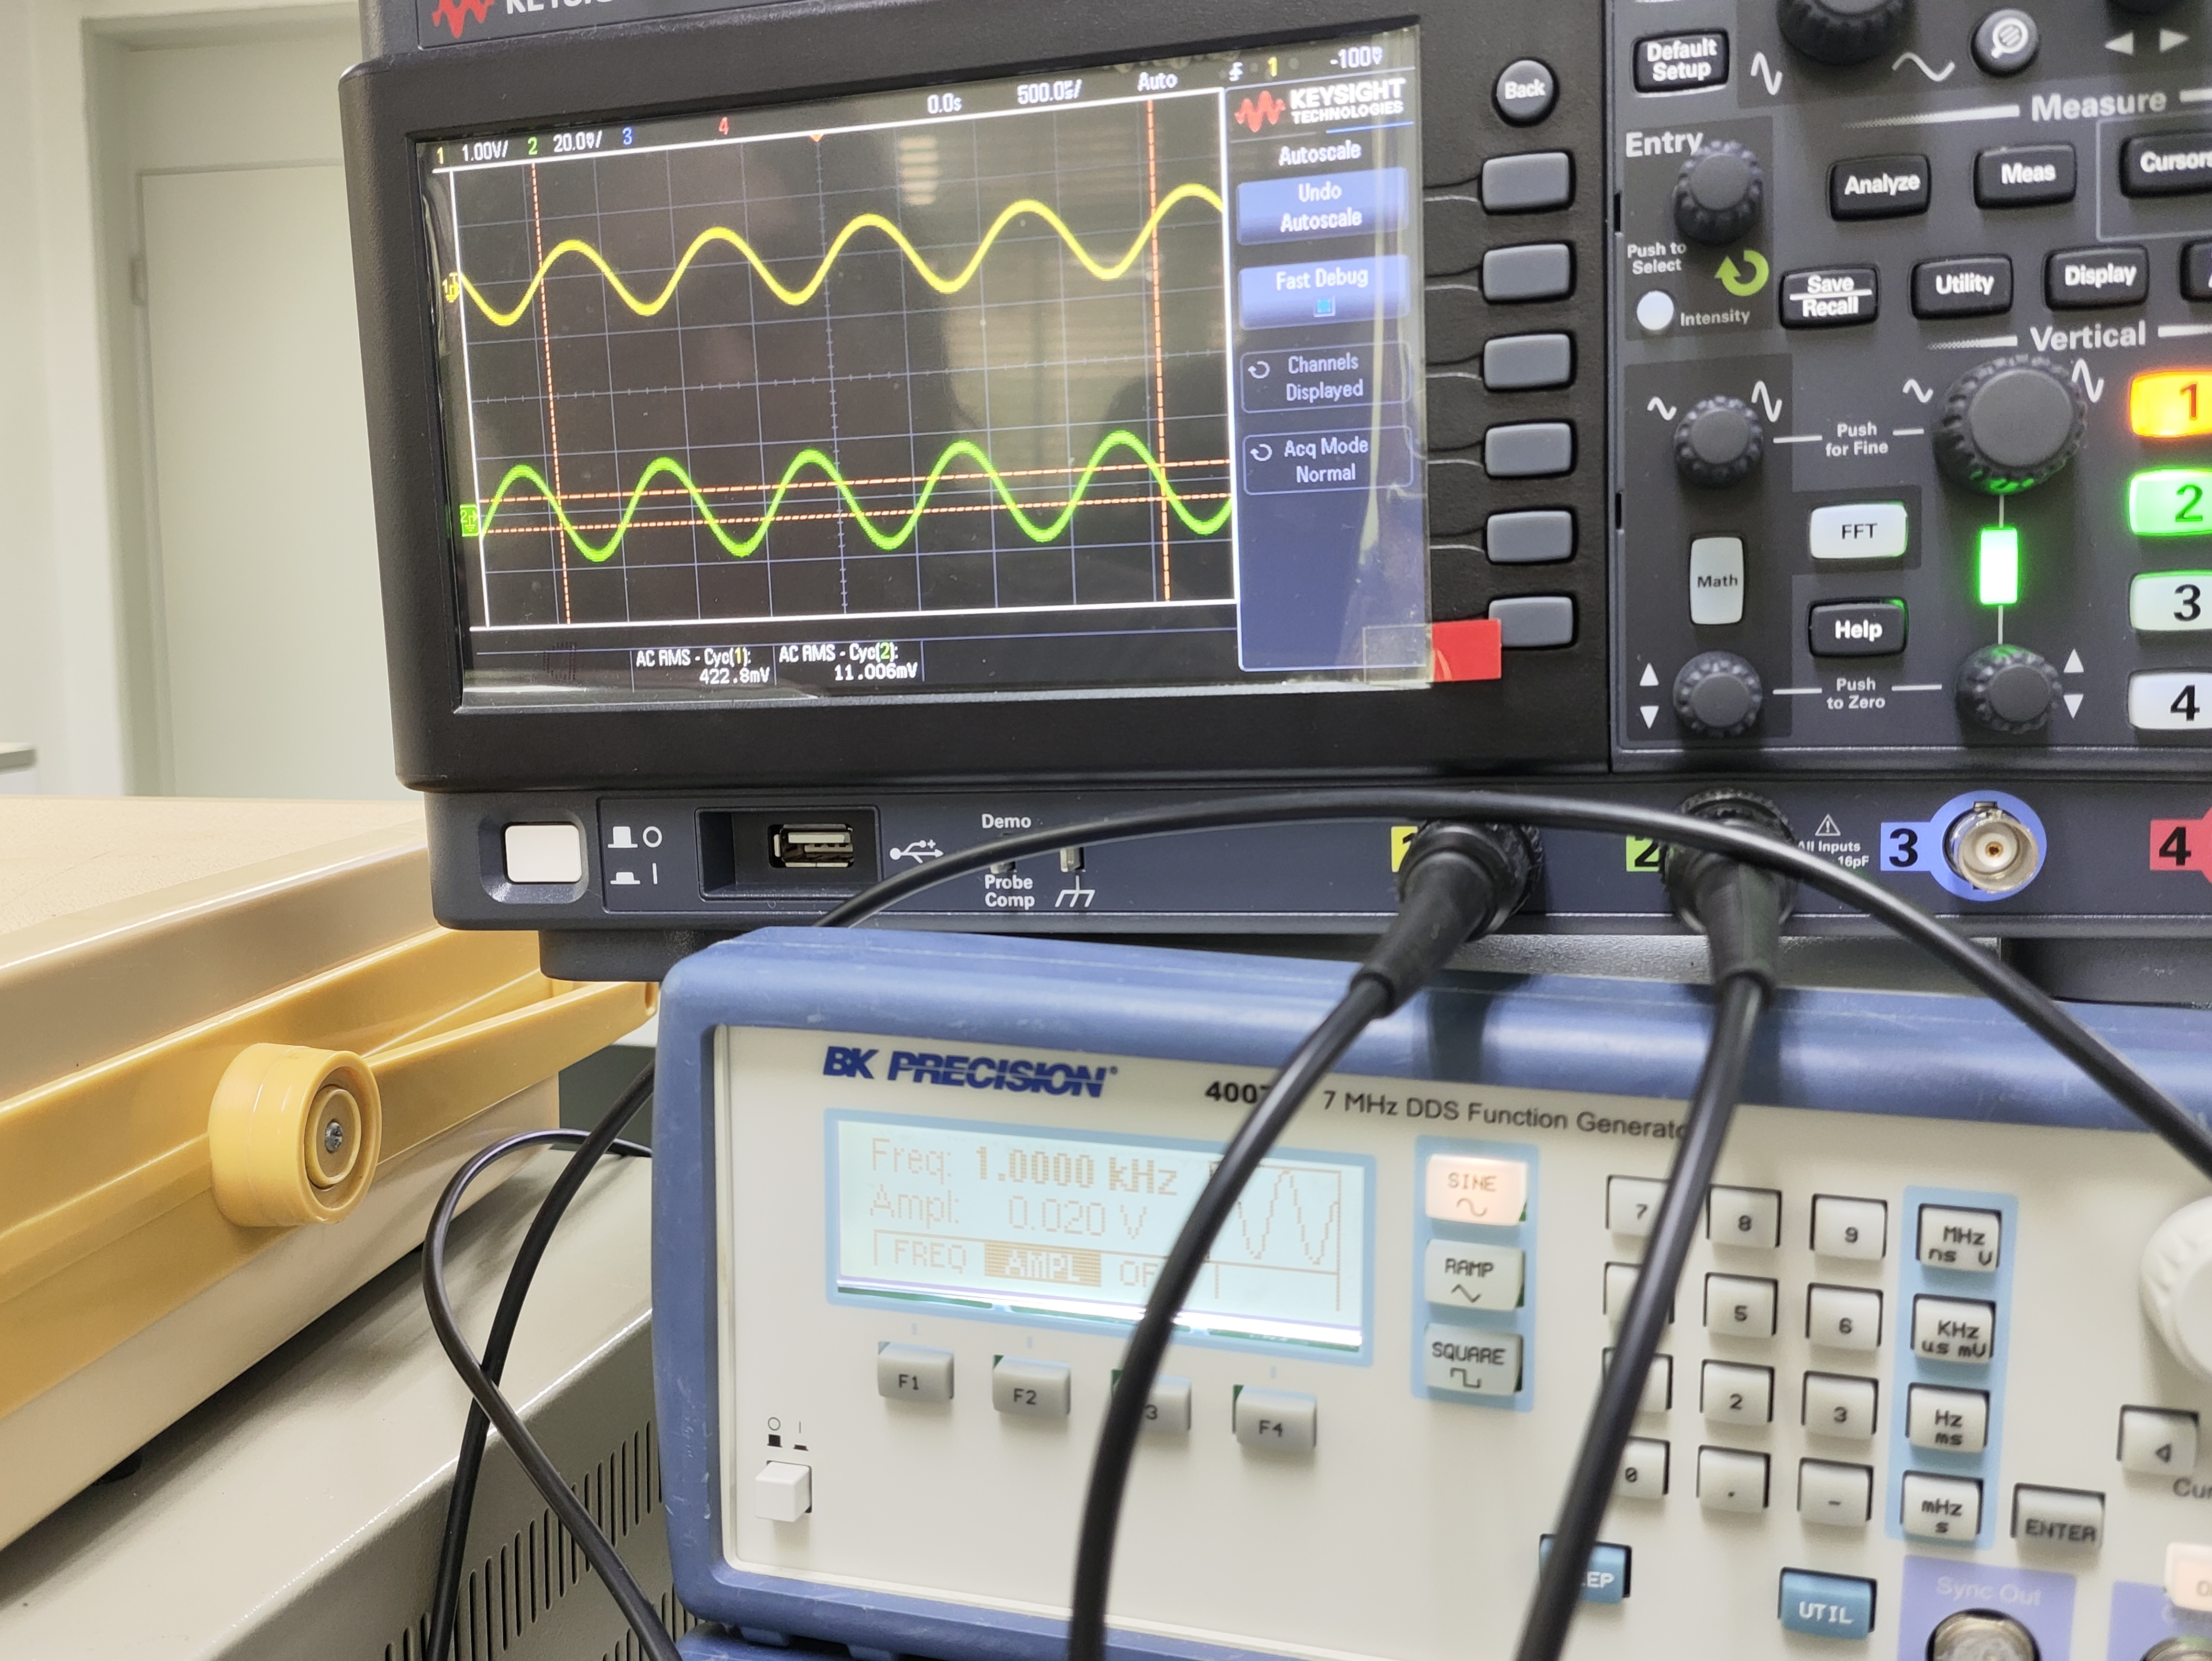
\includegraphics[width=1\linewidth]{Experiment_06/Images/6.5_Vo-Vib_020mV.jpg}
            \caption{0.020V Waveform}
            \label{l6dc020}
        \end{subfigure}
        \begin{subfigure}{0.25\textwidth}
            \centering
            \includegraphics[width=1\linewidth]{Experiment_06/Images/6.5_Vo-Vib_015mV.jpg}
            \caption{0.015V Waveform}
            \label{l6acvg015}
        \end{subfigure}
        \begin{subfigure}{0.25\textwidth}
            \centering
            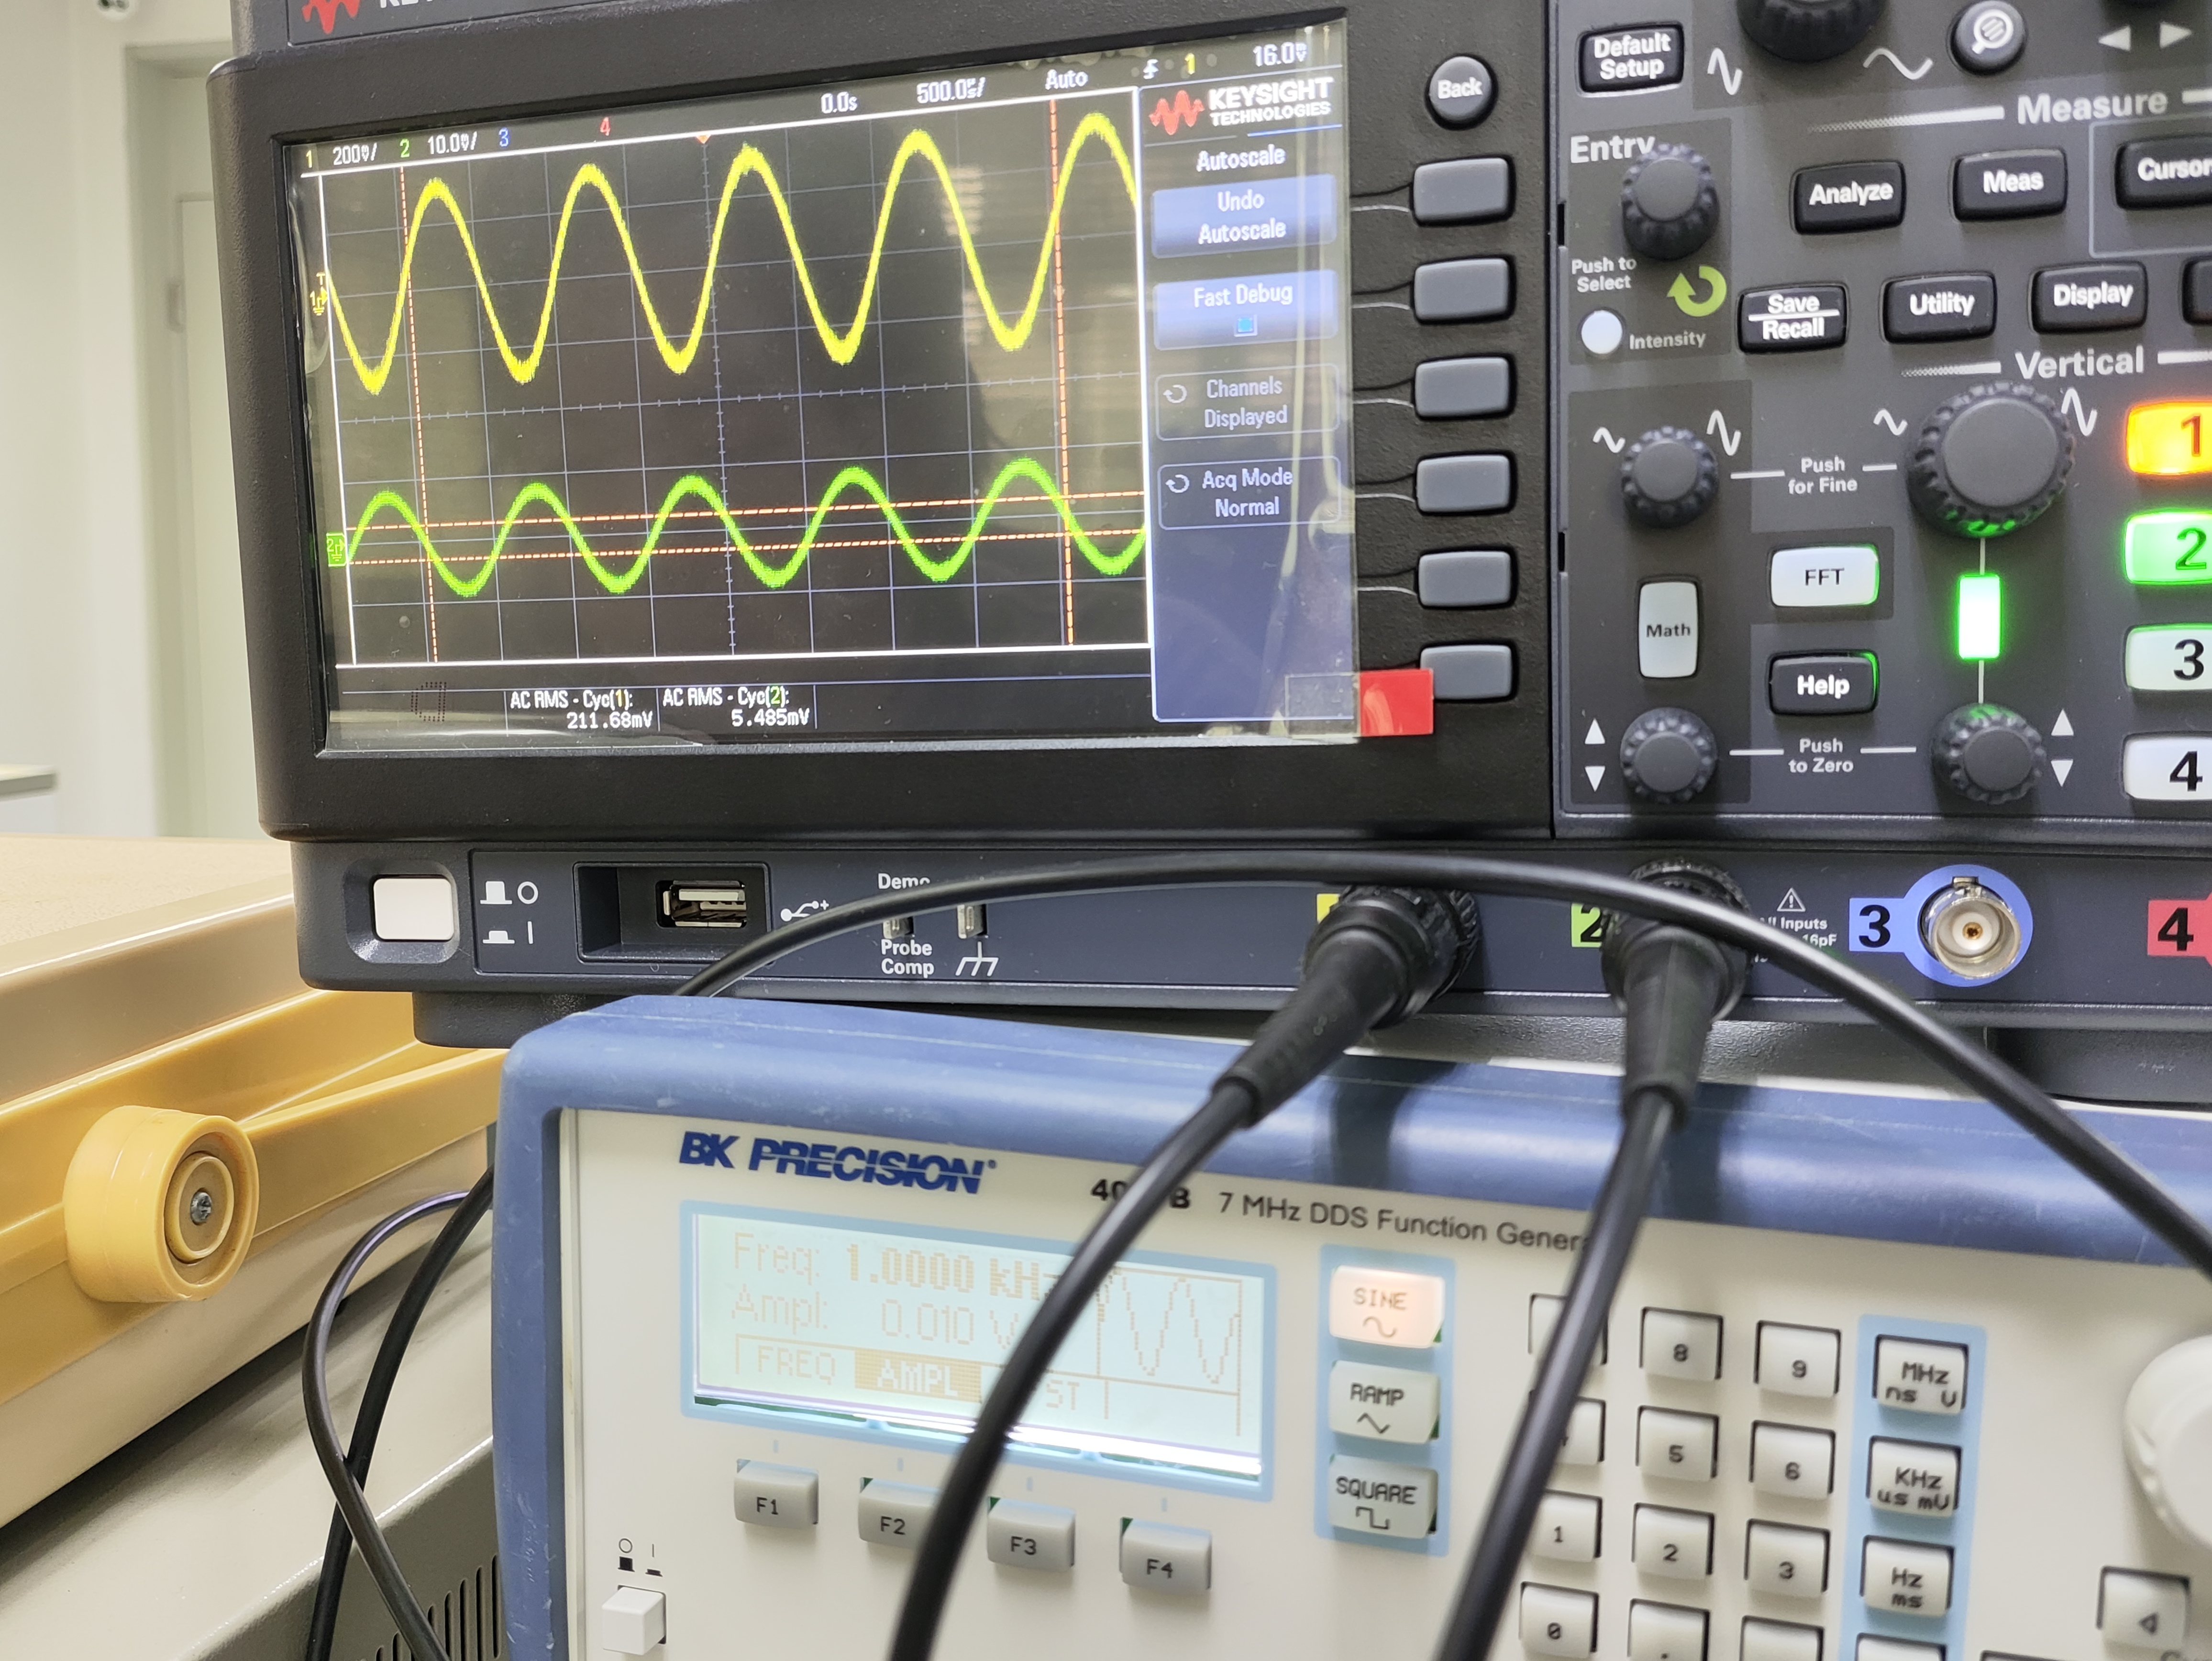
\includegraphics[width=1\linewidth]{Experiment_06/Images/6.5_Vo-Vib_010mV.jpg}
            \caption{0.10V Waveform}
            \label{l6acvg010}
        \end{subfigure}
    \end{figure}

    Finally, we can find the input and output impedence of the circuit by using the following equations:
    ($V^*$ = 0.025 V for Input, $V^*$ = 0.160 V for Output)\par
    \begin{table}[H]
    \centering
        \begin{tabular}{l|c}
        \hline
        $v_i=18.1mV$ & $V_{ib}=13.7mV$ \\
        $v_i=10.8mV$ & $V_{ib}= 8.2mV$  \\
        $v_i=7.24mV$ & $V_{ib}=5.48mV$ \\
        \end{tabular}
        \caption{Various Input voltage and $V_{ib}$}
    \end{table}
    From this, we can calculate the input impedence, which is 
    \begin{equation}
        R_i = 13.55k \Omega
    \end{equation}

    \begin{table}[H]
        \centering
            \begin{tabular}{l|c}
            \hline
            $R_L$ & $V_O$ \\
            $300k \Omega$ & $0.219V$ \\
            $2k \Omega$ & $0.393V$ \\
            \end{tabular}
        \end{table}
    From this, we can calculate the output impedence, which is
    \begin{equation}
        R_o = 0.982k \Omega
    \end{equation}
\subsection{Experiment Conclusion}
    \subsubsection{Conclusion}
    In this experiment, we have successfully measured the quiescent-point of a common-emitter BJT amplifier and evaluated the small-signal amplification function of a common-emitter amplifier. We have also calculated the input and output impedence of the circuit.
\section{The Common\-Collector BJT Amplifier}

\subsection{Experiment Design}
    \subsubsection{Background}
    An Amlifier is a device that can increase the power of a signal.
    And a Common\-Collector BJT Amplifier have the characters of high input impedance and low output impedance.
    It can be used as a buffer to isolate the input and output impedance of the circuit.\par

    \subsubsection{Propose}
    \begin{itemize}
        \item Measure the quiescent-point of an emitter follwer(CC Amplifier)
        \item Ecaluate the small-signal amplification function of an emitter follower
    \end{itemize}

\subsection{Experiment Design}
    \subsubsection{Materials}
        In this experiment, we will use the following components:
        \begin{itemize}
            \item 2N3904\_1
            \item Capacitors
            \item Resistors
            \item DC Power Supply
            \item Function Generator
            \item Oscilloscope
            \item Digital Multimeter
        \end{itemize}
    \subsubsection{Circuit Diagram}
        The circuit diagram of the Common\-Collector BJT Amplifier is shown in Figure \ref{fig:CC_Amplifier}.
        \begin{figure}[H]
            \centering
            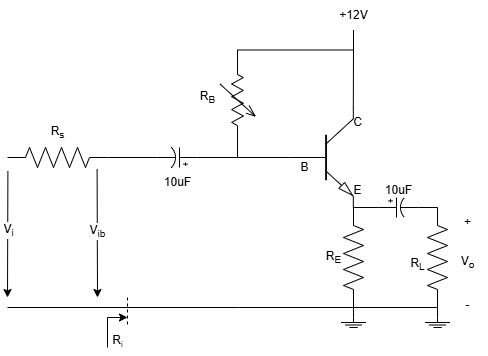
\includegraphics[width=0.5\linewidth]{Experiment_07/Circuit/Lab7.drawio.png}
            \caption{Common\-Collector BJT Amplifier}
        \end{figure}

    \subsubsection{Theoretical Analysis}

    \begin{enumerate}[I]
        \item \textbf{DC Analysis}
            First, we analyze the circuit by drawing its DC-equivalent circuit to find its quiescent working point.\par
            \begin{figure}[H]
                \centering
                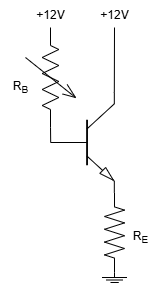
\includegraphics[width=0.2\linewidth]{Experiment_07/Circuit/Lab7dc.drawio.png}
                \caption{DC-equivalent Circuit}
                \label{cir:7dc}
            \end{figure}
            In Fig.\ref{cir:7dc}, we can obtain the expression of some basic current.
            \begin{equation}
                V_{CC} - i_B R_B - V_{BE} - (1+\beta) i_B R_E = 0, \quad
                i_B = \frac{V_{CC} - V_{BE}}{R_B + (1+\beta) R_E}     
            \end{equation}
        \item \textbf{AC Analysis}
            Next, we analyze the circuit by drawing its AC-equivalent circuit to find its small-signal amplification function.\par
            \begin{figure}[H]
                \centering
                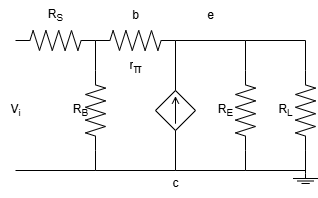
\includegraphics[width=0.5\linewidth]{Experiment_07/Circuit/Lab7ac.drawio.png}
                \caption{AC-equivalent Circuit}
                \label{cir:7ac}
            \end{figure}
            In Fig.\ref{cir:7ac}, we can obtain the expression of the voltage gain, input impedance, and output impedance.
            \begin{itemize}
                \item \textbf{Input output voltage:}
                \[
                    V_o = (R_E \parallel R_L)(1+\beta) i_B, \quad
                    V_i = i_B r_\pi + V_o + R_S \left(i_B + \frac{i_B r_\pi + V_o}{R_B}\right)
                \]
                \item \textbf{Voltage gain:}
                \[
                    A_V = \frac{V_o}{V_i}
                \]
                \item \textbf{Input and Output impedance:}
                \[
                    R_i = \frac{i_B r_\pi + V_o}{\frac{i_B}{R_B} + \frac{1}{R_S}}, \quad
                    R_o = \frac{V_x}{i_x}
                \]
                where $V_x$ and $i_x$ is given by the following equation:
                \[
                    I_x + (1+\beta)i_B = \frac{V_x}{R_E \parallel R_L}, \quad
                    V_x + i_B r_\pi + i_B(R_S \parallel R_B)
                \]
            \end{itemize}
    \end{enumerate}

\subsection{Experiment record}
\subsubsection{DC Analysis}
Set $v_i$ as zero, and we can measure the terminal voltage of the BJT\\
    \begin{equation}
    \centering
            V_B =10.10,\quad
            V_C =12.00,\quad
            V_E =9.505
            \label{eq:7demeas}
    \end{equation}
    Plug equation \ref{eq:7demeas} into the theoretical euquation we obtained above, we can obtain:

        \begin{align*}
            I_{BQ} & = \frac{V_C-V_B}{R_B}=33.929\mu A\\
            I_{EQ} & = \frac{V_E}{R_E}=9.505mA\\
            I_{CQ} & = I_{EQ}-I_{BQ}=9.471mA\\
            \beta  & = 279.14
        \end{align*}


\subsubsection{AC Analysis}
\begin{itemize}
    \item Voltage Gain: Let $v_i$ to be a sinusoidal signal (1000 Hz, 5V peak) and $R_L$ = 300k$\Omega$.
        \begin{table}[h]
        \centering
        \begin{tabular}{l|cccc}
            \toprule
            Vib & 0.9372     & 0.7239      & 0.4901    & 0.24     \\ 
            Vo  & 0.9425     & 0.7072      & 0.4824    & 0.2411   \\
            \midrule
            Av  & 1.00565514 & 0.976930515 & 0.9842889 & 1.004583 \\ 
            \bottomrule
        \end{tabular}
        \caption{Voltage Gain}
        \end{table}
        \FloatBarrier
        When the BJT turns to saturation, the distortion occurs. $R_B$ should be increased to enlarge the linear amplification range.
    \item Input \& Output Resistance: Let $v_i$ to be  a 1000 Hz sinusoidal signal with the amplitude of 1 V.
        The input and output resistance is calculated as the following:
        \begin{equation}
            R_i = \frac{v_{ib} R_S}{v_i-v_{ib}} = \frac{10K * 0.578}{1.15 - 0.578} = 10104.9\Omega
        \end{equation}

        
\end{itemize}

        %\item \textbf{Real Output Impedance}\par
        %    First, we assumet the open-circuit voltage gain is $V_{oc}$, then, we can write the output voltage with load as the following:
        %    \begin{equation}
        %            V_{L1} = V_{OC} \cdot \frac{R_{L1}}{Z_{out} + R_{L1}}
        %    \end{equation}
        %    \begin{equation}
        %            V_{L2} = V_{OC} \cdot \frac{R_{L2}}{Z_{out} + R_{L2}}
        %    \end{equation}
        %    Then, we can get emilate the $V_{oc}$, and find the expression of the output impedance as the following:
        %    \begin{equation}
        %        Z_{out} = \frac{R_{L1} \cdot R_{L2} \cdot (V_{L1} - V_{L2})}{V_{L2} \cdot R_{L1} - V_{L1} \cdot R_{L2}}
        %    \end{equation}

        %    Substitude the value of $V_{L1}$ and $V_{L2}$ for resistance $300k\Omega$ and $1k\Omega$ we can calculate the real output impedance of the circuit:

        %    \begin{equation}
        %        Z_{out} = \frac{300k\Omega \cdot 1k\Omega \cdot (0.588V - 0.568V)}
        %                       {0.568V \cdot300k\Omega -0.588V \cdot 1k\Omega}
        %                = 
        %    \end{equation}
\subsection{Experiment Conclusion}
    \subsubsection{Conclusion}
    In this experiment, we have successfully measured the quiescent-point of an emitter follower(CC Amplifier) and ecaluated the small-signal amplification function of an emitter follower.
    

\section{Properties of a n-channel enhancement MOSEFT}

\subsection{Experiment Design}
    \subsubsection{Propose}
    \begin{itemize}
        \item 2N7000 MOSEFT
        \item Resistors
        \item Capacitors
        \item Breadboard
        \item Oscilloscope
        \item Function Generator
        \item DC Power Supply
        \item Digital Multi-Meter
    \end{itemize}

\subsection{Experiment Design}
    \subsubsection{Materials}
        In this experiment, we will use the following components:
        \begin{itemize}
            \item To find the voltage-current characteristics of a n-channel enhancement MOSFET
            \item To evaluate different operation modes of a n-channel enhancement MOSFET
        \end{itemize}

    \subsubsection{Circuit Diagram}
        The following circuit diagrams 
        \begin{figure}[H]
            \centering
            \begin{subfigure}{0.5\textwidth}
                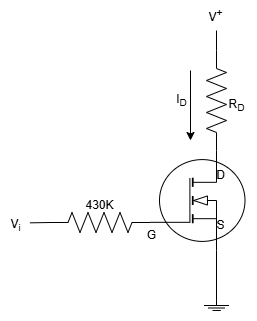
\includegraphics[width=1\linewidth]{Experiment_08/Circuit/Lab8.drawio.png}
                \caption{MOSEFT Circuit}
                \label{cir:8}
            \end{subfigure}
            \caption{}
        \end{figure}


\subsection{Experiment record}
    \subsubsection{Part I}
    The data we recorded for the MOSEFT circuit is shown in the following table:
    \begin{table}[H]
        \centering
        \resizebox{\columnwidth}{!}{%
        \begin{tabular}{l|ccccccccccc}
        \hline
        $Vi     $ & 0.5         & 0.65        & 0.98        & 1.1         & 1.21        & 1.31     & 1.45     & 1.59     & 1.75     & 1.86     & 1.9      \\
        $V_{DS} $ & 11.7        & 11.79       & 11.78       & 11.79       & 11.77       & 11.73    & 11.49    & 10.65    & 8.05     & 4.9      & 3.89     \\
        $V_{R_D}$ & 0.0055      & 0.005       & 0.0058      & 0.007       & 0.0156      & 0.0502   & 0.292    & 1.17     & 3.79     & 6.95     & 8.1      \\
        $I_D    $ & 1.17021E-05 & 1.06383E-05 & 1.23404E-05 & 1.48936E-05 & 3.31915E-05 & 0.000107 & 0.000621 & 0.002489 & 0.008064 & 0.014787 & 0.017234 \\
        \hline
        \hline
        $Vi      $& 1.94        & 1.96        & 2           & 2.15        & 2.28        & 2.4      & 2.525    & 2.66     & 2.73     & 3.05     & 3.2      \\
        $V_{DS}  $& 2.4         & 1.6         & 0.7         & 0.222       & 0.175       & 0.15     & 0.137    & 0.125    & 0.121    & 0.107    & 0.102    \\
        $V_{R_D} $& 9.45        & 10.05       & 11.2        & 11.77       & 11.82       & 11.848   & 11.86    & 11.87    & 11.87    & 11.89    & 11.89    \\
        $I_D     $& 0.020106383 & 0.021382979 & 0.023829787 & 0.025042553 & 0.025148936 & 0.025209 & 0.025234 & 0.025255 & 0.025255 & 0.025298 & 0.025298 \\
        \end{tabular}%
        }
        \caption{Estimation of parameter for MOSEFT}
        \end{table}
    From this 
    Relationship between $V_{GS}$ and $V_{DS}$:\\
    \begin{figure}[H]
        \centering
        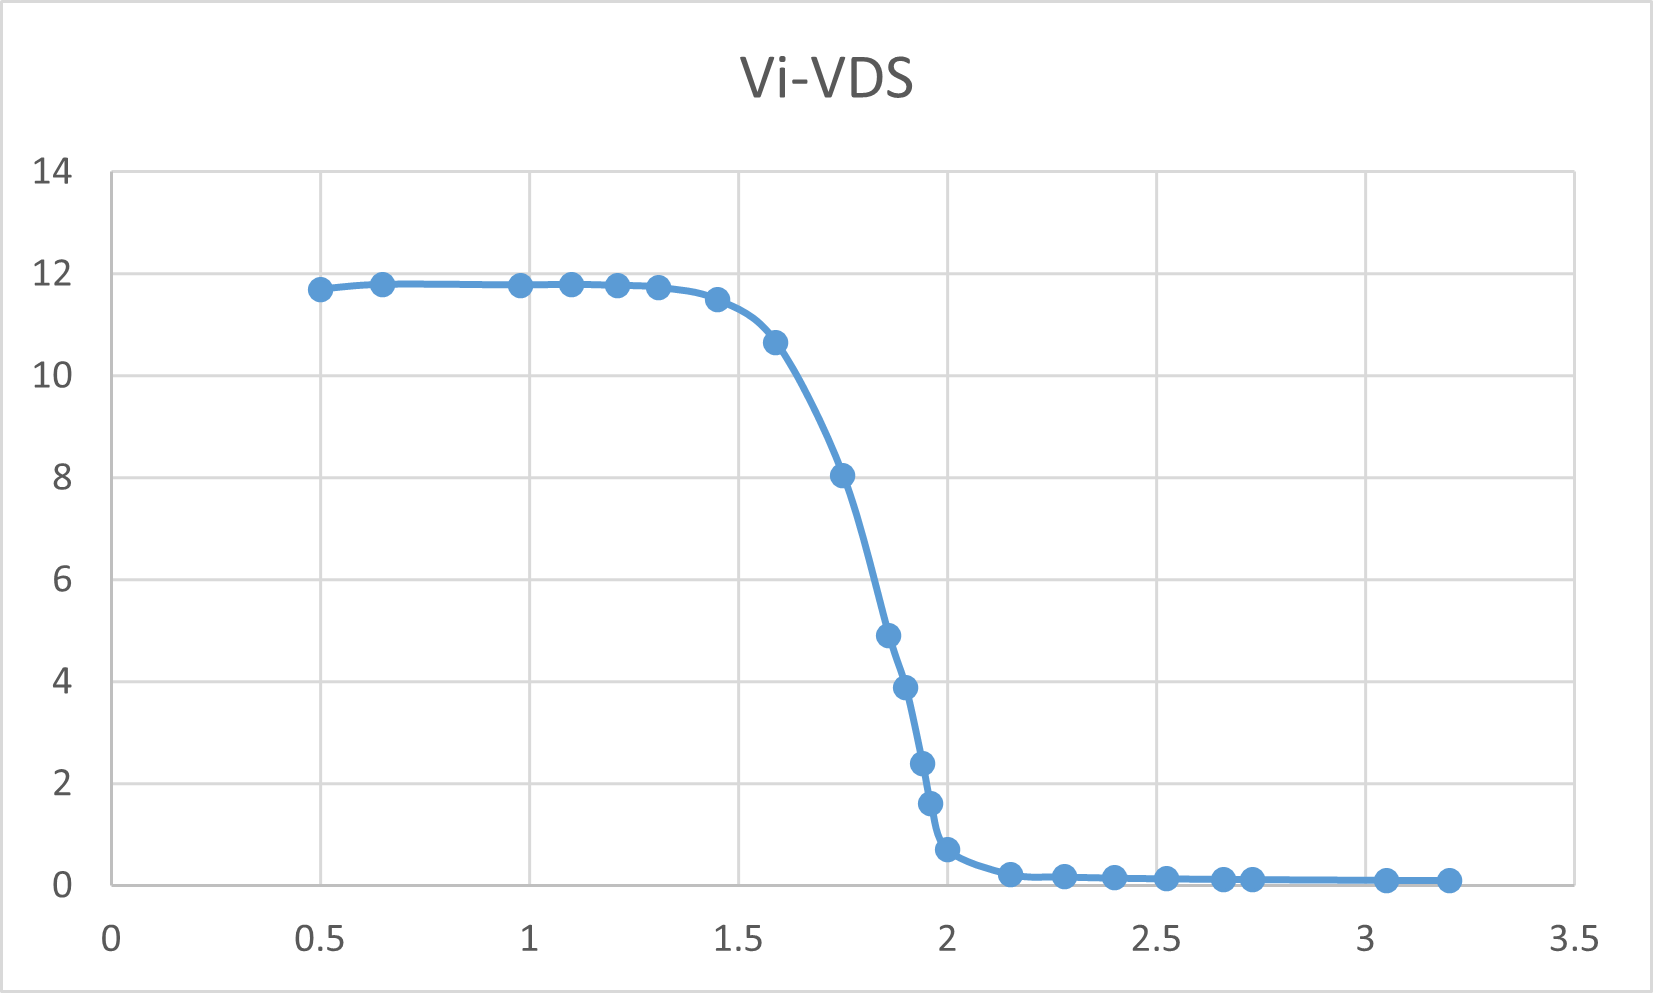
\includegraphics[width=0.5\linewidth]{Experiment_08/Images/L8_DCF1.png}
        \caption{Relationship between $V_{GS}$ and $V_{DS}$}
        \label{l8dctf1}
    \end{figure}
    \FloatBarrier
    Relationship between $V_{GS}$ and $I_D$:\\
    \begin{figure}[H]
        \centering
        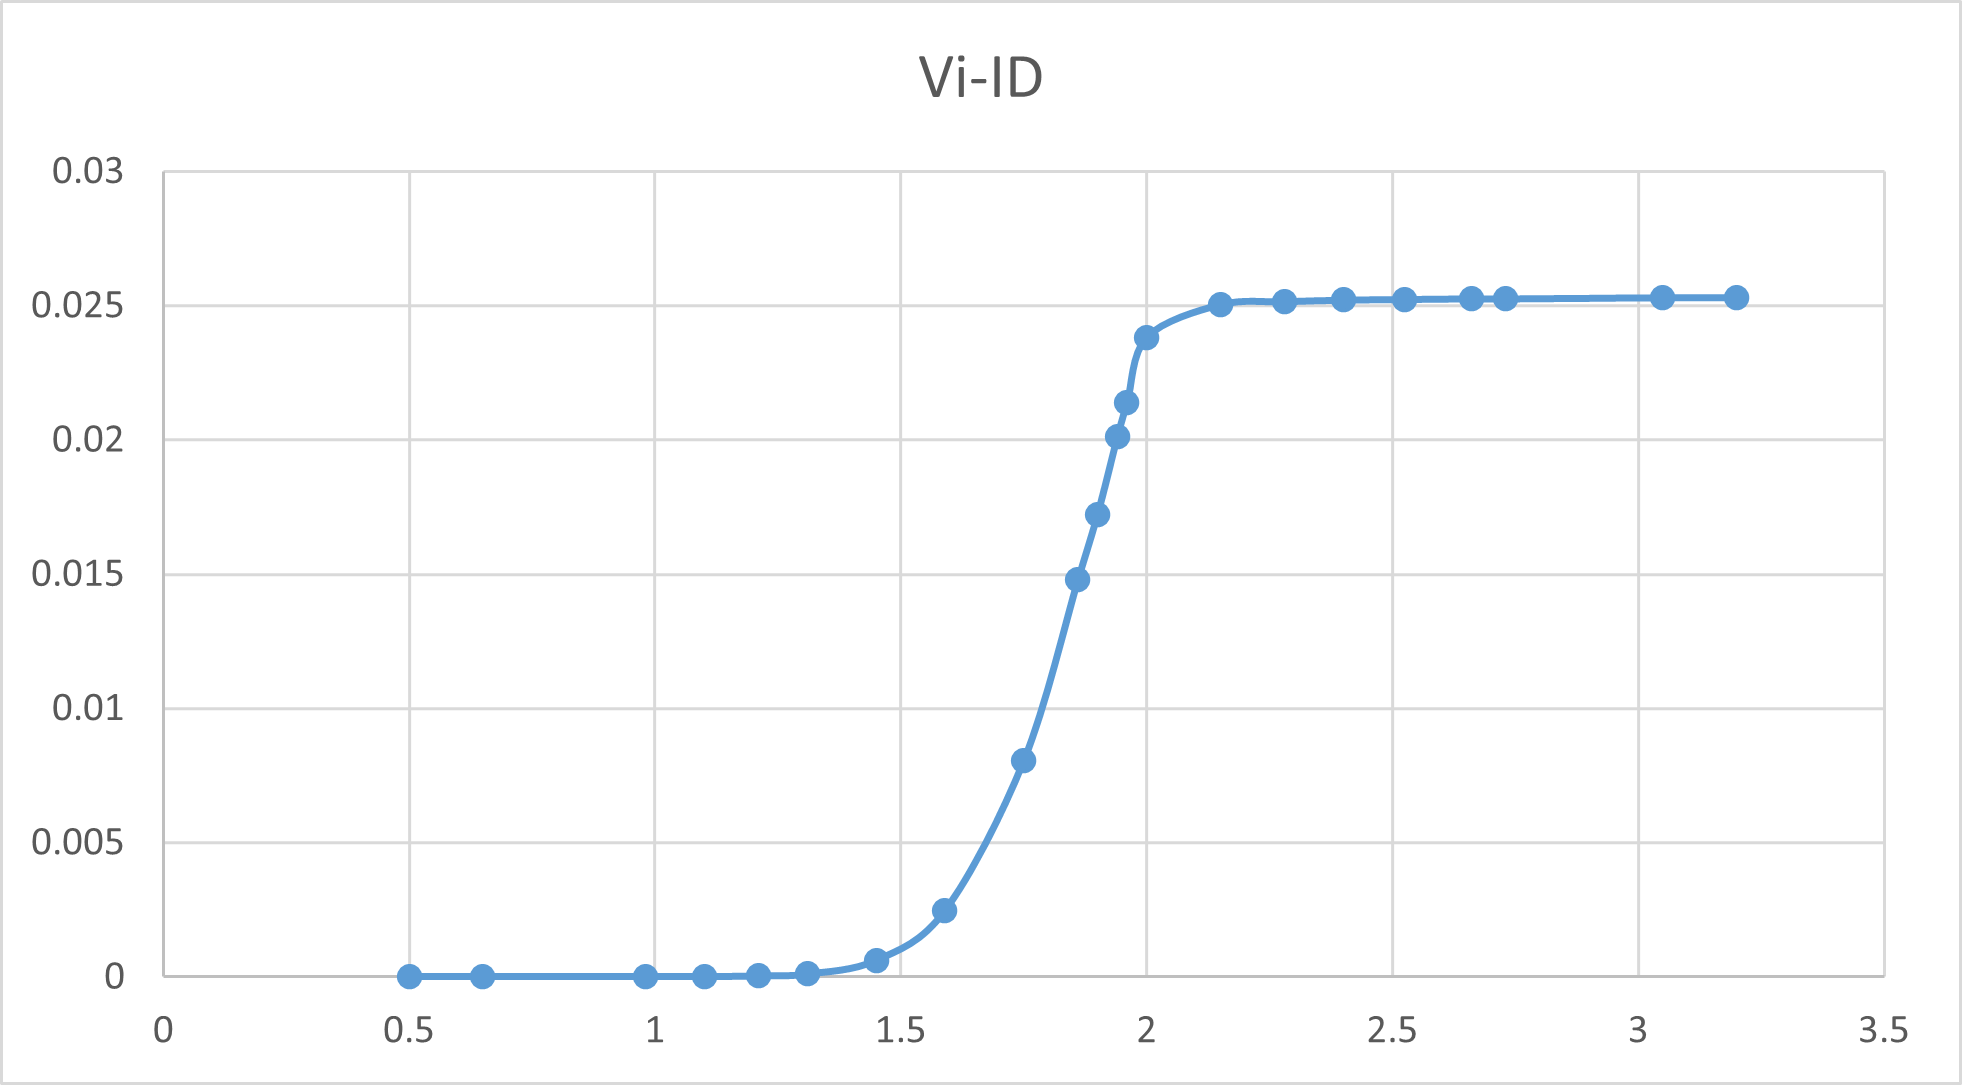
\includegraphics[width=0.5\linewidth]{Experiment_08/Images/L8_DCF2.png}
        \caption{Relationship between $V_{GS}$ and $I_D$}
        \label{l8dctf2}
    \end{figure}
    \FloatBarrier
    Relationship between $V_{GS}$ and $\sqrt{I_D}$:\\
    \begin{figure}[H]
        \centering
        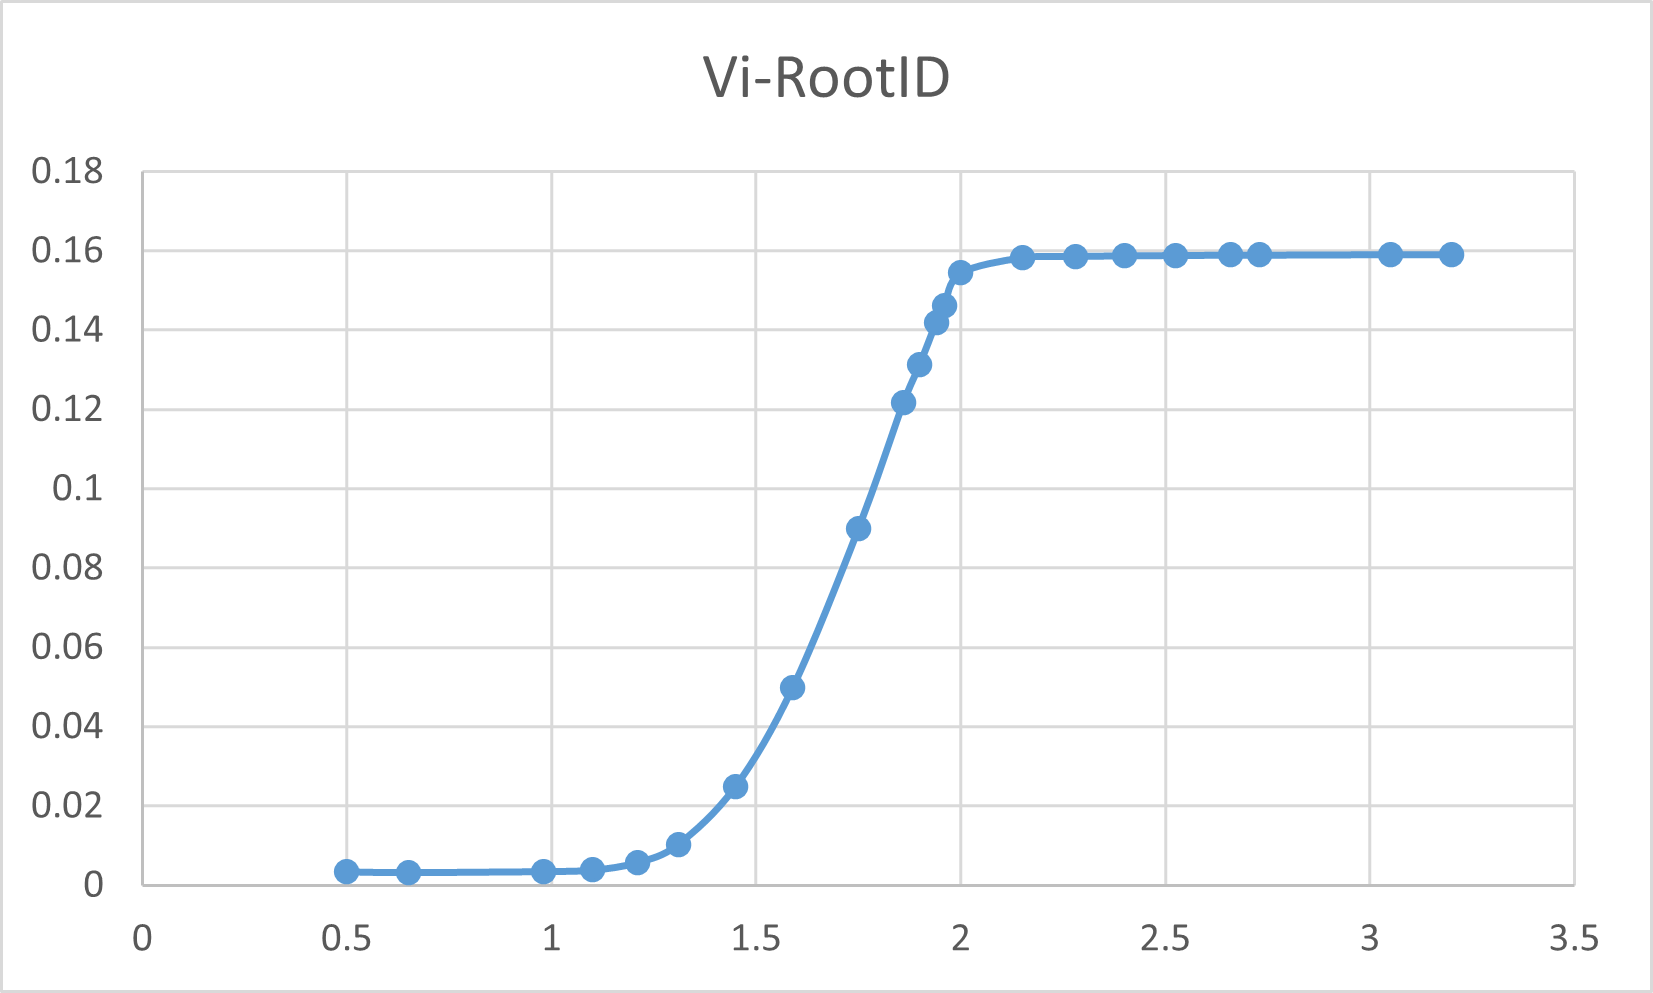
\includegraphics[width=0.65\linewidth]{Experiment_08/Images/L8_DCF3.png}
        \caption{Relationship between $V_{GS}$ and $\sqrt{I_D}$}
        \label{L8dctf3}
    \end{figure}
\FloatBarrier
    From these figures we can conclude that $V_{TH}$ = 1.2V and $K_n$ =  0.067 $A/V^2$.

    \subsubsection{Part II}
    The data we recorded for the MOSEFT circuit is shown in the following table:
    \begin{table}[H]
        \centering
% Table generated by Excel2LaTeX from sheet 'Sheet1'
\begin{tabular}{l|rrrrrrrrrrrrrrrrrr}
    \midrule
    $Vi=1.6 $  &       &       &       &       &       &       &       &       &       &       &       &       &       &       &       &       &       &  \\
    \midrule
    $V+     $ & 0.17  & 0.34  & 0.42  & 0.78  & 1.07  & 1.56  & 2.22  & 2.67  & 2.9   & 3.3   & 4.08  & 4.95  & 5.36  & 5.64  & 5.96  & 6.44  &       &  \\
    $VDS    $ & 0.012 & 0.032 & 0.042 & 0.137 & 0.299 & 0.697 & 1.31  & 1.74  & 1.93  & 2.31  & 3.07  & 3.89  & 4.28  & 4.56  & 4.86  & 5.33  &       &  \\
    $VR_D   $ & 0.156 & 0.305 & 0.36  & 0.64  & 0.76  & 0.831 & 0.873 & 0.895 & 0.905 & 0.92  & 0.95  & 0.982 & 0.999 & 1.01  & 1.022 & 1.04  &       &  \\
\midrule \midrule
    $Vi=1.7 $  &       &       &       &       &       &       &       &       &       &       &       &       &       &       &       &       &       &  \\
    $V+     $ & 0.01  & 0.3   & 0.66  & 1.11  & 1.62  & 2.31  & 2.94  & 3.5   & 3.97  & 4.44  & 5.04  & 5.59  & 6.16  & 6.76  & 7.26  & 7.6   & 7.78  &  \\
    $VDS    $ & 0     & 0.012 & 0.035 & 0.072 & 0.14  & 0.4   & 0.86  & 1.36  & 1.77  & 2.18  & 2.72  & 3.2   & 3.72  & 4.28  & 4.7   & 5.05  & 5.2   &  \\
    $VR_D   $ & 0.01  & 0.284 & 0.621 & 1.04  & 1.48  & 1.91  & 2.05  & 2.13  & 2.16  & 2.2   & 2.25  & 2.31  & 2.35  & 2.4   & 2.45  & 2.47  & 2.49  &  \\
    \midrule
    \midrule
    $Vi=1.8 $  &       &       &       &       &       &       &       &       &       &       &       &       &       &       &       &       &       &  \\
    $V+     $ & 0.3   & 0.52  & 0.74  & 1.05  & 1.31  & 1.88  & 2.12  & 2.47  & 2.99  & 3.59  & 4.19  & 4.89  & 5.48  & 6.59  & 7.49  & 8.13  & 9.25  & 9.82 \\
    $VDS    $ & 0.007 & 0.015 & 0.023 & 0.035 & 0.046 & 0.075 & 0.089 & 0.112 & 0.157 & 0.244 & 0.43  & 0.84  & 1.3   & 2.2   & 2.95  & 3.5   & 4.43  & 4.9 \\
    $VR_D   $ & 0.291 & 0.5   & 0.71  & 1.01  & 1.26  & 1.8   & 2.03  & 2.35  & 2.82  & 3.34  & 3.75  & 4.02  & 4.15  & 4.33  & 4.47  & 4.58  & 4.73  & 4.86 \\
    \midrule \midrule
        $Vi=1.9 $  &       &       &       &       &       &       &       &       &       &       &       &       &       &       &       &       &       &  \\
        \midrule
    $V+     $ & 0.4   & 1.13  & 2.3   & 3.17  & 4.38  & 5.29  & 6.68  & 7.3   & 7.76  & 8.19  & 8.49  & 9.72  & 10.26 & 11.19 & 12.23 & 12.82 & 13.26 & 13.67 \\
    $VDS    $ & 0.008 & 0.026 & 0.06  & 0.09  & 0.143 & 0.2   & 0.37  & 0.5   & 0.77  & 1.02  & 1.43  & 2.05  & 2.44  & 3.2   & 3.9   & 4.33  & 4.6   & 4.93 \\
    $VR_D   $ & 0.39  & 1.1   & 2.23  & 3.07  & 4.24  & 5.09  & 6.3   & 6.75  & 6.97  & 7.14  & 7.33  & 7.6   & 7.75  & 7.94  & 8.24  & 8.42  & 8.58  & 8.66 \\
    \midrule
    \end{tabular}%
    
        \caption{The transfer characteristics of MOSEFT}
        \label{tab:}
    \end{table}

    Using this table, we can draw the relationship between $V_{DS}$ and $V_{R_D}$ for different values of $V_i$.
    
\subsection{Experiment Conclusion}
    \subsubsection{Conclusion}
\section{A Common-Source Amplifier}

\subsection{Experiment Design}
    \subsubsection{Background}


    \subsubsection{Propose}
    \begin{itemize}
        \item 2N7000 MOSEFT
        \item Resistors
        \item Breadboard
        \item Oscilloscope
        \item Function Generator
        \item DC Power Supply
    \end{itemize}

\subsection{Experiment Design}
    \subsubsection{Materials}
        In this experiment, we will use the following components:
        \begin{itemize}
            \item To measure the quiescent-point of a common-source amplifier
            \item To evaluate the small-signal amplification function of a common-source amplifier
        \end{itemize}

    \subsubsection{Circuit Diagram}
        The following circuit diagrams 
        \begin{figure}[H]
            \centering
                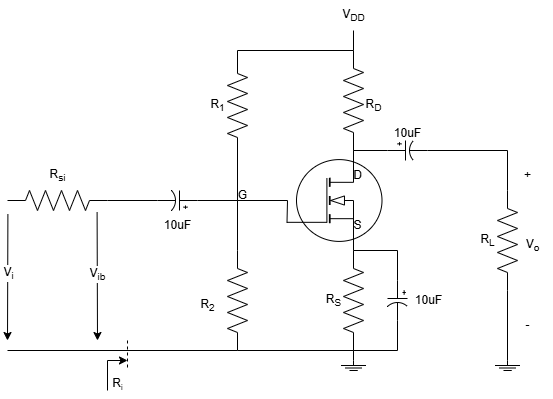
\includegraphics[width=1\linewidth]{Experiment_09/Circuit/Lab9.drawio.png}
                \caption{Common-Source Amplifier Circuit}
                \label{cir:9}
        \end{figure}

    \subsubsection{Theoretical Analysis}
        \begin{enumerate}[a]
            \item \textbf{DC Analysis}\par
                \begin{figure}[H]
                    \centering
                        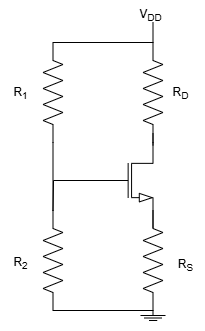
\includegraphics[width=0.3\linewidth]{Experiment_09/Circuit/L9DC.drawio.png}
                        \caption{DC equvlent Circuit}
                        \label{cir:9DC}
                \end{figure}
            \item \textbf{AC Analysis}\par
                \begin{figure}[H]
                    \centering
                        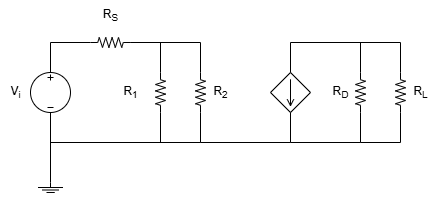
\includegraphics[width=0.3\linewidth]{Experiment_09/Circuit/L9AC.drawio.png}
                        \caption{AC equvlent Circuit}
                        \label{cir:9AC}
                \end{figure}
        \end{enumerate}

\subsection{Experiment record}
    \subsubsection{Voltage gain}
    We recorded the following data to calculate voltage gain of the common-source amplifier:
    \begin{table}[h]
        \centering
        \begin{tabular}{l|rrrr}
            Vib   & 0.0646 & 0.052 & 0.039 & 0.025 \\
            Vo    & 0.51  & 0.413 & 0.309 & 0.205 \\
            \midrule
            A     & 7.894737 & 7.942308 & 7.923077 & 8.2 \\
            \end{tabular}%
        \caption{Voltage gain}
    \end{table}
    The voltage gain is calculated with the formula: $\frac{V_O}{V_I}$

    \subsubsection{Input impedance}
    \begin{table}[h]
        \centering
    \begin{tabular}{lr}
        Vib   & 0.066 \\
        Vi    & 0.072 \\
        \end{tabular}%
        \caption{Input impedance}
    \end{table}
    And the input impedance is calculated as:
        
    \subsubsection{Output impedance}
    To calculate the output impedance, we recorded the following data:
    \begin{table}[h]
        \centering
    \begin{tabular}{lcc}
        AC OR & RL = 300k & RL = 1k \\
        Vi    & 0.073 & 0.0.73 \\
        Vo    & 0.522 & 0.436 \\
        \end{tabular}%
        \caption{Output impedance}
    \end{table}

\subsection{Experiment Conclusion}
    \subsubsection{Conclusion}
    This experiment presents us the common-source MOSFET amplifier. The experiment reinforces my understanding of the MOSFET circuit.\par
\section{Mathematical Circuits Using the Op. Amp.: part I}

\subsection{Experiment Design}
    \subsubsection{Background}
    The operational amplifier can be used to consruct circuite to implement amplification and mathematical operations. In this experiment, we will implement six function using the combination of Op.Amp. and other components.\par

    \subsubsection{Propose}
    \begin{itemize}
        \item To verify Op.Amp. circuits for basic amplification operations
        \item To verify Op.Amp. circuits for addition/substraction
    \end{itemize}

\subsection{Experiment Design}
    \subsubsection{Materials}
        In this experiment, we will use the following components:
        \begin{itemize}
            \item Capacitors
            \item 1N4148 Diode
            \item LM741\_1 Op.Amp.
            \item Resistors
            \item Breadboard
            \item DC power supply
            \item Digital Multi-Meter
            \item Function Generator
        \end{itemize}

    \subsubsection{Circuit Diagram}
        The following circuit diagrams shows the Op.Amp. circuits for differentiation, integration, logarithm and exponential operations.
        \begin{figure}[H]
            \centering
            \begin{subfigure}{0.4\textwidth}
                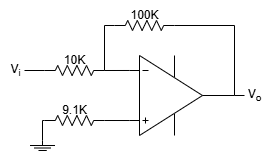
\includegraphics[width=1\linewidth]{Experiment_10/Circuit/Lab10a.drawio.png}
                \caption{Inverting Amplifier}
                \label{cir:InvAmp}
            \end{subfigure}
            \begin{subfigure}{0.4\textwidth}
                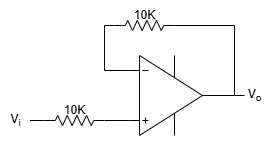
\includegraphics[width=1\linewidth]{Experiment_10/Circuit/Lab10b.drawio.png}
                \caption{Voltage Follower}
                \label{cir:VolFAmp}
            \end{subfigure}

            \begin{subfigure}{0.4\textwidth}
                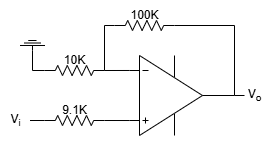
\includegraphics[width=1\linewidth]{Experiment_10/Circuit/Lab10c.drawio.png}
                \caption{Non-Inverting Amplifier}
                \label{cir:NInvAmp}
            \end{subfigure}
            \begin{subfigure}{0.4\textwidth}
                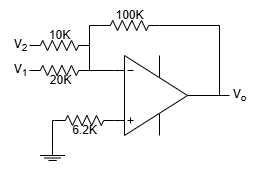
\includegraphics[width=1\linewidth]{Experiment_10/Circuit/Lab10d.drawio.png}
                \caption{Summing Amplifier}
                \label{cir:SumAmp}
            \end{subfigure}

            \begin{subfigure}{0.4\textwidth}
                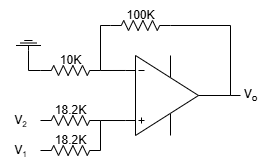
\includegraphics[width=1\linewidth]{Experiment_10/Circuit/Lab10e.drawio.png}
                \caption{Non-Inverting Summing Amplifier}
                \label{cir:NSumAmp}
            \end{subfigure}
            \begin{subfigure}{0.4\textwidth}
                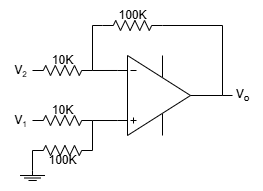
\includegraphics[width=1\linewidth]{Experiment_10/Circuit/Lab10f.drawio.png}
                \caption{Difference Amplifier}
                \label{cir:DiffAmp}
            \end{subfigure}

            \caption{Circuit Diagrams for Op.Amp. Circuits}
        \end{figure}

    \subsubsection{Theoretical Analysis}
        \begin{enumerate}[a]
            \item \textbf{Inverting Amplifier}\newline
                From the figure \ref{cir:InvAmp}, 
                we reconize this is an inverting amplifier. The output voltage can be calculated by the following equation:
                \begin{equation}
                    \frac{V_i}{R_i} = \frac{V_o}{R_{feedback}}
                \end{equation}
                Where in our circuit, the $R_i = 10k \Omega$ and $R_{feedback} = 100k \Omega$ . So plugging in the values, we get:
                \begin{equation}
                    V_o = -10V_i
                    \label{eq:InvAmp_output}
                \end{equation}

            \item \textbf{Voltage Follower}\newline
                From the figure \ref{cir:VolFAmp}, we can see that the output voltage is the same as the input voltage. So the output voltage can be calculated by the following equation:
                \begin{equation}
                    V_o = V_i
                    \label{eq:VolF_output}
                \end{equation}

                \item \textbf{Non-Inverting Amplifier}\newline
                From the figure \ref{cir:NInvAmp}, we can see that the output voltage can be calculated by the following equation:
                \begin{equation}
                    \frac{V_i}{R_i} = \frac{V_i-V_o}{R_{feedback}}
                \end{equation}
                Where in our circuit, the $R_i = 10k \Omega$ and $R_{feedback} = 100k \Omega$ . So plugging in the values, we get:
                \begin{equation}
                    V_o = 11V_i
                    \label{eq:NInvAmp_output}
                \end{equation}

            \item \textbf{Summing Amplifier}\newline
                From the figure \ref{cir:SumAmp}, we can see that the output voltage can be calculated by the following equation:
                \begin{equation}
                    \frac{V_{i1}}{R_{i1}} + \frac{V_{i2}}{R_{i2}} = \frac{V_o}{R_{feedback}}
                \end{equation}
                Where in our circuit, the $R_{i1} = 10k \Omega$, $R_{i2} = 20k \Omega$ and $R_{feedback} = 100k \Omega$ . So plugging in the values, we get:
                \begin{equation}
                    V_o = -10V_2 - 5V_1
                    \label{eq:SumAmp_output}
                \end{equation}

            \item \textbf{Non-Inverting Summing Amplifier}\newline
                From the figure \ref{cir:NSumAmp}, we can see that the output voltage can be calculated by the following equation:
                \begin{equation}
                    V_o = (10+1)V_X
                \end{equation}
                Where $V_X$ is given by the following equation:
                \begin{equation}
                    V_X = \frac{V_{i1}}{R_{i1}} + \frac{V_{i2}}{R_{i2}}
                \end{equation}
                In our circuit, the $R_{i1} = 18.2k \Omega$, $R_{i2} = 18.2k \Omega$ and $R_{feedback} = 100k \Omega$ . So plugging in the values, we get:
                \begin{equation}
                    V_o = \frac{11}{2}(V_2+V_1)
                    \label{eq:NSumAmp_output}
                \end{equation}

            \item \textbf{Difference Amplifier}\newline
                From the figure \ref{cir:DiffAmp}, we can see that the output voltage can be calculated by the following equation:
                \begin{equation}
                    \begin {aligned}
                    \frac{0-V_X}{R_{feedback}} + \frac{V_1-V_X}{R_1} = 0
                    \frac{V_2-V_X}{R_{2}} = 0 + \frac{V_X-V_O}{R_{feedback}} = 0
                    \end {aligned}
                \end{equation}
                Where in our experiment, the $R_1 = 10k \Omega$ and $R_{feedback} = 100k \Omega$ . So plugging in the values, we can slove for $V_O$:
                \begin{equation}
                    V_O = 10V_1 - 10V_2
                    \label{eq:DiffAmp_output}
                \end{equation}
        \end{enumerate}

\subsection{Experiment record}
    \subsubsection{The Inverting Amplifier}
    \begin{enumerate}[I]
        \item \textbf{Data Recorded}\newline
            The recorded data for the integration operation circuit is shown in the following table:
            \begin{table}[H]
                \centering
                \begin{tabular}{l|rrrrrrrr}
                \toprule
                $V_i$ & 0.10  & 0.30  & 0.50  & 0.70  & 0.90  & 1.10  & 1.30  & 1.50 \\
                \midrule
                $V_o$ (Mea) & -1.00 & -3.05 & -5.09 & -7.11 & -9.16 & -11.15 & -11.36 & -11.36 \\
                \midrule
                $V_o$ (Theo) & -1.00 & -3.00 & -5.00 & -7.00 & -9.00 & -11.00 & -13.00 & -15.00 \\
                Error & 0.00\% & 0.03\% & 0.03\% & 0.02\% & 0.03\% & 0.02\% & 1.59\% & 5.89\% \\
                \bottomrule
                \end{tabular}%
                \caption{Recorded Data for the Inverting Amplifier}
                \label{tab:InvAmp}
            \end{table}
        \item \textbf{Data Analysis}\newline
            The theoretical output voltage for the inverting amplifier is calculated by the equation \ref{eq:InvAmp_output}. And the square error between the measured and theoretical output voltage is calculated and shown in the table \ref{tab:InvAmp}.\par
            
            Reading the table, we can see that the error between the measured and theoretical output voltage is small, so our circuit is working as expected. And we can notice the ouput voltage is bound to the maximum value of 11.36V, which is the value of the reference voltage.\par
    \end{enumerate}
    
    \subsubsection{The Voltage Follower}
    \begin{enumerate}[I]
        \item \textbf{Data Recorded}\newline
            The recorded data for the integration operation circuit is shown in the following table:
            \begin{table}[H]
                \centering
                \begin{tabular}{l|rrrrrrrr}
                    \toprule
                    $V_i$ & 0.100 & 0.300 & 0.500 & 0.700 & 0.900 & 1.100 & 1.300 & 1.500 \\
                    \midrule
                    $V_o$ (Mea) & 0.091 & 0.299 & 0.499 & 0.695 & 0.896 & 1.096 & 1.296 & 1.498 \\
                    \midrule
                    $V_o$ (Theo) & 0.100 & 0.300 & 0.500 & 0.700 & 0.900 & 1.100 & 1.300 & 1.500 \\
                    Error & 0.81\% & 0.00\% & 0.00\% & 0.01\% & 0.00\% & 0.00\% & 0.00\% & 0.00\% \\
                    \bottomrule
                    \end{tabular}%
                    \caption{Recorded Data for the Voltage Follower}
                    \label{tab:VolFAmp}
            \end{table}
        \item \textbf{Data Analysis}\newline\
            The theoretical output voltage for the voltage follower is calculated by the equation \ref{eq:VolF_output}. And the square error between the measured and theoretical output voltage is calculated and shown in the table \ref{tab:VolFAmp}.\par

            From the table, we can notice the error is very small. This shows our circuit is working as expected. And because the output voltage is below the reference voltage, there were no saturation as was in the last experiment.\par
    \end{enumerate}

    \subsubsection{The Non-Inverting Amplifier}
    \begin{enumerate}[I]
        \item \textbf{Data Recorded}\newline
            The recorded data for the integration operation circuit is shown in the following table:
            \begin{table}[H]
                \centering
                \begin{tabular}{l|rrrrrrrr}
                    \toprule
                    $V_i$ & 0.10  & 0.30  & 0.50  & 0.70  & 0.90  & 1.10  & 1.30  & 1.50 \\
                    \midrule
                    $V_o$ (Mea) & 1.09  & 3.32  & 5.51  & 7.76  & 10.02 & 10.64 & 10.64 & 10.64 \\
                    \midrule
                    $V_o$ (Theo) & 1.10  & 3.30  & 5.50  & 7.70  & 9.90  & 12.10 & 14.30 & 16.50 \\
                    Error & 0.01\% & 0.00\% & 0.00\% & 0.01\% & 0.01\% & 1.46\% & 6.55\% & 12.61\% \\
                    \bottomrule
                    \end{tabular}%
                    \caption{Recorded Data for the Non-Inverting Amplifier}
                    \label{tab:NInvAmp}
            \end{table}
        \item \textbf{Data Analysis}\newline
            The theoretical output voltage for the non-inverting amplifier is calculated by the equation \ref{eq:NInvAmp_output}. And the square error between the measured and theoretical output voltage is calculated and shown in the table \ref{tab:NInvAmp}.\par

            From the table, we can notice the error is small. This shows our circuit is working as expected. And we can notice the ouput voltage is bound to the maximum value of 10.64V, which is about the value of the reference voltage 11V.\par
    \end{enumerate}

    \subsubsection{The Summing Amplifier}
    \begin{enumerate}[I]
        \item \textbf{Data Recorded}\newline
            The recorded data for the integration operation circuit is shown in the following table:
            \begin{table}[H]
                \centering
                \begin{tabular}{l|rrrr}
                    \toprule
                    $V_1$ & 0.10  & 0.50  & 0.10  & 1.00 \\
                    $V_2$ & 0.20  & 0.10  & 0.50  & 0.40 \\
                    \midrule
                    $V_o$ (Mea) & -2.05 & -3.52 & -5.58 & -11.36 \\
                    \midrule
                    $V_o$ (Theo) & -2.50 & -3.50 & -5.50 & -9.00 \\
                    Error & 3.20\% & 0.00\% & 0.02\% & 6.89\% \\
                    \bottomrule
                    \end{tabular}
                \caption{Recorded Data for the Summing Amplifier}
                \label{tab:SumAmp}
            \end{table}
        \item \textbf{Data Analysis}\newline
            The theoretical output voltage for the summing amplifier is calculated by the equation \ref{eq:SumAmp_output}. And the square error between the measured and theoretical output voltage is calculated and shown in the table \ref{tab:SumAmp}.\par

            From the table, we can notice the error is small. This shows our circuit is working as expected.\par
    \end{enumerate}

    \subsubsection{The Non-Inverting Summing Amplifier}
    \begin{enumerate}[I]
        \item \textbf{Data Recorded}\newline
            The recorded data for the integration operation circuit is shown in the following table:
            \begin{table}[H]
                \centering
                \begin{tabular}{|l|rrrr|}
                    \toprule
                    $V_1$ & 0.100 & 0.500 & 0.800 & 1.000 \\
                    $V_2$ & 0.200 & 0.300 & 0.500 & 1.000 \\
                    \midrule
                    $V_o$ (Mea) & 1.640 & 4.439 & 7.205 & 10.638 \\
                    \midrule
                    $V_o$ (Theo) & 1.650 & 4.400 & 7.150 & 11.000 \\
                    Error & 0.00\% & 0.01\% & 0.01\% & 0.11\% \\
                    \bottomrule
                    \end{tabular}%
            \caption{Recorded Data for the Non-Inverting Summing Amplifier}
            \label{tab:NSumAmp}                    
            \end{table}
        \item \textbf{Data Analysis}\newline
            The theoretical output voltage for the non-inverting summing amplifier is calculated by the equation \ref{eq:NSumAmp_output}. And the square error between the measured and theoretical output voltage is calculated and shown in the table \ref{tab:NSumAmp}.\par

            From the table, we can notice the error is small. This shows our circuit is working as expected. Note at the last data, the output is limited to 10.638V, which's around the voltage of the reference voltage 11V.\par
    \end{enumerate}

    \subsubsection{The Difference Amplifier}
    \begin{enumerate}[I]
        \item \textbf{Data Recorded}\newline
            The recorded data for the integration operation circuit is shown in the following table:
            \begin{table}[H]
                \centering
                \begin{tabular}{|l|rrr|}
                    \toprule
                    $V_1$ & 0.10  & 0.50  & 1.00 \\
                    $V_2$ & 0.40  & 0.10  & 0.40 \\
                    \midrule
                    $V_o$ (Mea) & -3.18 & 4.16  & 6.17 \\
                    \midrule
                    $V_o$ (Theo) & -3.00 & 4.00  & 6.00 \\
                    Error & 0.36\% & 0.15\% & 0.08\% \\
                    \bottomrule
                    \end{tabular}%
                \caption{Recorded Data for the Difference Amplifier}
                \label{tab:DiffAmp}
            \end{table}

        \item \textbf{Data Analysis}\newline
            The theoretical output voltage for the difference amplifier is calculated by the equation \ref{eq:DiffAmp_output}. And the square error between the measured and theoretical output voltage is calculated and shown in the table \ref{tab:DiffAmp}.\par

            From the table, we can notice the error is small. This shows our circuit is working as expected.\par
    \end{enumerate}


\subsection{Experiment Conclusion}
    \subsubsection{Conclusion}
        In this experiment, we have implemented six mathematical operations using the Op.Amp. circuits. The output voltage of the circuits were calculated and compared with the theoretical output voltage. The error between the measured and theoretical output voltage was calculated and analyzed. From the analysis, we can conclude that the circuits are working as expected.\par
\section{Mathematical Circuits Using the Op. Amp.: part II}

\subsection{Experiment Design}
    \subsubsection{Background}
    Besides basic amplification and basic algebraic operations, the operational amplifier can also be used to perform mathematical operations like differnciation, intergration, logarithm etc. And in this experiment, we will implement four mathematical operations using the operational amplifier.

    \subsubsection{Propose}
    \begin{itemize}
        \item To verify the Op.Amp. circuit for differentiation operation.
        \item To verify the Op.Amp. circuit for integration operation.
        \item To verify the Op.Amp. circuit for logarithm operation.
        \item To verify the Op.Amp. circuit for exponential operation.
    \end{itemize}

\subsection{Experiment Design}
    \subsubsection{Materials}
        In this experiment, we will use the following components:
        \begin{itemize}
            \item Capacitors
            \item 1N4148 Diode
            \item LM741\_1 Op.Amp.
            \item Resistors
            \item Breadboard
            \item DC power supply
            \item Digital Multi-Meter
            \item Oscilloscope
            \item Function Generator
        \end{itemize}

    \subsubsection{Circuit Diagram}
        The following circuit diagrams shows the Op.Amp. circuits for differentiation, integration, logarithm and exponential operations.
        \begin{figure}[H]
            \centering
            \begin{subfigure}{0.4\textwidth}
                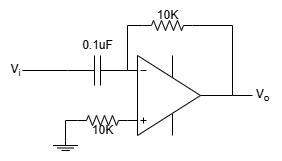
\includegraphics[width=1\linewidth]{Experiment_11/Circuit/Lab11a.drawio.png}
                \caption{Circuit of Differentiation}
                \label{cir:diff}
            \end{subfigure}
            \begin{subfigure}{0.4\textwidth}
                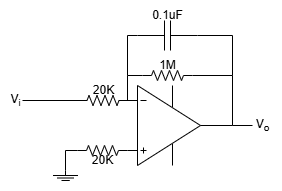
\includegraphics[width=1\linewidth]{Experiment_11/Circuit/Lab11b.drawio.png}
                \caption{Circuit of Integration}
                \label{cir:int}
            \end{subfigure}

            \begin{subfigure}{0.4\textwidth}
                \includegraphics[width=1\linewidth]{Experiment_11/Circuit/Lab11c.drawio.png}
                \caption{Circuit of Logarithm}
                \label{cir:log}
            \end{subfigure}
            \begin{subfigure}{0.4\textwidth}
                \includegraphics[width=1\linewidth]{Experiment_11/Circuit/Lab11d.drawio.png}
                \caption{Circuit of Exponential}
                \label{cir:exp}
            \end{subfigure}
            \caption{Op.Amp. Circuits for Mathematical Operations}
        \end{figure}

    \subsubsection{Theoretical Analysis}
        \begin{enumerate}
            \item \textbf{Differentiation Operation}\newline
                From the figure \ref{cir:diff}, 
                we can see the feedback is through a resistor, and the input voltage is connct to the negetive terminal of the Op.Amp. through a capacitor. 
                So we conclude that this circuit is a differentiator circuit. The output voltage of the circuit is given by:
                \begin{equation}
                    V_{out} = -RC\frac{dV_{in}}{dt}
                \end{equation}
                Where in our circuit, the $R = 1M \Omega$ and $C = 0.1\mu F$.
                \newline

            \item \textbf{Integration Operation}\newline
                From the figure \ref{cir:int}, 
                we can see the feedback is through a parallel conncetion of a resistor and a capacitor, and the input voltage is connct to the negetive terminal of the Op.Amp. through a resistor.
                So we can see it's an integrator circuit. The output voltage of the circuit is given by:
                \begin{equation}
                    V_{out} = -\frac{1}{RC}\int V_{in}dt
                \end{equation}
                Where in our circuit, the $R = 10k \Omega$ and $C = 0.1\mu F$.
                \newline

            \item \textbf{Logarithm Operation}\newline
                From the figure \ref{cir:log}, one may notice the feedback is through a dioide, and the input voltage is connct to the negetive terminal of the Op.Amp. through a resistor.
                So we can see this is logarithm circuit. The output voltage of the circuit is given by:
                \begin{equation}
                    V_{out} = -\frac{R_2}{R_1}ln\left(\frac{V_{in}}{V_{ref}}\right)
                \end{equation}
                Where in our circuit, the $V_{ref}$ is the amplitude of the reference voltage, and $R_1 = R_2 = 100k \Omega$.
                \newline
            \item \textbf{Exponential Operation}\newline
                From the figure \ref{cir:exp}, we notice the feedback is through a resistor, and the input voltage is connct to the negetive terminal of the Op.Amp. through a dioide.
                So we know this circuit is an exponential circuit. The output voltage of the circuit is given by:
                \begin{equation}
                    V_{out} = V_{ref}e^{V_{in}}
                    \label{eq:exp}
                \end{equation}
                Where in our circuit, the $V_{ref}$ is the reference voltage.
        \end{enumerate}

\subsection{Experiment record}
    \subsubsection{The intergration operation circuit}
    \begin{enumerate}[I]

        \item \textbf{Data Recorded}\newline
            The recorded data for the differentiation operation circuit is shown in the table \ref{tab:diff}.
            % Table generated by Excel2LaTeX from sheet 'Sheet1'
            \begin{table}[H]
                \centering
                \begin{tabular}{l|rrrrr}
                    Frequency ($Hz$) & 200.00  & 400.00  & 600.00  & 800.00  & 1000.00  \\
                    \midrule
                    Ampititude ($mV$) & 1800  & 2900  & 4200  & 5450  & 6650  \\
                    Phase ($^\circ$) & 94.56  & 94.40  & 91.53  & 96.43  & 97.49  \\
                \end{tabular}%
                \caption{Data Recorded for Differentiation Operation}
                \label{tab:diff}
            \end{table}
            In addition, here is the plot of the output voltage versus the input voltage for the circuit when connect to a square wave signal.
            \begin{figure}[H]
                \centering
                \includegraphics[width=0.6\linewidth]{Experiment_11/Images/cir1_squar.jpg}
                \caption{Output waveform with square wave signal input}
                \label{wave:diff}
            \end{figure}

        \item \textbf{Data Analysis}\newline
            From the output table \ref{tab:diff}, we can see as the Frequency of the input signal increase, the amplitude and the phase difference between input and output increase.\par 
            
            This is beacuse as the frequency increase, the rate of change of the input signal also increase, thus we have a higher amplitude as output, as the output is giving by 
                \begin{equation*}
                    V_{out} = -RC\frac{dV_{in}}{dt}
                \end{equation*}
            \par

            And the phase difference increases because circuit is not ideal, and have a higher phase shifts at higher frequencies.\par

            Finally, with respect to the output wave form in figure \ref{wave:diff}. This is because the rate of change of the square wave is approximately infinite at its edges, so the output is a spike at the edges of the square wave.
    \end{enumerate}

    \subsubsection{The intergration operation circuit}
    \begin{enumerate}
        \item \textbf{Data Recorded}\newline
            The recorded data for the integration operation circuit is shown in the table \ref{tab:int}.

            \begin{table}[H]
            % Table generated by Excel2LaTeX from sheet 'Sheet1'
                \centering
                \begin{tabular}{l|rrrr}
                Frequency $Hz$ & 50.00  & 100.00  & 150.00  & 200.00  \\
                \midrule
                Ampititude $V$ & 1.850  & 0.935  & 0.615  & 0.470  \\
                Phase $^\circ$ & -104.16 & -93.47 & -89.7 & -89.83 \\
                \end{tabular}%
                \caption{Data Recorded for Integration Operation}
                \label{tab:int}
            \end{table}

            In addition, this is the plot of the output voltage versus the input voltage for the circuit when connect to a square wave signal.
            \begin{figure}[H]
                \centering
                \includegraphics[width=0.6\linewidth]{Experiment_11/Images/cir2_squar.jpg}
                \caption{Output waveform with square wave signal input}
                \label{wave:int}
            \end{figure}

            From the table \ref{tab:int}, we can see as the Frequency of the input signal increase, the amplitude of output decrease. And the phase difference is not in ideal 90$^\circ$, but approching to 90$^\circ$ as frequency increase.\par
        \item \textbf{Data Analysis}\newline
            The amplitude of the output decreases because at higher frequencies, the input signal oscillates faster, and its area (integral) over each cycle becomes smaller. So the output voltage have a smaller amplitude.\par

            The phase difference is negetive because the output is lagging behind the input signal for $\frac{\pi}{2}$. And when the frequency is low, the capacitor reduce the speed of responds, and causing a non perfect phase difference. However, as the frequency increase, the capacitor behave more like a ideal conducter, and the phase difference approching to our expected value.\par

            Finally, with respect to the output wave form in figure \ref{wave:int}. This is because the output is the integral of the input signal, so the output is a triangle wave.
    \end{enumerate}

    \subsubsection{The logarithm operation circuit}
    \begin{enumerate}
        \item \textbf{Data Recorded}\newline
            When the input signal is a triangular wave, the output signal and the input signal is record by the Oscilloscope, and the plot is shown in the figure \ref{wave:log}.
            \begin{figure}[H]
                \centering
                \includegraphics[width=0.6\linewidth]{Experiment_11/Images/cir3_tri.jpg}
                \caption{Output waveform of log circuit with triangular wave signal input}
                \label{wave:log}
            \end{figure}
        \item \textbf{Data Analysis}\newline
            From the ouput wave form in figure \ref{wave:log}, we can see the the output signal is always at zero, around the positive peak of the input signal, the output signal drop to negetive very quickly, and recover to zero quickly when the input signal drop after its peak.\par

            This is because the logarithmic function changes very slowly except near rapid transitions so the output remains close to zero during most of the input. And therefore, at the peak of the input signal, the signal change rapidly, so the output will quickly goes to a extream value quickly. Howver, when the signal approch to the negetive edge, the diode at the feedback loop block the output signal from change to a positive peak, so the ouput looks like what we saw.\par
    \end{enumerate}

    \subsubsection{The exponential operation circuit}
    \begin{enumerate}
        \item \textbf{Data Recorded}\newline
            When the input signal is a triangular wave, the output signal and the input signal is record by the Oscilloscope, and the plot is shown in the figure \ref{wave:exp}.
            \begin{figure}[H]
                \centering
                \includegraphics[width=0.6\linewidth]{Experiment_11/Images/cir4_tri.jpg}
                \caption{Output waveform of exponential circuit with triangular wave signal input}
                \label{wave:exp}
            \end{figure}
        \item \textbf{Data Analysis}\newline
            From the output wave form in figure \ref{wave:exp}, we can see at the increase ramp, the output voltage drop in the exponential curve, and at the decrease ramp, the output voltage rise in the exponential curve.\par

            Beacuse the characteristic of the circuit, the output signal behave inversely to the input signal. And due to the exponential nature of the circuit, the output signal is exponential to the input signal as the output signal euqation eq.\ref{eq:exp} shows.\par
    \end{enumerate}

\subsection{Experiment Conclusion}
    \subsubsection{Conclusion}
        In this experiment, we have implemented four mathematical operations using the operational amplifier, and we have verified the circuit for differentiation, integration, logarithm and exponential operations. And we have also analyzed the output wave form of the circuit when connect to different input signals.\par
\setcounter{section}{11}
\section{Precise Half-Wave Rectifier}

\subsection{Experiment Design}
    \subsubsection{Background}
        A percise Half-Wave Rectifier is a circuit that converges AC signal into unaltered DC signal without loss of even small signal. In comparesion, regular half-wave rectifiers will typically have a voltage drop across the diode.\par


    \subsubsection{Propose}
    \begin{itemize}
        \item To verify two precise half-wave rectifiers
        \end{itemize}

\subsection{Experiment Design}
    \subsubsection{Materials}
        In this experiment, we will use the following components:
        \begin{itemize}
            \item 1N4148 Diode
            \item LM741 Op.Amp.
            \item Resistors
            \item Breadboard
            \item   DC power supply
            \item Digital Multi-Meter
            \item Function Generator
            \item Oscilloscope
        \end{itemize}

    \subsubsection{Circuit Diagram}
        The following circuit diagrams 
        \begin{figure}[H]
            \centering
            \begin{subfigure}{0.4\textwidth}
                \includegraphics[width=1\linewidth]{Experiment_12/Circuit/Lab12a.drawio.png}
                \caption{Rectifier I}
                \label{cir:12a}
            \end{subfigure}
            \begin{subfigure}{0.4\textwidth}
                \includegraphics[width=1\linewidth]{Experiment_12/Circuit/Lab12b.drawio.png}
                \caption{Rectifier II}
                \label{cir:12b}
            \end{subfigure}
            \caption{Two different half-wave rectifier circuits}
        \end{figure}

    \subsubsection{Theoretical Analysis}
        \begin{enumerate}[a]
            \item \textbf{Inverting Amplifier}
        \end{enumerate}

\subsection{Experiment record}
    \subsubsection{Rectifier I}
    \begin{itemize}
        \item \textbf{Data Recorded}\newline
        In the circuit shown in figure \ref{cir:12a}, set the input signal frequency as 50Hz, and vary the amplitude, the output singal and the input signal is observed with the oscilloscope, and is shown in the following figure.\par
        \begin{figure}[H]
        \addtolength{\leftskip} {-3cm}
        \addtolength{\rightskip}{-3cm}
        \centering
            \begin{subfigure}{0.3\textwidth}
                \centering
                \includegraphics[width=1\linewidth]{Experiment_12/Images/RetA 50-0-min.jpg}
                \caption{Amplitude of 0.1V}
                \label{l120wf1}
            \end{subfigure}
            \begin{subfigure}{0.3\textwidth}
                \centering
                \includegraphics[width=1\linewidth]{Experiment_12/Images/RetA 50-1-min.jpg}
                \caption{Amplitude of 1V}
                \label{l121wf1}
            \end{subfigure}
            \begin{subfigure}{0.3\textwidth}
                \centering
                \includegraphics[width=1\linewidth]{Experiment_12/Images/RetA 50-2-min.jpg}
                \caption{Amplitude of 2V}
                \label{l122wf1}
            \end{subfigure}

            \begin{subfigure}{0.3\textwidth}
                \centering
                \includegraphics[width=1\linewidth]{Experiment_12/Images/RetA 50-3-min.jpg}
                \caption{Amplitude of 3V}
                \label{l123wf1}
            \end{subfigure}
            \begin{subfigure}{0.3\textwidth}
                \centering
                \includegraphics[width=1\linewidth]{Experiment_12/Images/RetA 50-4-min.jpg}
                \caption{Amplitude of 4V}
                \label{l124wf1}
            \end{subfigure}
            \begin{subfigure}{0.3\textwidth}
                \centering
                \includegraphics[width=1\linewidth]{Experiment_12/Images/RetA 50-5-min.jpg}
                \caption{Amplitude of 5V}
                \label{l125wf1}
            \end{subfigure}
        \end{figure}

        Then, we change the input signal into a DC voltage from -10V to 10V, and the voltage of important nodes are recorded in the following table.
        \begin{table}[H]
            \centering
            \begin{tabular}{l|rrrrrr}
                \midrule
                vi    & -10   & -5    & -1    & 1     & 5     & 10 \\
                \midrule
                v1    & -0.05 & 0     & -0.0015 & -0.003 & -0.05 & -0.05 \\
                v2    & 0     & 0     & 0     & 0     & 0     & 0 \\
                v3    & 10.5  & 5.583 & 1.518 & -0.5  & -0.58 & -0.62 \\
                vo    & 9.857 & 4.973 & 0.991 & -0.001 & -0.001 & -0.002 \\
                \bottomrule
                \end{tabular}%
            \caption{Recorded Data for the first rectifier}
            \label{tab:12a}
        \end{table}
        %\item \textbf{Data Analysis}\newline
    \end{itemize}

    \subsubsection{Rectifier II}
    \begin{itemize}
        \item \textbf{Data Recorded}\newline
        In the circuit shown in figure \ref{cir:12b}, set the input signal frequency as 50Hz, and vary the amplitude, the output singal and the input signal is observed with the oscilloscope, and is shown in the following figure.\par
        \begin{figure}[H]
        \addtolength{\leftskip} {-3cm}
        \addtolength{\rightskip}{-3cm}
        \centering
            \begin{subfigure}{0.3\textwidth}
                \centering
                \includegraphics[width=1\linewidth]{Experiment_12/Images/RetB 50-0-min.jpg}
                \caption{Amplitude of 0.1V}
                \label{l120wf2}
            \end{subfigure}
            \begin{subfigure}{0.3\textwidth}
                \centering
                \includegraphics[width=1\linewidth]{Experiment_12/Images/RetB 50-1-min.jpg}
                \caption{Amplitude of 1V}
                \label{l121wf2}
            \end{subfigure}
            \begin{subfigure}{0.3\textwidth}
                \centering
                \includegraphics[width=1\linewidth]{Experiment_12/Images/RetB 50-2-min.jpg}
                \caption{Amplitude of 2V}
                \label{l122wf2}
            \end{subfigure}

            \begin{subfigure}{0.3\textwidth}
                \centering
                \includegraphics[width=1\linewidth]{Experiment_12/Images/RetB 50-4-min.jpg}
                \caption{Amplitude of 4V}
                \label{l124wf2}
            \end{subfigure}
            \begin{subfigure}{0.3\textwidth}
                \centering
                \includegraphics[width=1\linewidth]{Experiment_12/Images/RetB 50-5-min.jpg}
                \caption{Amplitude of 5V}
                \label{l125wf2}
            \end{subfigure}
        \end{figure}

        Then, we change the input signal into a DC voltage from -10V to 10V, and the voltage of important nodes are recorded in the following table.
        \begin{table}[H]
            \centering
            \begin{tabular}{l|cccccccc}
                \toprule
                vi & -12     & -10    & -5     & -1     & 1     & 5     & 10     & 12     \\
                \midrule
                v1 & -0.001  & 0      & 0      & 0      & 0.995 & 5     & 9.937  & 11.925 \\
                v2 & -11.969 & -9.99  & -4.996 & -0.995 & 0.996 & 4.99  & 9.995  & 10.582 \\
                v3 & -9.98   & -11.99 & -11.99 & -11.99 & 1.49  & 5.576 & 10.557 & 11.202 \\
                vo & 0       & 0      & 0      & 0      & 0.996 & 5     & 9.948  & 10.59  \\
                \bottomrule
            \end{tabular}
            \caption{Recorded Data for the second rectifier}
            \label{tab:12b}
        \end{table}
        %\item \textbf{Data Analysis}\newline
    \end{itemize}

\subsection{Experiment Conclusion}
    \subsubsection{Conclusion}
    In this experiment, we build the circuit for two precise rectifiers. And by obsering it's output signal respect to an small alternating input signal, we verify the precision of the rectifiers. The results are very closed to theoretical values.
\setcounter{section}{12}
\section{A Precise Full-Wave Rectifier: pt.I}

\subsection{Experiment Design}
    \subsubsection{Background}
        In the previous chapter, we constructed a half wave rectifier. However, the half wave rectifier has a low efficiency. In this chapter, we will construct a full wave rectifier to overcome these disadvantages. Here, we will construct one kind of percise full wave rectifier using two op-amps.

    \subsubsection{Propose}
    \begin{itemize}
        \item To verify one type precise full-wave rectifier
    \end{itemize}

\subsection{Experiment Design}
    \subsubsection{Materials}
        In this experiment, we will use the following components:
        \begin{itemize}
            \item 1N4148 Diode
            \item LM741 Op.Amp.
            \item Resistors
            \item Breadboard
            \item DC power supply
            \item Digital Multi-Meter
            \item Function Generator
            \item Oscilloscope
        \end{itemize}

    \subsubsection{Circuit Diagram}
        The following circuit diagrams 
        \begin{figure}[H]
            \centering
            \begin{subfigure}{0.6\textwidth}
                \includegraphics[width=1\linewidth]{Experiment_13/Circuit/Lab13.drawio.png}
                \caption{Full-Wave Rectifier Circuit I}
                \label{cir:13}
            \end{subfigure}
            \caption{}
        \end{figure}

    \subsubsection{Theoretical Analysis}
        \begin{enumerate}[a]
            \item \textbf{Inverting Amplifier}
        \end{enumerate}

\subsection{Experiment record}
    \subsubsection{AC Analysis}
    In the circuit shown in figure \ref{cir:13}, set the input signal frequency as 200Hz, and vary the amplitude, the output singal and the input signal is observed with the oscilloscope, and is shown in the following table.\par
    \begin{figure}[H]
        \centering
        \addtolength{\leftskip} {-2cm}
        \addtolength{\rightskip}{-2cm}

        \begin{subfigure}{0.3\linewidth}
            \includegraphics[width=1\linewidth]{Experiment_13/Images/13_0-1v.jpg}
            \caption{Amplitude $v_i=0.1V$}
            \label{wave:13-AC0}
        \end{subfigure}
        \begin{subfigure}{0.3\linewidth}
            \includegraphics[width=1\linewidth]{Experiment_13/Images/13_1v.jpg}
            \caption{Amplitude $v_i=1V$}
            \label{wave:13-AC1}
        \end{subfigure}
        \begin{subfigure}{0.3\linewidth}
            \includegraphics[width=1\linewidth]{Experiment_13/Images/13_2v.jpg}
            \caption{Amplitude $v_i=2V$}
            \label{wave:13-AC2}
        \end{subfigure}

        \begin{subfigure}{0.3\linewidth}
            \includegraphics[width=1\linewidth]{Experiment_13/Images/13_3v.jpg}
            \caption{Amplitude $v_i=3V$}
            \label{wave:13-AC3}
        \end{subfigure}
        \begin{subfigure}{0.3\linewidth}
            \includegraphics[width=1\linewidth]{Experiment_13/Images/13_4v.jpg}
            \caption{Amplitude $v_i=4V$}
            \label{wave:13-AC4}
        \end{subfigure}
        \begin{subfigure}{0.3\linewidth}
            \includegraphics[width=1\linewidth]{Experiment_13/Images/13_5v.jpg}
            \caption{Amplitude $v_i=5V$}
            \label{wave:13-AC5}
        \end{subfigure}

        \caption{Observed Waveform of $V_i$ with input sinusoidal signal with a frequency 200 Hz}
    \end{figure}
    \FloatBarrier

    \subsubsection{DC Analysis}
    \begin{enumerate}[I]
        \item \textbf{Data Recorded}\newline
            For DC analysis, we change the input into a DC signal source, and vary the voltage $V_i$ from -12V to 12V, and record the output voltage $V_o$ and the voltage of each node $V_1$ to $V_5$. The recorded data is shown in the following table:
            \begin{table}[H]
                \centering
                \begin{tabular}{l|rrrrrr}
                    \toprule
                    $V_i$   & -12   & -5    & -1    & 1     & 5     & 12 \\
                    \midrule
                    $V_1$   & -2.002 & 0     & 0     & 0     & 0     & 0 \\
                    $V_2$   & 0     & 0     & 0     & 0     & 0     & 0 \\
                    $V_3$   & 8.556 & 5.557 & 1.518 & -0.4965 & -0.5766 & -0.6254 \\
                    $V_4$   & 7.913 & 4.953 & 0.9984 & -0.0011 & 0     & 0.4754 \\
                    $V_5$   & -0.002 & -0.002 & -0.002 & -0.0018 & -0.0015 & 0.9517 \\
                    $V_o$   & -4.143 & -5.131 & -1.029 & -1.013 & -5.045 & -9.211 \\
                    \bottomrule
                    \end{tabular}%                    
                \caption{Node voltage for Full-Wave Rectifier Circuit I}
                \label{tab:}
            \end{table}
        %\item \textbf{Data Analysis}\newline
    \end{enumerate}
    
\subsection{Experiment Conclusion}
    \subsubsection{Conclusion}
    In this experiment, we constructed one a full-wave rectifier circuit using two op-amps. We observed the output waveform with different input amplitude and frequency, and the output shows a full-wave rectified signal, with no signal loss. We also recorded the voltage of important nodes and the output voltage with different input voltage in the table.
\section{A Precise Full-Wave Rectifier: pt.II}

\subsection{Experiment Design}
    \subsubsection{Background}
        In the last chapter, we constructed a precise Full-Wave Rectifier using two Op.Amp. as core components. In this chapter, we will construct another type of precise full-wave rectifier also with two Op.Amp. and diodes.\par

    \subsubsection{Propose}
    \begin{itemize}
        \item Tested another full-wave rectifier circuit
    \end{itemize}

\subsection{Experiment Design}
    \subsubsection{Materials}
        In this experiment, we will use the following components:
        \begin{itemize}
            \item 1N4148 Diode
            \item LM741 Op.Amp.
            \item Resistors
            \item Breadboard
            \item DC power supply
            \item Digital Multi-Meter
            \item Function Generator
            \item Oscilloscope
        \end{itemize}

    \subsubsection{Circuit Diagram}
        The following circuit diagrams 
        \begin{figure}[H]
            \centering
                \includegraphics[width=0.7\linewidth]{Experiment_14/Circuit/Lab14.drawio.png}
                \caption{Full-Wave Rectifier Circuit II}
                \label{cir:14}
        \end{figure}

    \subsubsection{Theoretical Analysis}
        \begin{enumerate}[a]
            \item \textbf{}
        \end{enumerate}

\subsection{Experiment record}
    \subsubsection{AC Analysis}
    The output waveform with $V_i$ with input sinusoidal signal with a frequency 200 Hz:\par
    \begin{figure}[H]
        \centering
        \begin{subfigure}{0.3\linewidth}
            \includegraphics[width=1\linewidth]{Experiment_14/Images/lab14_0-1v.png}
            \caption{Amplitude $v_i=0.1V$}
            \label{wave:14-AC0}
        \end{subfigure}
        \begin{subfigure}{0.3\linewidth}
            \includegraphics[width=1\linewidth]{Experiment_14/Images/lab14_1v.png}
            \caption{Amplitude $v_i=1V$}
            \label{wave:14-AC1}
        \end{subfigure}
        \begin{subfigure}{0.3\linewidth}
            \includegraphics[width=1\linewidth]{Experiment_14/Images/lab14_2v.png}
            \caption{Amplitude $v_i=2V$}
            \label{wave:14-AC2}
        \end{subfigure}

        \begin{subfigure}{0.3\linewidth}
            \includegraphics[width=1\linewidth]{Experiment_14/Images/lab14_3v.png}
            \caption{Amplitude $v_i=3V$}
            \label{wave:14-AC3}
        \end{subfigure}
        \begin{subfigure}{0.3\linewidth}
            \includegraphics[width=1\linewidth]{Experiment_14/Images/lab14_4v.png}
            \caption{Amplitude $v_i=4V$}
            \label{wave:14-AC4}
        \end{subfigure}
        \begin{subfigure}{0.3\linewidth}
            \includegraphics[width=1\linewidth]{Experiment_14/Images/lab14_5v.png}
            \caption{Amplitude $v_i=5V$}
            \label{wave:14-AC5}
        \end{subfigure}


        \caption{Output Waveform of Full-Wave Rectifier Circuit II}
    \end{figure}
    \FloatBarrier

    \subsubsection{DC Analysis}
        For DC analysis, we change the input into a DC signal source, and vary the voltage $V_i$ from -12V to 12V, and record the output voltage $V_o$ and the voltage of each node $V_1$ to $V_5$. The recorded data is shown in the following table:
    \begin{table}[H]
        \centering
    \begin{tabular}{l|rrrrrr}
        $V_i$  & -12   & -5    & -1    & 1     & 5     & 12 \\
        \midrule
        $V_1$   & -0.408 & 0     & 0     & 0     & 0     & 1.562 \\
        $V_2$   & 8.68  & 3.799 & 1.03  & -1.42 & -5.504 & -9.4 \\
        $V_3$   & 2.548 & 1.64  & 0.32  & -1    & -5    & -8.875 \\
        $V_4$   & 8.195 & 3.353 & 0.66  & 0     & 0     & 1.549 \\
        $V_5$   & 5.617 & 3.353 & 0.66  & 0     & 0     & 0.0585 \\
        $V_o$   & 8.61  & 4.983 & 0.99  & 0.959 & 4.795 & 8.6 \\
        \end{tabular}%
        \caption{Node voltages collected with Circuit II}
    \end{table}
\subsection{Experiment Conclusion}
    \subsubsection{Conclusion}
    In this experiment, we have constructed and tested a full-wave rectifier circuit. We have observed the output waveform with different input voltages and frequencies.
\section{Square-Wave Generator}

\subsection{Experiment Design}
    \subsubsection{Background}
        One important application of Op.Amp is that it can be used to construct signal generators. In this experiment, we will use an Op.Amp to construct a square-wave generator. And the output signal will have adjustable frequency and duty cycle.\par

    \subsubsection{Propose}
    \begin{itemize}
        \item To verify the square-wave generator
    \end{itemize}

\subsection{Experiment Design}
    \subsubsection{Materials}
        In this experiment, we will use the following components:
        \begin{itemize}
            \item 1N4148 Diode
            \item LM741 Op.Amp.
            \item Resistors
            \item Breadboard
            \item DC power supply
            \item Digital Multi-Meter
            \item Function Generator
            \item Oscilloscope
        \end{itemize}

    \subsubsection{Circuit Diagram}
        The following circuit diagrams 
        \begin{figure}[H]
            \centering
                \includegraphics[width=0.6\linewidth]{Experiment_15/Circuit/Lab15.drawio.png}
                \caption{Square-Wave Generator Circuit}
                \label{cir:15}
        \end{figure}

    \subsubsection{Theoretical Analysis}
        From the circuit in Figure\ref{cir:15}, we notice this circuit is an RC circuit, so we can expree the voltage across the capacitor as:
        \begin{equation}
            V_{o} = V_{\inf} + (V_{0}-V_{\inf})e^{-\frac{t}{R_4C}}
            \label{eq:15}
        \end{equation}

        When discharging, the voltage in the above equation have the following characteristics:
            \begin{equation}
                V_{(0)} = V^+ \frac{R_2}{R_2 + R_3}, \quad V_{(\infty)} = V^-, \quad V_C = V^- \frac{R_2}{R_2 + R_3}
                \ref{eq:15DisC}
            \end{equation}
        
        Plug equation\ref{eq:15DisC} into equation\ref{eq:15}, we can get:
            \begin{equation}
                V^- \frac{R_2}{R_2 + R_3} = V^- + \left( V^+ \frac{R_2}{R_2 + R_3} - V^- \right) e^{-\frac{T_s}{R_3C}}
                \label{eq:15a}
            \end{equation}

        When charging, the voltage in the above equation have the following characteristics:
            \begin{equation}
                V_{(0)} = V^- \frac{R_2}{R_2 + R_3}, \quad V_{(\infty)} = V^+, \quad V_C = V^+ \frac{R_2}{R_2 + R_3}
                \ref{eq:15ChaC}
            \end{equation}

        Plug equation\ref{eq:15ChaC} into equation\ref{eq:15}, we can get:

            \begin{equation}
                V^+ \frac{R_2}{R_2 + R_3} = V^+ + \left( V^- \frac{R_2}{R_2 + R_3} - V^+ \right) e^{-\frac{T_p}{R_4C}}
                \label{eq:15b}
            \end{equation}

        Rearrange equation\ref{eq:15a} and equation\ref{eq:15b}, we can get the following equation:
        \begin{equation}
            \begin{cases}
            T_N = -R_5 C \cdot \ln\big( \frac{R_3}{2R_2 + R_3} \big) \\[10pt]
            T_P = -R_4 C \cdot \ln\big(\frac{R_3}{2R_2 + R_3}\big) \\[10pt]
            T = T_N + T_P = -C \cdot \ln\big(\frac{R_3}{2R_2 + R_3}\big) \cdot (R_4 + R_5)
            \end{cases}
        \end{equation}


\subsection{Experiment record}
\begin{figure}[H]
    \centering
    \begin{subfigure}{0.45\linewidth}
        \includegraphics[width=0.95\linewidth]{Experiment_15/Images/5k5k.png}
        \caption{$R_4=5k\Omega,~R_5=5K\Omega$}
        \label{wave:15-5k5k}
    \end{subfigure}
    \begin{subfigure}{0.45\linewidth}
        \includegraphics[width=0.95\linewidth]{Experiment_15/Images/10k10k.png}
        \caption{$R_4=10k\Omega,~R_5=10K\Omega$}
        \label{wave:15-10k10k}
    \end{subfigure}

    \begin{subfigure}{0.45\linewidth}
        \includegraphics[width=0.95\linewidth]{Experiment_15/Images/5k15k.png}
        \caption{$R_4=5k\Omega,~R_5=15K\Omega$}
        \label{wave:15-5k15k}
    \end{subfigure}
    \begin{subfigure}{0.45\linewidth}
        \includegraphics[width=0.95\linewidth]{Header/Empty.png}
    \end{subfigure}
    \vfill

    \caption{Observed Waveform of $R_4=R_5=10K\Omega$}
    \caption{Output signal and input signal waveform with different resistors}
\end{figure}


\FloatBarrier
The time required for the capacitor to charge and discharge is influenced by the resistors $R_4$ and $R_5$, respectively.\par
An increase in the resistance of the resistor governing the capacitor's behavior results in a longer period for the capacitor's voltage to change.\par
Conversely, a decrease in resistance reduces this period, as evidenced by the increase in the measured frequency ($f \propto \frac{1}{T}$) observed on the oscilloscope screen, as illustrated in Figure\ref{wave:15-10k10k} and Figure\ref{wave:15-5k5k}.
Therefore, when the resistance of two resistors ($R_4$ \& $R_5$) is different, it will result in an asymmetry duration of high signal and low signal states.

\subsection{Experiment Conclusion}
    \subsubsection{Conclusion}
        The square-wave generator circuit is a simple and effective way to generate a square wave signal. The frequency and duty cycle of the output signal can be adjusted by changing the resistors $R_4$ and $R_5$.
        



\end{document}